% !TeX program = lualatex
%Document vide aux normes de l'École nationale des Chartes
%crée par J.B. Camps
%Dernières modifications E. Rouquette (03/2026)

%%%%%%%%%%%%%%%%%%%%%% PRÉAMBULE


%%%%%%%%%%%%%% partie obligatoire du préambule
\documentclass[12pt,twoside]{book}
\usepackage{fontspec}
\usepackage{polyglossia}
\setmainlanguage{french}%indiquer la langue principale du document
%\setotherlanguage{} %indiquer les autres langues utilisée

%%%%%%%%%%%%%%%%%%%%%%%%%%%%%%%%% PACKAGES UTILISÉS

\usepackage{csquotes} % les guillemets français
\usepackage{lettrine} %faire une lettrine (pas obligatoire)

\usepackage[style=enc,sorting=nyt,maxbibnames=10, backend=biber]{biblatex}%charger le style de l'EnC (téléchargeable ici https://ctan.org/pkg/biblatex-enc)
\addbibresource{./BiblioHistoireASP.bib}
\addbibresource{./BiblioArchives.bib}
\addbibresource{./BiblioHistoireLivre.bib}
\addbibresource{./BiblioModelisationTraitementdonnees.bib}%le fichier bibliographique. Exemple de chemin à partir du dossier où se trouve le document maître:Exemple ./dossierA/fichier.bib
\defbibheading{sources}{\subsection*{Sources utilisées pendant le stage}} % Sert à diviser la bibliographie en différentes sections 
\defbibheading{bnf}{\subsection*{Département des Arts du spectacle}} 
\defbibheading{livre}{\subsection*{Histoire du livre}}
\defbibheading{donnees}{\subsection*{Traitement de données : modélisation, bases de données et datavisualisations}}
\defbibheading{heurist}{\subsection*{Documentation sur \emph{Heurist}}}
\defbibheading{IA}{\subsection*{Intelligence artificielle}}


%%%Faire un ou plusieurs index
 %pour faire un ou plusieurs index
\usepackage{imakeidx}
\makeindex[title={Index des logiciels}]%commande pour générer l'index


%RAJOUTEZ ICI VOS PACKAGES

\usepackage{subcaption}
\usepackage{pdfpages}

%%%%%%%%%%%%%%%%%%%%%%%%%%%%%%%%% CONFIGURATION DE MISE EN PAGE

%%%%%% Les compteurs (sections, subsections, etc)


%%%%%% Les compteurs (sections, subsections, etc)
\renewcommand{\thesection}{\Roman{section}.}%On ne fait apparaître que le numéro de la section
\renewcommand{\thesubsection}{\arabic{subsection}.}%subsection en chiffres arabes
\renewcommand{\thesubsubsection}{\alph{subsubsection}.}%subsubsection en lettres minuscules
%Si l'on veut faire apparaître les subsubsection dans le table des matières (à commenter sinon)
\setcounter{tocdepth}{3}
\setcounter{secnumdepth}{3}  % La subsubsection (profondeur=3 dans la table des matières) apparait numérotée dans la TdM



%%%%%  Configurer le document selon les normes de l'école

\usepackage[margin=2.5cm]{geometry} %marges
\usepackage{setspace} % espacement qui permet ensuite de définir un interligne
\onehalfspacing % interligne de 1.5
\setlength\parindent{1cm} % indentation des paragraphes à 1 cm
\raggedbottom % évite d'étirer verticalement les pages peu remplies

%%%%% Mise en forme des headers (haut de page)

\usepackage{fancyhdr} %package utilisé pour modifier les headers
\pagestyle{fancy} %utiliser ses propres choix de mise en page et non ceux par défaut du package

%\setlength\headheight{16pt}%la hauteur des headers

\setlength{\headheight}{27pt}
\addtolength{\topmargin}{-11pt} %MODIFICATION : Réglage des hauteurs et des marges pour supprimer les avertissements à ce sujet
%%la façon dont les sections apparaissent dans les en-tête:

%\renewcommand{\sectionmark}[1]{\markright{\small\textit{\thesection~\  #1}}}%Faire apparaître dans les headers les sections en  petit et en italiques
\renewcommand{\sectionmark}[1]{}%Commenter la lign précédetne et mettre celle-ci pour ne pas avoir le titre des sections dans le header

%% réglages propres à frontmatter

\appto\frontmatter{\pagestyle{fancy}%
	\renewcommand{\chaptermark}[1]{\markboth{\small\textit{#1}}{}}% ne pas faire apparaître de <<numéro>> de chapitre dans les chapitres non numérotés (front: l'introduction, els remerciement, etc)
}

%% réglages propres à mainmatter

%\appto\mainmatter{
%\renewcommand{\chaptermark}[1]{\markboth{\small\chaptername~\thechapter~--\ \textit{#1}}{}}%faire apparaître dans les headers les sections en  petit et en italiques
%\renewcommand{\chaptermark}[1]{}%Commenter la ligne précédente et mettre celle-ci pour ne pas avoir le titre des chapitres  dans le header}

%% réglages propres aux annexes

\appto\appendix{
	\renewcommand{\chaptermark}[1]{\markboth{\small~Annexe \thechapter~--\ \textit{#1}}{}}%faire apparaître dans les headers le nom des annexes
	%\renewcommand{\chaptermark}[1]{}%Commenter la ligne précédente et mettre celle-ci pour ne pas avoir le titre des chapitres  dans le header
}




%indiquer des règles d'hyphénation pour des mots précis si besoin
%\begin{hyphenrules}{french}
%	\hyphenation{}
%\end{hyphenrules}


%%%%%%% Package hyperref

% A mettre après les autres appels de packages car redéfinit certaines commandes).

\usepackage{xurl} % permet de couper proprement les URL longues
\usepackage[colorlinks=false, breaklinks=true, pdfusetitle, pdfsubject ={Mémoire HN}, pdfkeywords={les mots-clés}]{hyperref} %
\usepackage[numbered]{bookmark}%va avec hyperref; marche mieux pour les signets. l'option numbered: les signets dans le pdf sont numérotés

% Compléter pdfsubjet et pdfkeywords
%Explication des options de hyperref (modifiables)
% hyperindex=false
% colorlinks=false: pour que le cadre des liens n'apparaisse pas à l'impression
% breaklinks permet d'avoir des liens allant sur pusieurs lignes
%pdfusetitle: utiliser \author et \title pour produire le nom et le titre du pdf

% Redéfinit le mot-clé pour les figures :
\addto\captionsfrench{\renewcommand{\figurename}{Fig.}}

%avec overleaf, utiliser :
%\usepackage[xetex]{hyperref}
%\hypersetup{
	%	pdfauthor = {Prénom Nom},
	%	pdftitle = {titre},
	%	pdfsubject = {sujet},
	%	pdfkeywords = {premier mot-clé} {deuxième mot-clé} {troisième mot-clé} {etc}
	%}

\usepackage{graphicx}


%%%%%%%%%%%%%%%%%%%% Package glossaries

%Exception: il faut le charger APRÈS hyperref
%\usepackage[toc=true]{glossaries}
%\makeglossaries
%avec TexStudio: F9 pour compiler le glossaire (s'il y a aussi un index)

%mettre les entrées du glossaire ici ou les mettre dans un fichier à part que l'on appelle ici par \loadglsentries{nom_du_fichier.tex}

%Structure d'une entrée de glossaire
%\newglossaryentry{}{%
%	name={},%
%	description={}
%}




%%%%%%%%%%%%%%%%%% DÉFINITION DES COMMANDES ET ENVIRONNMENTS







 %%%%%%%%%%%%%% INFORMATIONS POUR LA PAGE DE TITRE

\author{Raphaël \textsc{Hache} - M2 TNAH}
\title{Au cœur d'une bibliothèque théâtrale : Une base de données à partir des factures de la collection Auguste Rondel}


%%%%%%%%%%%%%%%%%%%%%% DOCUMENT
\begin{document}
	\begin{titlepage}
		\begin{center}
			
			\bigskip
			
			\begin{large}				
				ÉCOLE NATIONALE DES CHARTES\\
				UNIVERSITÉ PARIS, SCIENCES \& LETTRES
			\end{large}
			\begin{center}\rule{2cm}{0.02cm}\end{center}
			
			\bigskip
			\bigskip
			\bigskip
			\begin{Large}
				\textbf{Raphaël Hache}\\
			\end{Large}
		%selon le cas
			\begin{normalsize} \textit{licencié ès histoire}\\
			\end{normalsize}
			
			\bigskip
			\bigskip
			\bigskip
			
			\begin{Huge}
				\textbf{Au cœur d'une bibliothèque théâtrale : }\\
			\end{Huge}
			\bigskip
			\bigskip
			\begin{LARGE}
				\textbf{une base de données à partir des factures de la collection Auguste Rondel}\\
			\end{LARGE}
			
			\bigskip
			\bigskip
			\bigskip
			\begin{large}
				Sous la direction de \textbf{Marina Hervieu}
			\end{large}
			\vfill
			
			\begin{large}
				Mémoire 
				pour le diplôme de master \\
				\enquote{Technologies numériques appliquées à l'histoire} \\
				\bigskip
				2026
			\end{large}
			
		\end{center}
	\end{titlepage}

	\thispagestyle{empty}	
	\cleardoublepage
	
\frontmatter

	\chapter{Résumé}
\medskip
	Ce mémoire intitulé \enquote{Au cœur d'une bibliothèque théâtrale : une base de données à partir des factures de la collection Auguste Rondel} étudie les différentes étapes de la conception d’une base de données avec le logiciel \emph{Heurist} dans le cadre d’un projet de recherche porté par le département des Arts du spectacle. Ce projet 
vise au traitement, à l’exploitation et à la valorisation des archives liées à la bibliothèque d’Auguste Rondel. Cette collection théâtrale, unique par son ampleur et par la diversité de son contenu, est un ensemble scientifique considérable, représentant tous les domaines des Arts du spectacle et recouvrant une aire géographique très large. La base de données réalisée tente d’extraire un maximum d’informations des factures des librairies où Rondel s’est fourni, dans le but d’approfondir la recherche sur différents sujets, tels que l’histoire de la collection, du théâtre ou de la circulation du livre ancien. 

L’enjeu principal du mémoire est de présenter l’ensemble du travail réalisé dans la conception de cette base de données, de l’analyse du corpus à l’implémentation dans le logiciel \emph{Heurist} en passant par la modélisation des données. 

La première partie présente l’environnement dans lequel a été réalisé ce travail, présentant le contexte institutionnel, la collection que la base de données entend décrire, mais aussi les factures elles-mêmes. Elle s’appuie également sur un état de l’art conséquent concernant l’utilisation des bases de données dans la recherche et à la BnF. La deuxième partie résume toute la conception de la base de données, partant de l’analyse du corpus et de la modélisation pour aboutir à sa conception avec \emph{Heurist}. Sont examinées, dans une troisième partie de nature plus expérimentale, les différentes solutions envisagées pour les usages ultérieurs de cette base.  
	
	\chapter{Summary}

	This master's thesis, entitled \enquote{At the heart of a theatre library : a database from the invoices of Auguste Rondel's collection}, studies the differents steps of the conception of a database using Heurist in a research project led by the Performing Arts Department. This project aims at treating, analyzing and making the most of the archives relating to Auguste Rondel’s library. This theatrical collection, unique in its scope and the diversity of its content, is a huge resource, representing all fields of the performing arts and covering a large geographical area. The database created seeks to extract as much information as possible from the invoices of the bookshops where Rondel bought his collection, in order to improve research about lots of subjects, such as the history of Rondel' collection, theatre, or circulation of antiquarian books.



The main focus of the master’s thesis is to introduce the hole work made in this database’s conception, including the corpus’ analysis, the implementation with Heurist and data modelling.



The second part summarises the entire conception of the database, beginning with the analysis of the corpus and modelling, and culminating in its design using Heurist. Differents solutions planned for the database's futures uses are examined in a third part, which is much more experimental. 



	
	\textbf{Informations bibliographiques:} Raphaël Hache, \textit{Au cœur d'une bibliothèque théâtrale : une base de données à partir des factures de la collection Auguste Rondel}, mémoire de master \enquote{Technologies numériques appliquées à l'histoire}, dir. [Marina Hervieu], École nationale des chartes, 2026.
	
		\newpage{\pagestyle{empty}\cleardoublepage}
	
	\chapter{Remerciements}
	
\lettrine{J}e tiens tout d'abord à remercier Marina Hervieu d'avoir encadré ce mémoire. Sa bienveillance et ses conseils m'ont beaucoup aidé tout au long de ce travail.

Je remercie évidemment Hélène Keller pour son accueil au sein du département des Arts du spetacle, pour la qualité de son encadrement et sa gentillesse, qui ont grandement participé à mon bien-être tout au long de ce stage. 

Mes remerciements vont aussi à Florence Perret, pour m'avoir encadré, soutenu et conseillé dans ce stage. 

Je souhaite également remercier toute l'équipe du département des Arts du spectacle, pour leur accueil et leur gentillesse tout au long du stage. 

Je suis également très reconnaissant envers Fantin Le Ber, pour sa compagnie et parce qu'il m'a été d'un grand secours sur de nombreuses questions, en particulier les utilisations de l'intelligence artificielle. 

Merci à tous mes camarades de classe pour ces deux merveilleuses années passées avec vous. 

Je remercie chaleureusement Emmanuelle Bermès, qui m'a accordé sa confiance en m'acceptant au sein de ce master. 

Enfin, je n'oublie pas de remercier mes parents pour leur relecture attentive. 

	\newpage{\pagestyle{empty}\cleardoublepage}

%%%%%%%%%%%% \bibliographie ici (normes de l'EnC)
\section*{Bibliographie}
\nocite{*} % Cette commande sert à afficher toutes les entrées présentes dans le fichier .bib, y compris celles qui n'ont pas été citées dans le texte. 
\printbibliography[heading=bnf, keyword=asp]
\printbibliography[heading=livre, keyword=livre]
\printbibliography[heading=donnees,keyword=donnees]
\printbibliography[heading=heurist, keyword=heurist]
\printbibliography[heading=IA, keyword=IA]
\printbibliography[heading=sources, keyword=sources]


\chapter{Introduction}	


Une facture produite par la librairie parisienne Hermal le 28 octobre 1917 liste plusieurs achats d'estampes effectués par Auguste Rondel pour alimenter sa collection personnelle\footnote{BnF ASP, RCOL-1(220).}. En plus de permettre d'identifier leur provenance, elle donne de nombreuses informations sur ces estampes, qui s'accompagnent de commentaires attestant leur rareté. Plus de deux cents factures comme celle-ci documentent les achats faits par Auguste Rondel au début du XX\textsuperscript{e} siècle dans cette librairie, qui apparaît comme un fournisseur d'estampes privilégié par ce collectionneur\footcite{godard_2022}.


Pour que ce type de document soit exploitable et utile, notamment à des fins scientifiques, il convient d'en extraire les informations pertinentes, mais aussi de les structurer afin de les rendre accessibles. Ces enjeux sont propres à la notion de \enquote{mise en données}, qui se pose particulièrement en institution patrimoniale. L'expression est traduite du terme anglophone \emph{datafication}, qui désigne le fait de transformer un phénomène en un format quantifié, permettant un calcul et une analyse\footcite[p. 4]{clavert_2020}.  
Cette ambition est au cœur d'un projet à l'initiative du département des Arts du spectacle de la Bibliothèque nationale de France consistant à traiter, exploiter et valoriser les archives relatives à la bibliothèque d'Auguste Rondel, donnée à l'État en 1920 et à l'origine du département. Auguste Rondel était un banquier originaire de Marseille, surtout connu comme étant un passionné de théâtre. Cela l'a amené à constituer peu à peu une bibliothèque à partir de son immense collection bibliophilique, regroupant tous types d'ouvrages liés aux arts du spectacle, grâce à un vaste réseau de libraires issus de toute l'Europe. La mission, menée sous l'encadrement scientifique d'Hélène Keller\footnote{Hélène Keller est cheffe du service Archives et imprimés au département des Arts du spectacle de la BnF.}, a pour point de départ l'analyse d'un échantillon de factures émises par les libraires suite aux achats de Rondel\footcite{factures_rondel}. L'étude de ces factures aura pour but de modéliser une base de données, puis de préparer son implémentation grâce au logiciel \emph{Heurist}\index{Heurist} sous la supervision de Florence Perret\footnote{Florence Perret est responsable de la valorisation et des données de la recherche, pour la délégation à la Stratégie et à la Recherche de la BnF.
}. Ces factures proviennent des archives issues de l'activité d'Auguste Rondel et sont disponibles dans le catalogue BnF Archives et Manuscrits sous la cote RCOL. Il s'agit d'un corpus massif dont nous souhaitons extraire des informations de tous types. La création d'une base de données a donc été envisagée pour exploiter ce corpus, pour la faculté de ce système à traiter de nombreux types de données (texte, nombres, choix multiples, …).  
L'intérêt d'une base de données est également sa capacité à lier toutes les informations entre elles. Nous attendons donc qu'elle offre la possibilité de nous concentrer sur un aspect ou un autre de ces factures (personnes, lieux, …) et d'isoler des informations tout en conservant une certaine cohérence. Cependant, la mise en données de ce corpus sera confrontée à son hétérogénéité, son volume empêchant nécessairement toute vision d'ensemble et le rendant imprévisible. Une base de données pourrait-elle faire face à ces incertitudes ? 


\emph{Heurist}\index{Heurist} est le logiciel pressenti pour réaliser ce projet, du fait de sa flexibilité, qui permettrait de s'adapter à la diversité de ce corpus, mais aussi pour son caractère accessible et relativement simple d'utilisation. 
Son accessibilité est également favorisée par l'aspect \emph{Open Source} du logiciel. En effet, les chercheurs peuvent y avoir accès grâce à la création d'un compte sur un serveur hébergeant \emph{Heurist}\index{Heurist}. Il reste à savoir si cette accessibilité supposée facilitera réellement ses usages ultérieurs, que ce soit par des chercheurs en sciences humaines, des bibliothécaires ou d'autres utilisateurs. 

L'exploitation de ces données a pour finalité de fournir des pistes de recherche sur le sujet, telles que l'étude de cette collection, notamment à travers la recherche de ses provenances. Cela peut également déboucher sur des travaux plus spécifiques, comme une cartographie des réseaux de libraires d'anciens et de la circulation des livres, ou encore l'étude d'une aire géographique particulière ou d'un type de document. Il conviendra donc d'accorder au préalable une importance particulière aux besoins des futurs utilisations de cette base. 


Ce travail suppose d'abord de construire un modèle de données permettant de tirer un maximum d'informations utiles de ces factures. Cette modélisation aura pour objectif d'envisager tous les cas de figure susceptibles de se présenter dans les factures et d'être exhaustive même si le degré d'information pourrait varier d'un document à l'autre. À partir de ce modèle, nous tenterons de concevoir cette base de données avec \emph{Heurist}\index{Heurist}, en créant sa structure et en l'alimentant avec les informations issues des factures. L'utilisation d'\emph{Heurist}\index{Heurist} s'accompagne de diverses interrogations relatives aux possibilités d'exploitation des données qu'il nous offre : Que nous apporte ce logiciel en matière de datavisualisation ? Quelles sont ses limites dans ce domaine ? Devra-t-il être complété par d'autres outils ? L'implémentation de cette base est également un enjeu central de la mission, car ces données sont difficiles à traiter, de par leur format, leur densité et leur diversité. Il s'agit donc de réfléchir aux différents moyens d'alimenter la base, notamment en vue de ses potentiels usages ultérieurs. On pourra se demander quelles solutions sont les plus efficaces, lesquelles sont au contraire inenvisageables, ce qui invite de manière générale à se questionner sur les perspectives d'avenir de ce projet. 
Cette réflexion amène à dépasser les objectifs principaux, à savoir la modélisation de la base et sa conception dans \emph{Heurist}\index{Heurist}, pour s'intéresser aux traitements de données nécessaires pour alimenter massivement la base. Cela explique les quelques expérimentations réalisées en matière de transcription automatique et les recherches faites sur l'utilisation de l'intelligence artificielle dans la reconnaissance d'écritures manuscrites. 

\vspace{1.5cm}
Tout cela pose donc plusieurs questions : comment des factures de librairie peuvent-elles permettre de retracer l'histoire d'une collection massive aux provenances multiples ? Que nous disent ces factures de l'histoire culturelle de la fin du XIX\textsuperscript{e} et du début du XX\textsuperscript{e}  siècle, et plus généralement de l'histoire des librairies et de la circulation des livres à cette époque ? Comment envisager le traitement informatique d'un corpus papier et son implémentation, alors que celui-ci est non numérisé, hétérogène et difficilement exploitable ? À quel(s) besoin(s) cette base de données devra-t-elle répondre ? Faut-il limiter les objectifs de cette base de données pour se concentrer sur ses enjeux principaux ?


\vspace{1.5cm}
Dans ce mémoire, nous présenterons d'abord le contexte historique et informatique du projet, en nous intéressant à l'histoire du département et de la collection Auguste Rondel, et avec une attention particulière pour les factures Rondel, corpus traité dans ce stage. Cette contextualisation impliquera également un état de l'art des travaux similaires réalisés en institution patrimoniale. Nous nous intéresserons ensuite à la réalisation de cette base de données \emph{Heurist}\index{Heurist} sur les factures Rondel, en en détaillant les différentes étapes, de sa conception intellectuelle à son implémentation, sans oublier ses limites. Cela impliquera aussi de présenter les différentes possibilités offertes par cette base, en ce qui concerne les datavisualisations ou son accessibilité. Nous envisagerons enfin des pistes pour les usages ultérieurs de la base, en présentant les conclusions issues de nos tests de différents outils de transcription automatique. 


\newpage{\pagestyle{empty}\cleardoublepage}

%%%%%%%%%%%%%%%%%Le corps du mémoire
	\mainmatter
%Trier par dossiers si besoin (front, main,annexes,), se crérer un docuemnt .tex par structure (section ou chapter selon la taille et la pertinence) Exemple de chemin à partir du dossier où se trouve le document maître: ./dossierA/fichier.tex

	

	\part{Contexte institutionnel et technique : une base de données au département des Arts du spectacle de la Bibliothèque nationale de France} 
%\input{exemple_section1.tex} %Input: importer un fichier
%etc
%Ou bien: ne pas mettre chapter, et importer le chapitre complet:
%\input{mon_chapitre_1.tex}
%\input{mon_chapitre_2.tex}	


Cette première partie vise à présenter l'environnement dans lequel mon travail a pris place, sous différents aspects. Il s'agit d'abord d'une présentation institutionnelle et historique du département des Arts du spectacle de la BnF, permettant de comprendre dans quel contexte le besoin de modéliser une base de données sur les archives Rondel s'est exprimé, et l'importance de la collection Rondel pour le département. Cette partie entend aussi inscrire ce projet de base de données dans la continuité des travaux antérieurs, que ce soit à la BnF ou ailleurs, avec une attention particulière portée aux projets \emph{Heurist}\index{Heurist} déjà réalisés au sein de l'établissement. 


\chapter{Le département des Arts du spectacle de la BnF}

Le département des Arts du Spectacle est l'un des sept départements spécialisés de la Bibliothèque nationale de France. Celui-ci a pour particularité de rassembler des documents en fonction de leur sujet, et non de leur nature. Le département conserve donc des documents écrits, qu'ils soient imprimés ou manuscrits, des documents iconographiques, et même des documents sonores, audiovisuels ou des objets qui ont tous pour sujet les arts du spectacle\footcite[p. 8-9]{giteau_1995}.

\section{La création du département}

Le département est officiellement créé le 1er janvier 1976. Il est notamment constitué à partir de la collection d'Auguste Rondel, et sa création fait suite à un demi-siècle d'enrichissements. En effet, en 1935, juste après la mort de Rondel, la bibliothèque de l'Arsenal, qui conserve la collection, est rattachée à la Bibliothèque nationale de France. Cette décision s'explique en partie par la volonté de Julien Cain, alors administrateur général de la Bibliothèque nationale et introduit dans les milieux du théâtre, et témoigne d'un souci de reconnaître un patrimoine artistique et documentaire relatif aux arts du spectacle. En 1953, il confie l'avenir de la collection à André Veinstein, qui a pour mission de la réactualiser. Ce dernier se lance donc dans une collecte de documents, afin d'accroître cette collection. Dans cette initiative, il est guidé par la volonté constante d'associer les instances professionnelles du spectacle et les acteurs de ce milieu 
à une réflexion sur la mémoire du théâtre, en lien avec la création théâtrale. 

Cette préfiguration du Département des Arts du spectacle se concrétise en 1958, lorsque l'entrée de la collection Craig signe le début d'une section \enquote{théâtre} dans les locaux de la Bibliothèque nationale, rue de Richelieu, rattachée aux services de l'Administrateur général et gérée par un conservateur. Cela se poursuit en 1965, lorsque des mesures administratives internes décident entre autres de l'attribution élargie et nominale aux collections théâtrales du dépôt légal pour les ouvrages et périodiques français\footcite[p. 250]{giteau_2005}.

La création du département, qui officialise le regroupement des collections de la Bibliothèque nationale de France à partir de la collection Rondel, est rapidement suivie par celle de la maison Jean Vilar à Avignon en 1979, qui marque l'ouverture du département au spectacle vivant. Les accroissements se poursuivent ensuite dans le département, dans la continuité de la collection Rondel. Les entrées sont partagées 
entre documents apportés par des comédiens et des artistes ou par leurs proches, et fonds importants d'auteurs dramatiques, comme le fonds volumineux de Sacha Guitry, acquis en 1995. Le département conserve également des documents liés aux décorateurs et aux créateurs de costumes ayant travaillé en France de la fin du XIX\textsuperscript{e} siècle à aujourd'hui. Les autres arts du spectacle, comme le cirque ou la danse, sont aussi représentés dans le département, et ont régulièrement été mis en valeur par des expositions dans la galerie Colbert, mise à disposition du Département entre 1985 et 1997. Sont également entrés au département des fonds concernant des grands réalisateurs de cinéma, comme Jean Grémillon en 1977, René Clair en 1984 ou encore Abel Gance en 1993 et 1995\footcite[p. 253-257]{giteau_2005}. 


\section{Le département aujourd'hui}

Dirigé par Joël Hutwohl depuis 2008, le département des Arts du spectacle est réparti en quatre services. Trois d'entre eux, à savoir le Service de l’iconographie et de la documentation, le Service des archives et des imprimés et le Service de la conservation et de la communication, se situent à Paris, et la Bibliothèque de la Maison Jean Vilar, qui constitue le quatrième est, nous l'avons vu précédemment, située à Avignon. Ses collections sont décrites dans deux catalogues, \enquote{BnF - Catalogue général} et \enquote{BnF - Archives et manuscrits}, et le département contribue régulièrement à des expositions sur les différents sites de la BnF\footcite{sitebnf}, en plus de prêter pour des expositions externes à l'établissement. 

En somme, la collection Rondel est centrale dans l'histoire du département des Arts du spectacle, d'où un besoin d'en connaître mieux l'histoire et les provenances, à l'heure où cette question est au coeur des préoccupations de nombreuses institutions patrimoniales. 







\chapter{La collection Rondel}


Pour pouvoir être exploitées avec rigueur, toutes ces factures de libraires doivent être envisagées au regard du parcours personnel d'Auguste Rondel, et de la collection qu'elles recensent. 


\section{Parcours personnel d'Auguste Rondel} 

Auguste Rondel (1858-1934) est un banquier français né à Marseille, particulièrement célèbre pour sa vaste collection théâtrale. Sa passion pour la littérature dramatique se manifeste dès l'enfance, et l'amène à constituer sa propre bibliothèque. Sa venue à Paris lorsqu'il intègre l'École Polytechnique lui permet de s'initier au spectacle, et de fréquenter la haute société parisienne. Auguste Rondel est bouleversé par sa découverte des cinq volumes du catalogue de la bibliothèque du marquis de Soleinne, l'un des plus grands collectionneurs de théâtre du XIX\textsuperscript{e} siècle\footcite[Le marquis de Soleinne est l'un des prédécesseurs de Rondel en matière de collection théâtrale, au même titre que les frères Parfaict, premiers grands historiens du théâtre au XVIII\textsuperscript{e} siècle, ou le comte de Pont-de-Veyle, qui constitue à la même époque sa bilbiothèque dramatique.][p. 223-238]{thomas_2005}.
Il s'en inspire donc pour constituer sa collection, et mêle dans cette activité l'érudition du bibliophile et l'esprit de méthode et de rigueur acquis par sa formation. Ce travail est également rendu possible par son sens des relations humaines et grâce au réseau qu'il constitue. A Paris, il est l'ami, le mécène et le conseiller de gens de théâtre, qui l'aident à comprendre ce monde. En région, il organise son réseau de collecte de documents avec l'aide de correspondants bénévoles, et à l'étranger, il entretient une correspondance importante avec des libraires dans différentes villes d'Europe\footcite[p. 239-240]{giteau_2005}.

\begin{figure}[htbp]
    \centering
   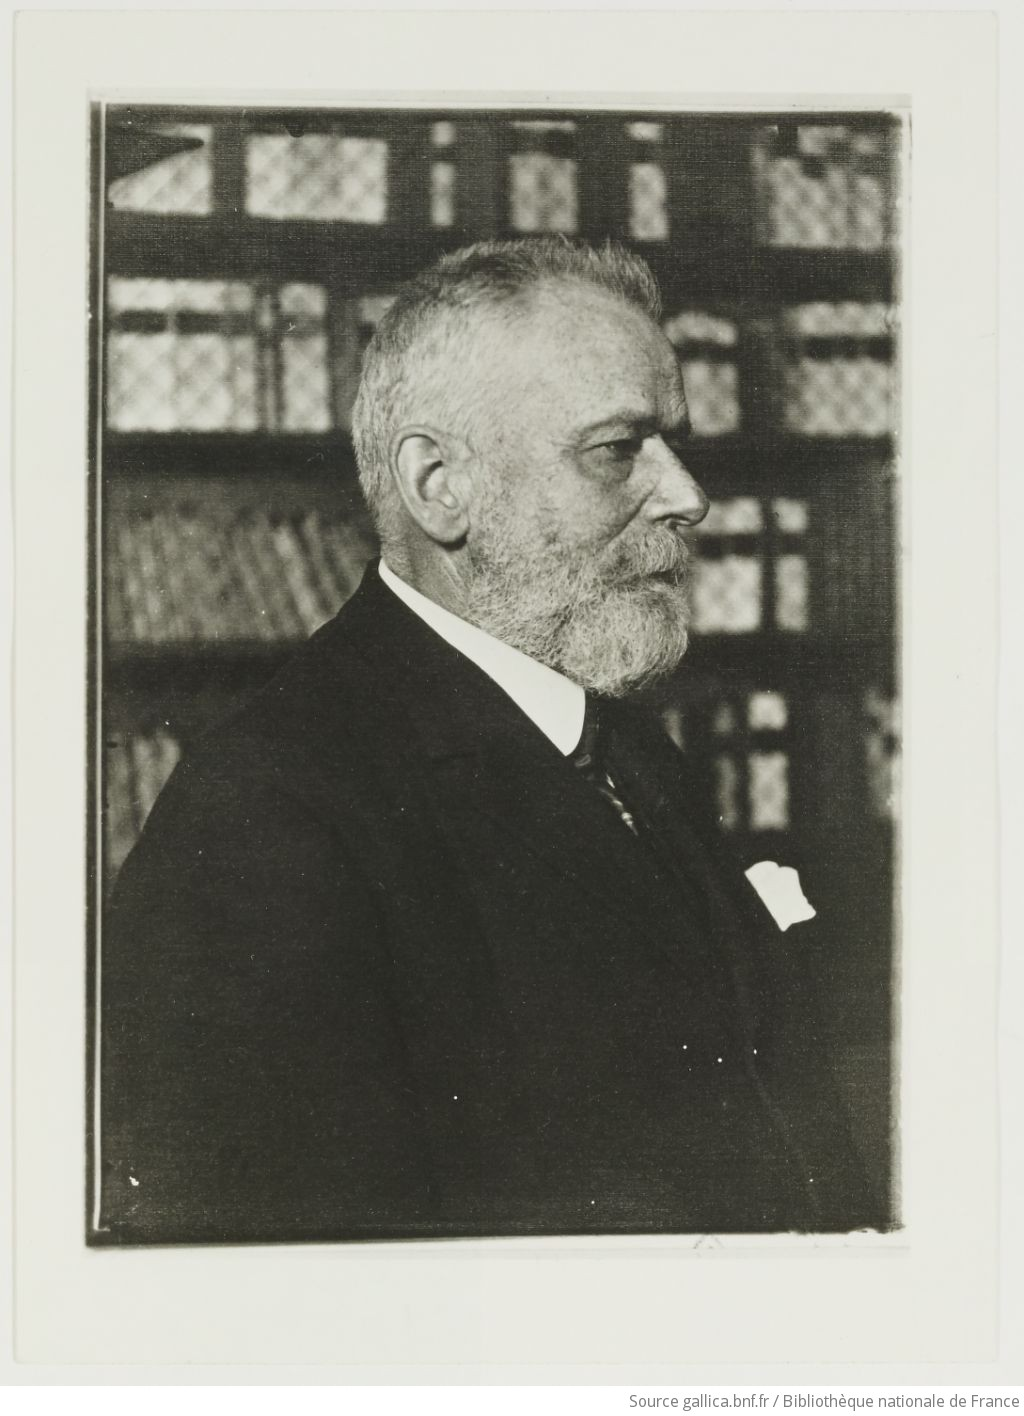
\includegraphics[width=10cm]{Images/rondel_portrait.jpeg}
    \caption{Portrait d'Auguste Rondel, (\enquote{Collection théâtrale Auguste Rondel. 1 - A Marseille et au Palais-Royal}, BnF ASP, 8-RT-3607(1)).}
    \label{fig:portrait-rondel}
\end{figure}

\begin{figure}[htbp]
    \centering
    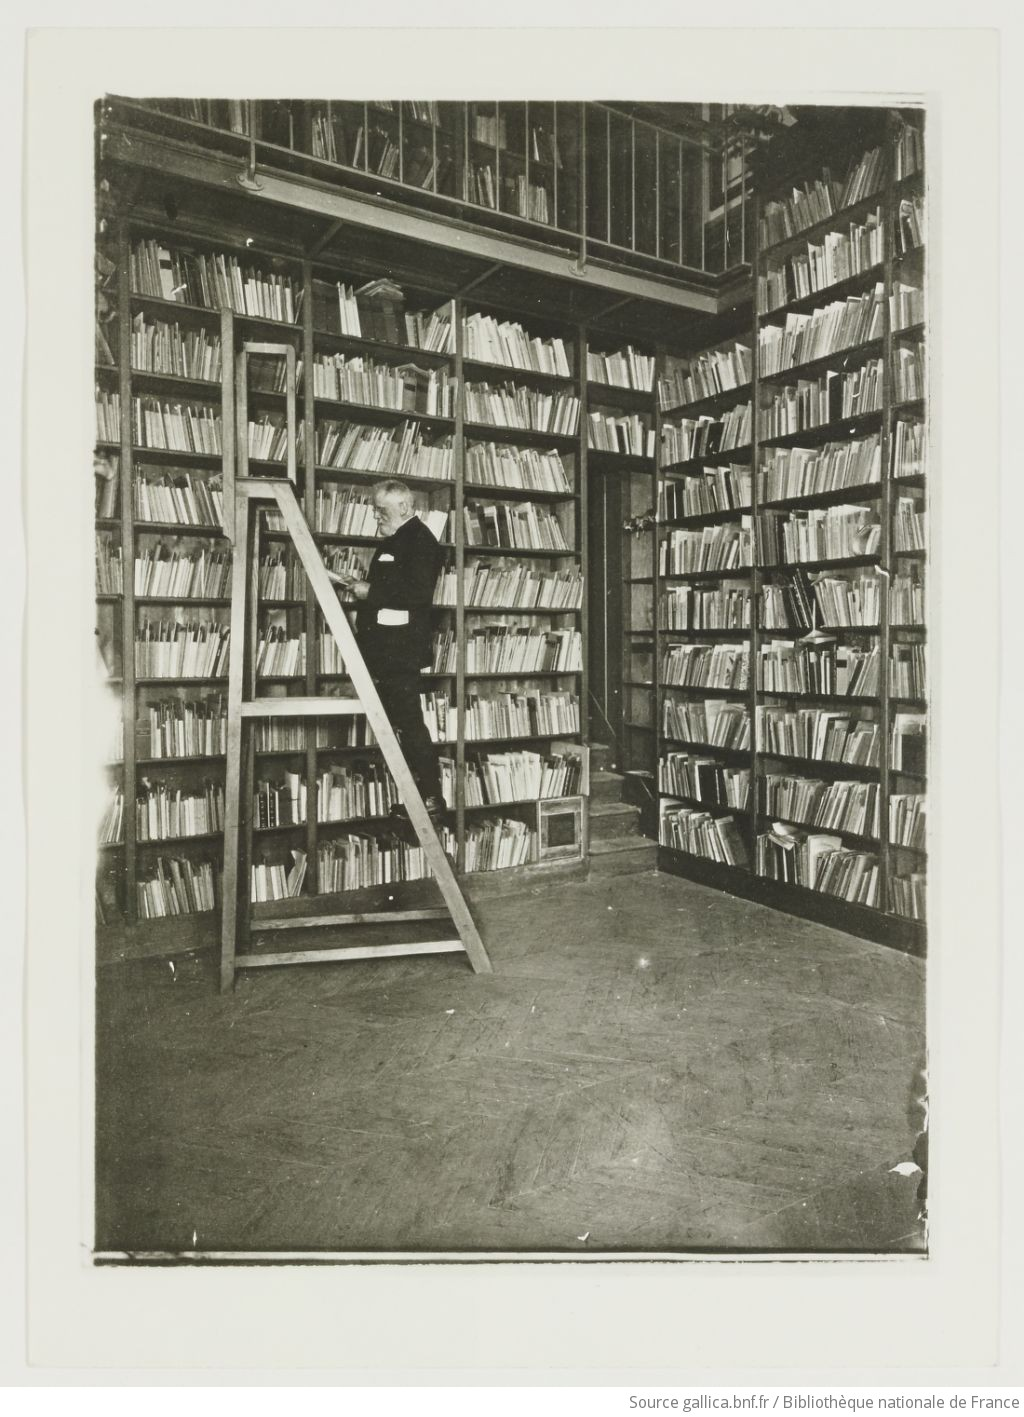
\includegraphics[width=10cm]{Images/RondelBibli2.JPEG}
    \caption{Auguste Rondel dans la salle des auteurs dramatiques du XX\textsuperscript{e} Siècle, (Comédie-française, Palais Royal, 1925), (\enquote{Revue d'histoire du théâtre}, 1958/IV, BnF ASP, 8-RT-3607(13)). }
    \label{fig:rondel-salle-auteurs}
\end{figure}


\section{Composition de la collection}

La collection Rondel regroupe des ouvrages de natures multiples, son fondateur étant \enquote{guidé par une vision encyclopédique et humaniste}\footcite[p. 265]{christout_2005}. Elle réunit de façon à la fois thématique et historique des manuscrits d'auteur, de la correspondance, des relevés de mise en scène, des notes de régie, des éditions rares, ou encore des affiches, des programmes ou des périodiques. Elle est également composée de documents iconographiques, tels que des estampes, des dessins ou des photographies. Rondel rejetait tout a priori, et s'intéressait, au-delà de tout clivage idéologique ou disciplinaire, à tous les genres. 
Son inventaire méthodique nous renseigne plus précisément sur la composition de la collection, dont voici les différentes sections : 


\vspace{1.5cm}

% Tableau en deux colonnes pour décrire la composition de la collection Auguste Rondel
\begin{tabular}{c|c}
\hline
  cote & section\\
\hline
  Ra & Fêtes\\
\hline
  Rae & Estampes : fêtes, spectacles de cour\\
\hline
  Re & Théâtre étranger\\
\hline
 Rf & Théâtre français\\
\hline
 Rj & Périodiques, mémoires, histoires littéraires\\
\hline 
 Rk & Cinéma\\
\hline 
 Ro & Musique\\
\hline 
 Rt & Histoire du théâtre\\
\hline
\end{tabular}

\vspace{1.5cm}


Dans la collection Rondel se trouve une forme particulière de document, créée par Rondel lui-même, qui consiste en un assemblage de coupures de presse sous forme de recueil, consacré à un sujet, une œuvre ou une période. Cette habitude qu'avait Auguste Rondel visait à simplifier la recherche future, en réunissant les sources sur un sujet.\footcite[p. 20]{themis_acrivopoulos_2013}. 

\begin{figure}[htbp]
    \centering
    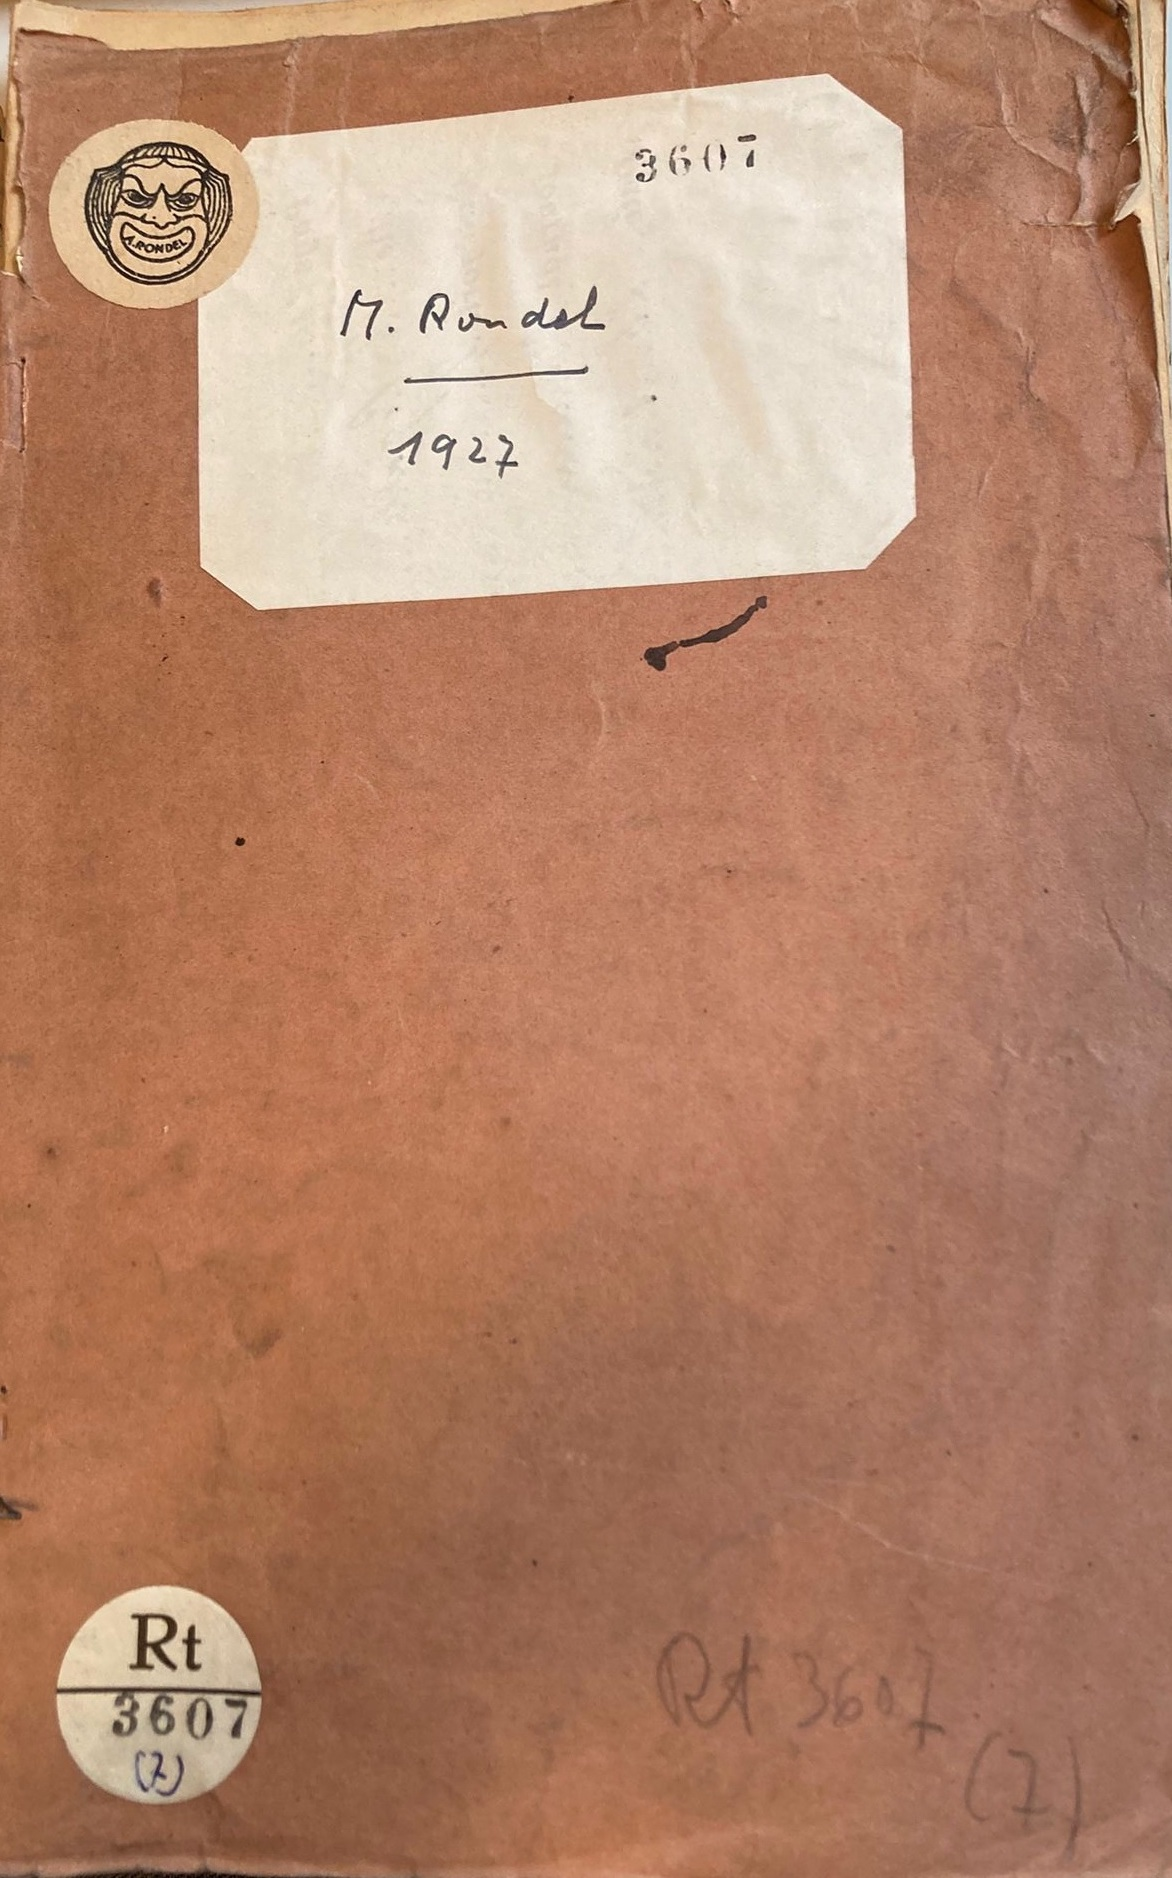
\includegraphics[width=10cm]{Images/RondelRecueilPresse.jpeg}
    \caption{Exemple de dossier de presse issu de la collection Rondel (\enquote{M. Rondel, 1927}, BnF ASP, Rt 3607(7)).}
    \label{fig:dossier-presse-rondel}
\end{figure}

\begin{figure}[htbp]
    \centering
    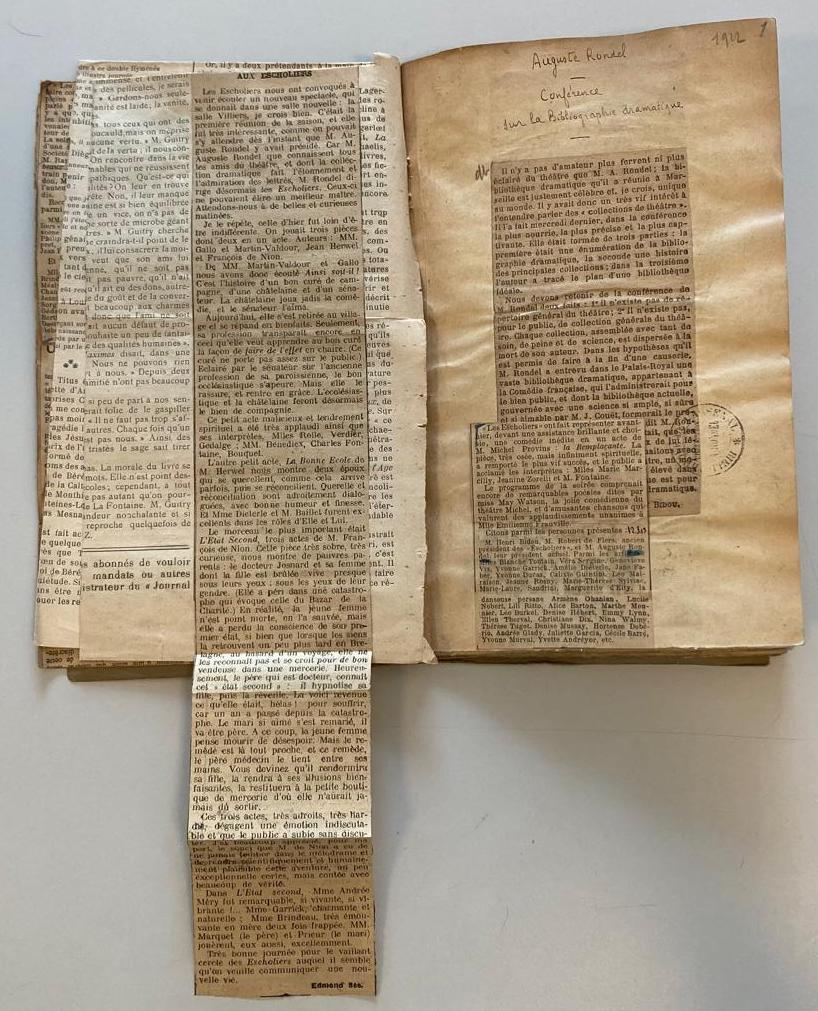
\includegraphics[width=7cm]{Images/RondelRecueilPresse2.jpeg}
    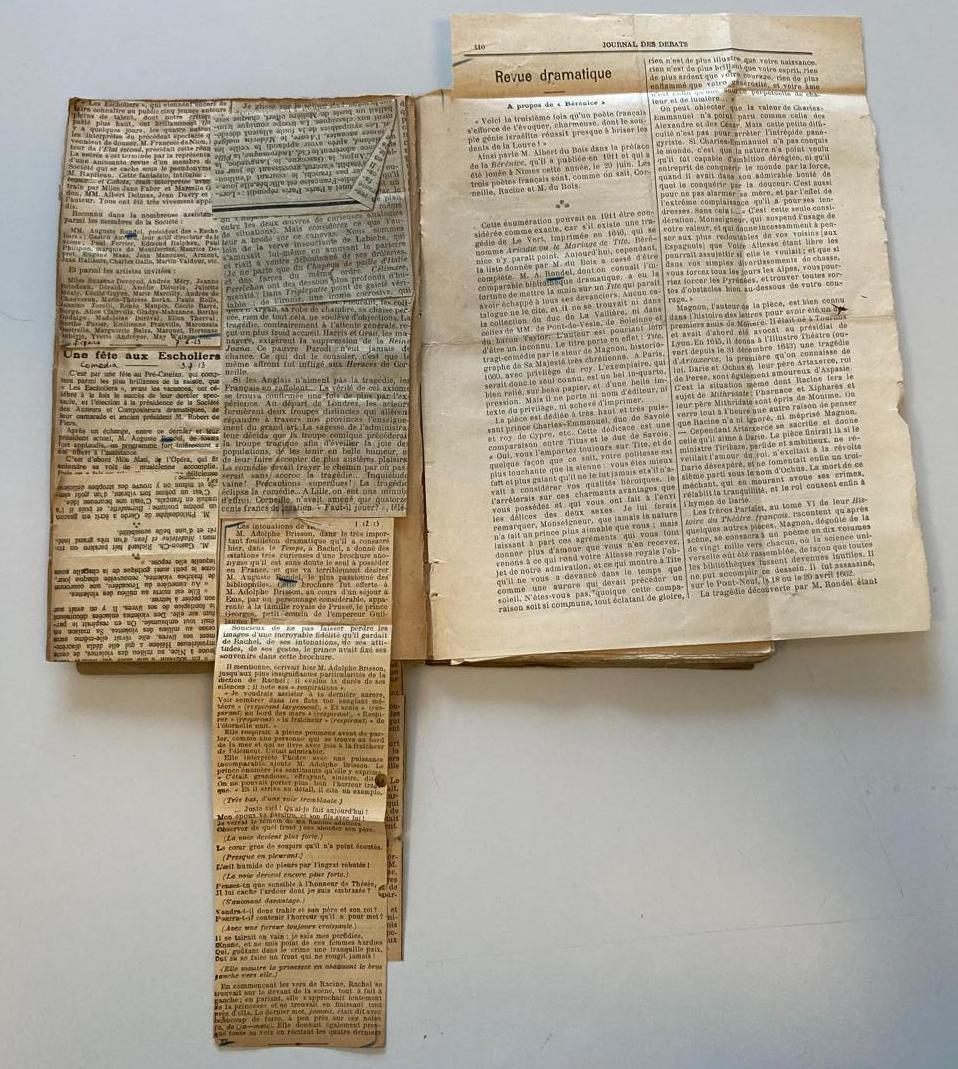
\includegraphics[width=8cm]{Images/RondelRecueilPresse3.jpeg}
    \caption{Coupures de presse, (\enquote{M. Rondel, 1912-1915}, BnF ASP, 8-RT-3607(3)).}
    \label{fig:coupures-presse-rondel}
\end{figure} 


\newpage


Ainsi, la collection constituée par Rondel lui-même compte trois cent mille volumes en 1918, et occupe à cette époque les deux étages de son hôtel particulier sur la place Saint-Ferréol à Marseille. Il consacre l'essentiel de sa fortune à sa collection, soit 7 millions-or en 1914, et lorsqu'il perd ses deux neveux à la guerre, il n'a plus d'héritier direct. Cela expliquerait peut-être en partie pourquoi il a demandé à l'État d'accepter la donation de sa collection et de la mettre à disposition du public à Paris, à la Comédie-Française, donation officialisée en 1920. Cela peut également s'expliquer par le fait qu'il redoutait que sa collection soit dispersée, comme l'ont été certaines bibliothèques théâtrales antérieures\footcite[Parmi ces collections dispersées, on peut citer celle de Charles Nodier en 1830 et 1844, celle de René-Charles Guibert de Pixerécourt en 1839, ou celle en 1864 de Charles-Simon Favart, créateur de la comédie musicale][p. 236]{thomas_2005}. Des crédits d'installation sont votés par la chambre en 1921, et l'inauguration a lieu en 1922. Dans ces nouveaux lieux, Rondel s'occupe de l'administration de sa collection, qu'il continue à enrichir, avec l'aide de Madeleine Horn-Monval. Née en 1886 et morte en 1972, Madeleine Horn-Monval est une bibliothécaire et historienne française, connue pour avoir été la collaboratrice d'Auguste Rondel et pour avoir administré sa collection\footcite[p. 185-188]{Antonutti_2020}. Après avoir travaillé dans l'enseignement, elle quitte ses fonctions pour assister Auguste Rondel dès 1920, et poursuit cette activité après la mort de Rondel, jusqu'en 1951\footcite[p. 43]{themis_acrivopoulos_2013}. Cependant, en septembre 1925, le ministre de l'instruction publique Anatole de Monzie ordonne à Rondel de quitter immédiatement le Palais-Royal sous prétexte de vouloir y loger à la place l'Institut international de coopération intellectuelle\footcite[p. 239-244]{giteau_2005}. Ce déménagement est d'ailleurs largement commenté par la presse de l'époque, comme en témoigne un dossier constitué par Rondel et consacré à ce  sujet\footnote{\enquote{Collection théâtrale Auguste Rondel. 2 - Transfert à l'Arsenal}, BnF ASP, Rt 3607(2).}.  

\begin{figure}[htbp]
    \centering
    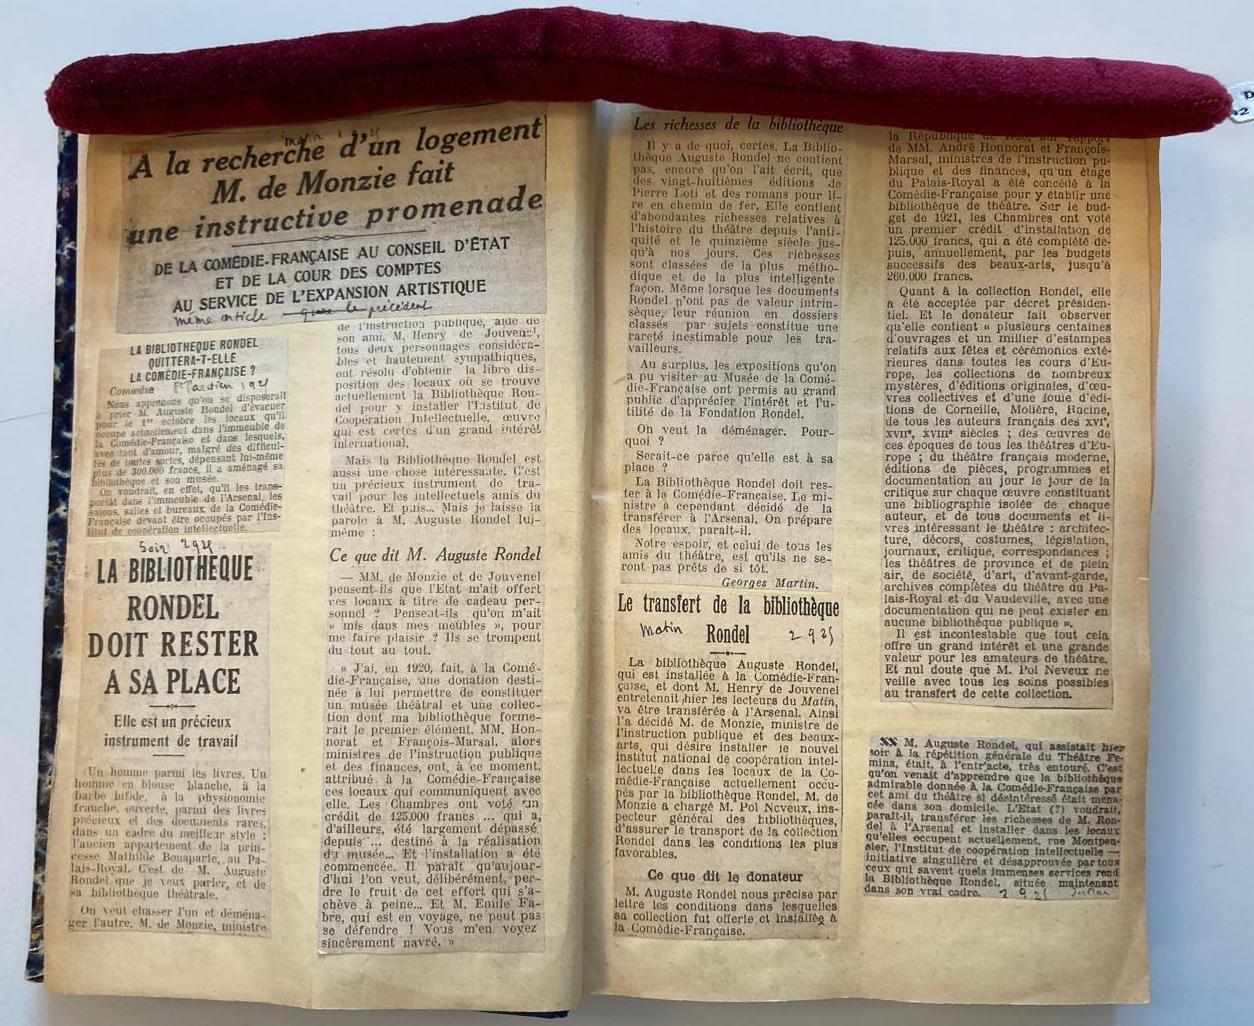
\includegraphics[width=15cm]{Images/coupures_presse_transfert_Arsenal.jpeg}
    \caption{Coupures de presse documentant et protestant contre le transfert à l'Arsenal de la bibliothèque Rondel, (BnF ASP, 8-RT-3607(2)).}
    \label{fig:transfert-arsenal}
\end{figure}


\section{Les archives d'Auguste Rondel, corpus utilisé dans le cadre de mon stage}

Le corpus documentaire utilisé dans mon stage est tiré des \enquote{Archives Rondel}, archives issues de l'activité d'Auguste Rondel et de Madeleine Horn-Monval. 
Les \enquote{Archives Rondel} sont constituées de la correspondance entretenue par Rondel, mais aussi des factures de près de 450 librairies auprès desquelles il a acheté des documents pour enrichir sa  collection entre 1900 et sa mort en 1934\footcite[p. 17-20]{bonicel_2006}. Ces factures proviennent surtout de France, Italie, Allemagne, Autriche, Pays-Bas, Belgique, Angleterre et Suisse. La mission principale de mon stage porte exclusivement sur ces factures, qui occupent une vingtaine de boîtes Cauchard de format quarto, dont l'épaisseur est de 8cm et occupant 1,60 mètres linéaires. 


\begin{figure}[htbp]
    \centering
    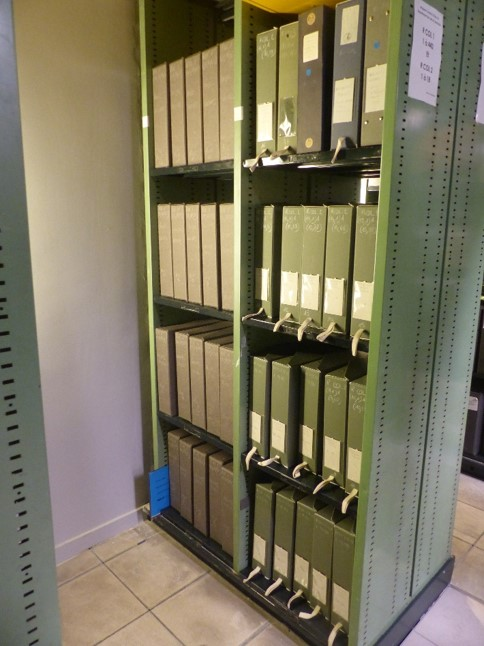
\includegraphics[width=10cm]{Images/boites_factures.jpeg}
    \caption{Factures Rondel, contenues dans les boîtes grises (étagère de gauche).}
    \label{fig:boites-factures}
\end{figure}


Nous nous sommes plus précisément concentrés sur un échantillon représentatif de ce corpus, composé de trois boîtes de factures sélectionnées par mon encadrante scientifique Hélène Keller. Les factures Rondel sont dans le catalogue BnF archives et manuscrits sous la cote RCOL, et chaque dossier est, en général, consacré à un libraire. Certains dossiers de factures contiennent également des extraits de correspondance entre le libraire et Rondel, qui parfois se confondent avec les factures, ou permettent de mieux les comprendre. 

Le type de papier utilisé dans les factures varie beaucoup selon le libraire et l'ampleur du corpus nous empêche d'en distinguer un en particulier. L'échantillon nous permet de dire que l'état de conservation des factures est très bon. Il y a parfois quelques plis et petites déchirures sur les bords de certaines factures, mais cela reste assez rare\footcite{constat_etat}. Les mandats de paiement, qui ont souvent été conservés et sont liés aux factures grâce à des trombones,  sont également en très bon état. Elles sont manuscrites pour la plupart, et le niveau de clarté, de lisibilité et de précision des informations est variable selon le libraire.  

Le nombre de titres écrits par facture varie entre un et une dizaine. Ils correspondent chacun à une ou plusieurs œuvres achetées par Rondel. Certaines factures, à l'image de celle que l'on peut voir ci-dessous, sont très complètes, et renseignent toutes les informations utiles pour identifier une œuvre. D'autres factures sont beaucoup moins détaillées, et ne contiennent que les informations les plus basiques, comme l'auteur, le titre et le prix. Il n'est parfois même pas possible d'identifier l'œuvre tellement le degré d'information est pauvre sur certaines factures. 

\begin{figure}[htbp]
    \centering
    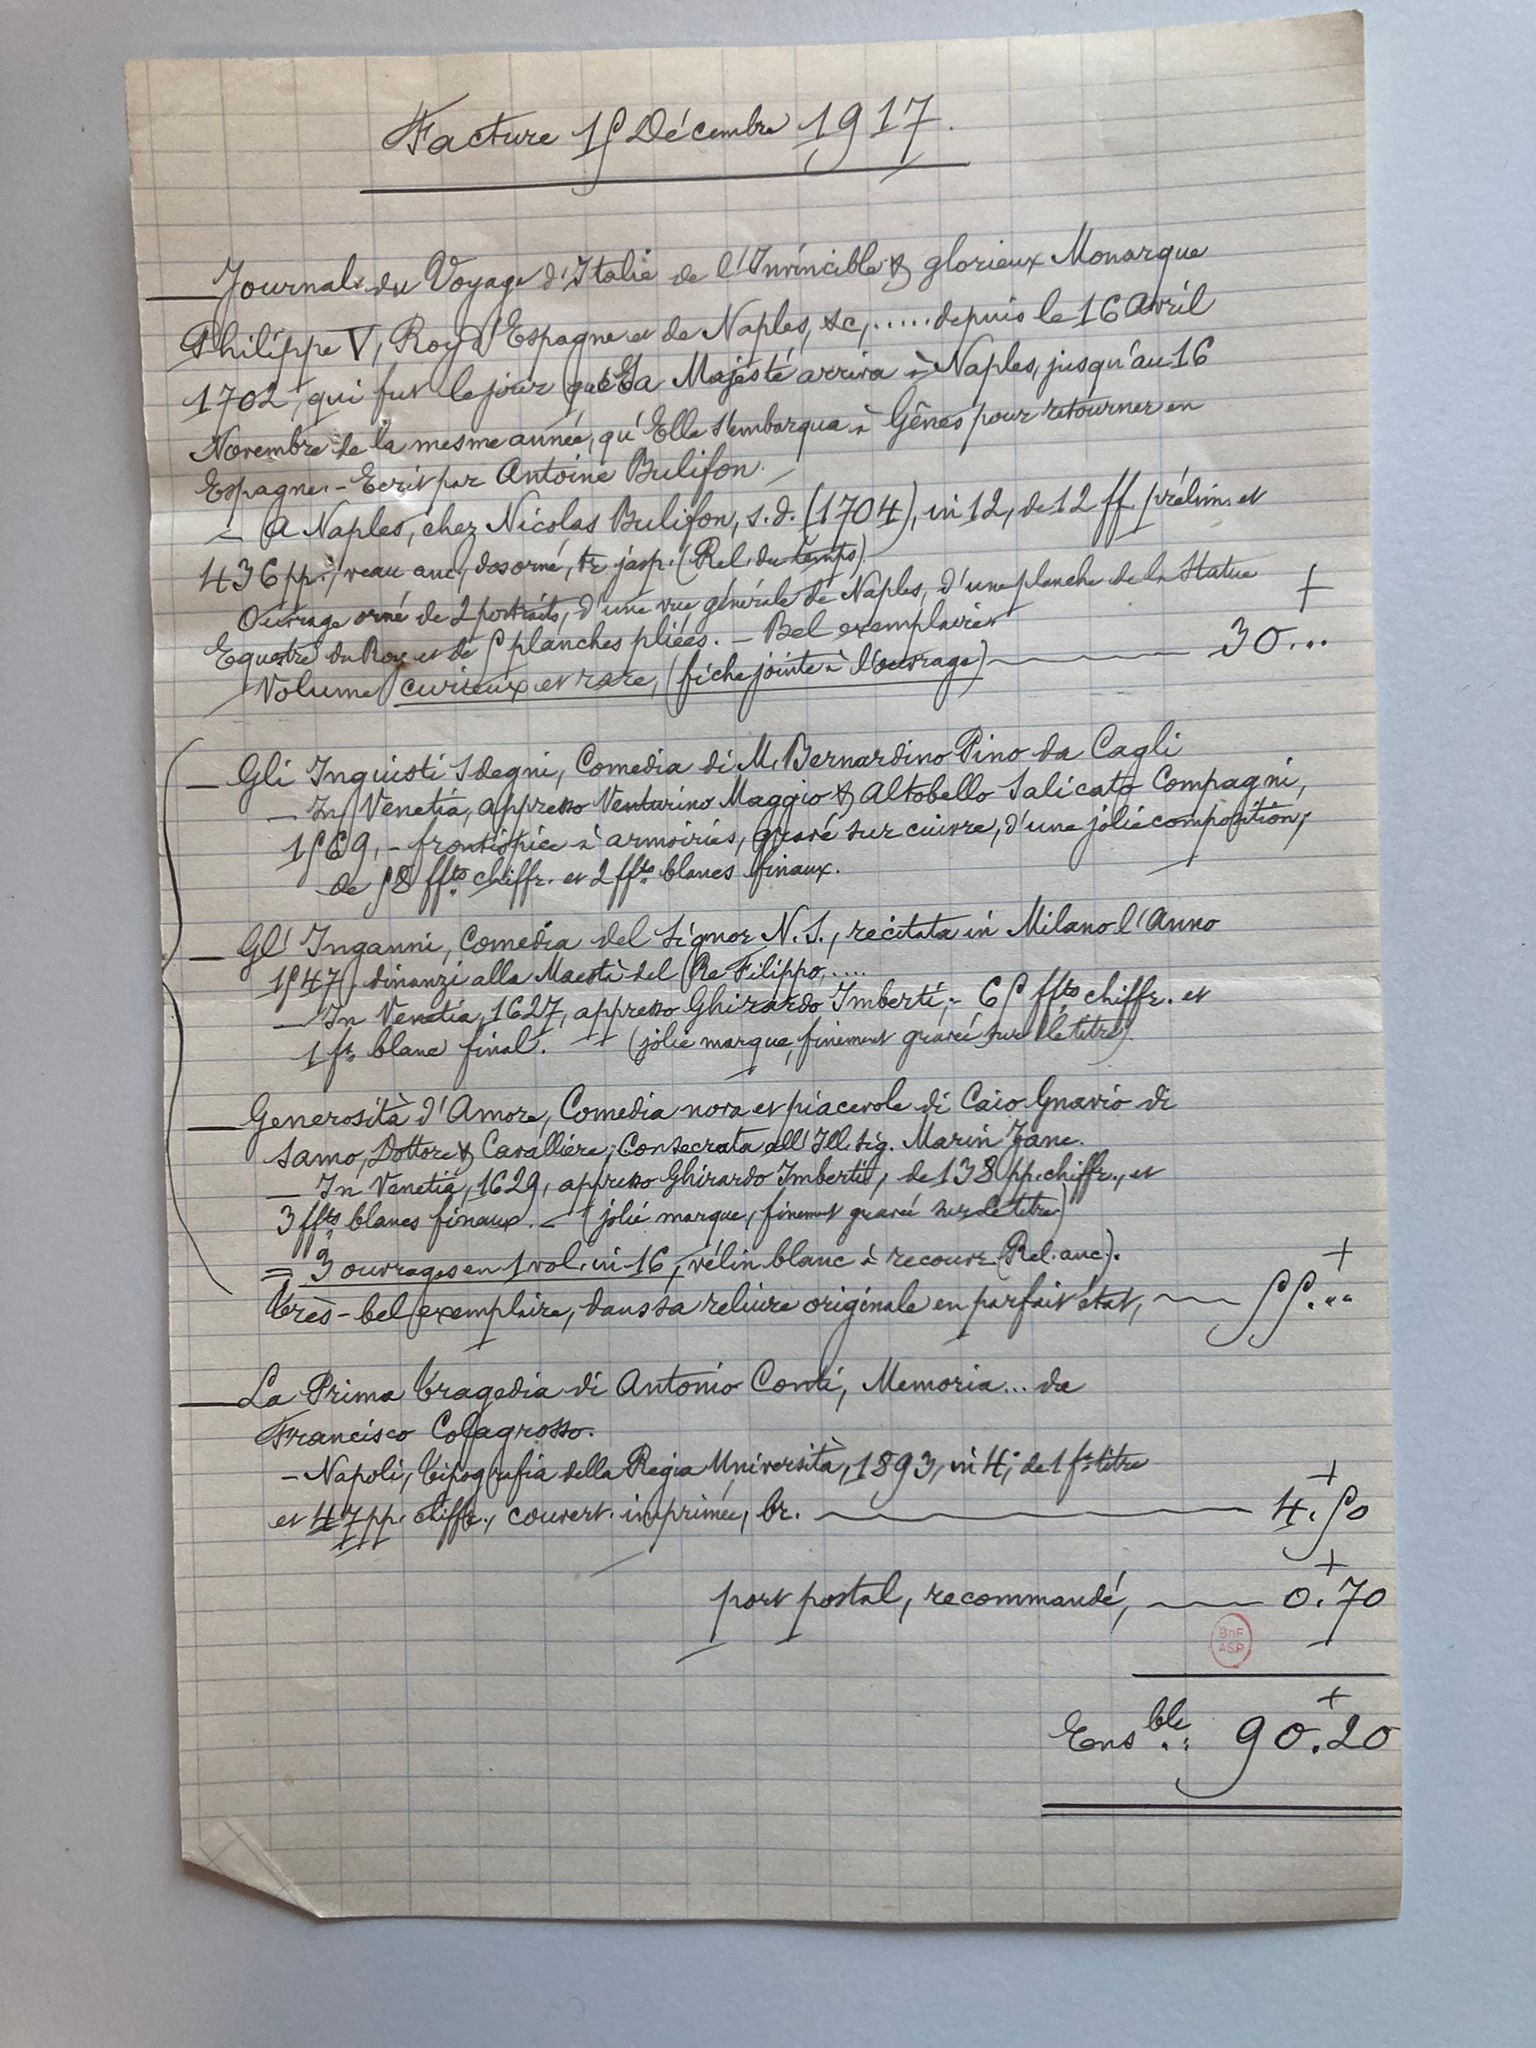
\includegraphics[width=10cm]{Images/Hermal_3.jpeg}
    \caption{Voici un exemple de facture dense et ordonnée : la facture Hermal du 15 décembre 1917 (BnF ASP, RCOL-1(220)).}
\end{figure}


Ainsi ont pu être introduits le parcours personnel d'Auguste Rondel et la constitution de sa collection, que notre projet de base de données a pour but d'étudier. Enfin, la présentation des archives d'Auguste Rondel, en particulier de ses factures, nous a permis de saisir l'ampleur et l'hétérogénéité du corpus à exploiter en vue de la modélisation de cette base.
\chapter{Etat de l'art : projets similaires}

Il convient de rappeler qu'un projet de base de données au sein de la BnF s'inscrit dans la continuité de travaux similaires réalisés auparavant. De même, l'utilisation d'\emph{Heurist} n'est pas inédite dans le domaine des sciences humaines et sociales, notamment à la BnF. 


\section{Les bases de données à la BnF}

Une base de données est un ensemble structuré de fichiers regroupant des informations ayant certains caractères en commun. Cet ensemble représente un système d'informations sélectionnées de façon à pouvoir être consultées par des utilisateurs ou des programmes\footcite{BDD_def}. Du fait des activités et de l'envergure de la BnF, la notion de base de données est très large dans le contexte de cette institution, et englobe toutes les données structurées, y compris les ressources les plus communément utilisées, telles que le catalogue général\index{Catalogue général de la BnF} ou Gallica\index{Gallica}.  
Ainsi, la base de données dont mon stage fait l'objet s'inscrit plutôt dans le contexte de la structuration de données en lien avec un projet de recherche. En effet, plusieurs programmes de recherche de la BnF ont abouti à la création de bases de données, qui donnent accès à des ressources spécialisées. C'est le cas de Mandragore, base de données scientifique dédiée à l’identification et à l'indexation de décors de manuscrits du département des Manuscrits et de la Bibliothèque de l’Arsenal. La base est mise en place en 1989 par le centre de recherche sur le manuscrit enluminé (CRME), qui est le fruit d'une collaboration entre le département des Manuscrits de la BnF et le CNRS. 
Parmi les bases de données venant de programmes de recherche réalisés à la BnF, certaines couvrent des thématiques assez proches de celles du projet Heurist sur les factures Rondel. Elles ont pu servir d'inspiration pour ce projet, qui s'inscrit dans leur continuité. La base \enquote{reliures}, par exemple, recense les reliures françaises à décor du XVI\textsuperscript{e} siècle au début du XIX\textsuperscript{e} siècle conservées à la réserve des livres rares de la BnF. Cette base a été utile à ma réflexion, car elle traite également du livre ancien dans sa matérialité et dans sa circulation, et s'intéresse aussi aux personnes exerçant des métiers liés au livre ancien. Dans la même veine, la base BP16 (\enquote{Bibliographie des éditions parisiennes du 16ème siècle}) recense, à partir des travaux de Philippe Renouard, toute la production imprimée à Paris au XVI\textsuperscript{e} siècle. Cette base a aussi été une source d'inspiration : je me suis inspiré de son exemple pour accorder une place centrale, dans ma base, aux exemplaires plus qu'aux oeuvres elles-mêmes. 
De plus, la base BP16 accorde une certaine attention aux libraires-éditeurs parisiens du XVI\textsuperscript{e} siècle, et l'un des objectifs de l'exploitation des factures Rondel est de faire une cartographie des libraires, notamment parisiens, fournisseurs de Rondel, ce qui place les deux projets dans la même continuité historique, et dans la continuité des pratiques professionnelles de l'institution. 

\section{Présentation et fonctionnement d'\emph{Heurist}}

\subsection{Histoire et présentation}


\emph{Heurist}\index{Heurist}, logiciel utilisé pour réaliser ce projet, est un système de gestion de base de données (SGBD) créé en 2005 par Ian Johnson, professeur à l'université de Sydney. \emph{Heurist} permet l'élaboration de bases de données relationnelles MySQL richement structurées\footcite{huma-num_heurist_2026}. Une base de données relationnelles (BDDR) est un type de base de données, qui se distingue par sa capacité à mettre en relation différentes données au sein de cette dernière.\footcite{marina_hervieu_2025}. Théorisé par un article intitulé \enquote{A Relational Model of Data for Large Shared Data Banks} et écrit par Edgar Codd en 1970, le modèle relationnel entend structurer les données sous forme de domaines (ensemble de valeurs) et de relations (tables). Ce modèle ne s'est pas imposé de manière universelle, mais a fortement influé sur les outils et pratiques de la base de données, du fait de ses nombreux atouts. En effet, la BDDR offre une représentation simple des données, n'étant constituée que de domaines et de relations, qui reste rigoureuse mathématiquement, puisqu'elle s'appuie sur la théorie des ensembles et des relations. Ce modèle est aussi révolutionnaire par sa capacité à décrire et à manipuler facilement les données, grâce à un langage unique qui s'est progressivement imposé\footcite[p. 45-47]{Hainaut_2015}. Il s'agit du SQL (\emph{Structured Query Language})\footcite[p. 191]{Hainaut_2015}, utilisé dès la fin des années 1970 et permettant de déclarer, de manipuler et d'interroger les données, mais aussi de contrôler leur accès\footcite[p. 166]{Soutou_2022}. 
Ces bases de données s'organisent sous la forme d'un ou plusieurs tableaux, appelés \enquote{tables}, contenant un ensemble de lignes. Une ligne est une suite de valeurs, et regroupe des informations concernant un objet. L'ensemble des valeurs de même type constituent une colonne. Les tables peuvent être liées entre elles par des colonnes particulières, appelées \enquote{clés étrangères}, dont le rôle est de référencer une table dans une autre\footcite[p. 44-54]{Hainaut_2015}. 


\emph{Heurist}\index{Heurist} est utilisé dans notre projet car il s'agit d'un logiciel particulièrement adapté aux projets de recherche en sciences humaines et sociales, et cela à plusieurs titres. En effet, ce logiciel a pour but de permettre aux chercheuses et aux chercheurs en sciences sociales de gérer leurs données acquises sur le terrain. L'enjeu est de leur redonner le contrôle sur leurs données, au lieu de le déléguer aux personnes en charge du développement informatique. Cela est permis par sa relative facilité d'utilisation : \emph{Heurist} est accessible par simple navigateur web et ne requiert aucune installation. De plus, il ne demande pas de compétences en programmation, c'est pourquoi il est accessible à un public relativement  large\footcite{huma-num_heurist_2026}. Ce logiciel est également apprécié du fait de son caractère \emph{Open source}, et de sa compatibilité avec les objectifs de la science ouverte. En effet, ses données peuvent être exportées dans des formats ouverts, comme le CSV, et sont accessibles sur le web et interopérables, notamment par la possibilité de publier un site web à partir d'une base de données\footcite{paillusson_introduction_2022}. 
\emph{Heurist} a été pensé pour résoudre des problématiques de recherche en SHS, c'est pourquoi il intègre des fonctionnalités en phase avec ces questions, telles que des visualisations temporelles ou spatiales\footcite{paillusson_introduction_2022}. 
Enfin, la considération suivante peut paraître secondaire, mais les logiciels spécifiques liés aux bases de données sont souvent appréciés par les chercheurs, car leurs formulaires de saisie sont plus \enquote{avenants}\footcite[Voir \enquote{Tableur ou gestionnaire de bases de données ?}]{Lemercier_Zalc_2008}. Ce détail a son importance, et fait partie des raisons pour lesquelles Heurist semble plus approprié qu'une base de données brute pour la recherche en SHS. 

\subsection{Les \emph{Records} et \emph{Record types}}

Les éléments au centre d'une base \emph{Heurist}\index{Heurist} sont les \emph{Records} et les \emph{Record types}. Le terme de \emph{Record type}, littéralement \enquote{type d'enregistrement}, est l'équivalent dans Heurist des tables d'une base de données, à savoir un ensemble d'objets de même nature. Ces Record types contiennent des \enquote{champs} (fields), c'est-à-dire des composantes qui fournissent leur structure, et correspondent aux colonnes d'une base de données. Les Records types et leurs champs sont d'ailleurs créés par la fonction \enquote{Design} du logiciel. Les champs sont aussi appelés \enquote{attributs} dans le contexte d'une base de données. Ces champs sont complétés par des \emph{Records}, qui sont des instances de ces tables, constitués de données qui remplissent les différents champs. Lorsqu'un champ est obligatoire (\enquote{mandatory}), l'enregistrement ne peut pas exister si ce champ là n'est pas rempli par des données. Le champ peut aussi être recommandé (\enquote{recommended}), facultatif (\enquote{optional}) ou caché (\enquote{hidden}). Dans le dernier cas, le champ n'apparaît pas lorsque l'on affiche les enregistrements de cette table. 

\subsection{Les types de données}
\label{types donnees}

Comme une base de données classique, \emph{Heurist}\index{Heurist} offre la possibilité de choisir le type de données que l'on veut utiliser pour chaque champ. Cependant, les types de données proposés par Heurist sont très spécifiques à ce logiciel, c'est pourquoi il convient de les détailler ici. Tout d'abord, \emph{Heurist}\index{Heurist} propose deux types de données textuelles : text (single-line), qui n'autorise qu'une seule ligne de texte, et sert à renseigner des noms ou des descriptions courtes, et memo text (multi-line), utile pour les paragraphes. Pour les nombres, le type de données \emph{Numeric} permet de renseigner des nombres positifs ou négatifs, entiers ou décimaux. En base de données relationnelles, les données numériques peuvent aussi être générées automatiquement dans une colonne dédiée, afin de donner à chaque enregistrement d'une table un identifiant unique. Il s'agit de générateurs de séquences de valeurs, appelés différemment selon le SGBD, mais souvent par le terme \emph{autoincrement}\footcite[p. 194]{Hainaut_2015}. \emph{Heurist}\index{Heurist} permet aussi de générer des identifiants numériques pour chaque enregistrement d'une table, en rendant un champ numérique obligatoire et en cochant la case \emph{Increment value by 1}. Il faut noter qu'un autre identifiant est généré automatiquement à chaque enregistrement dans \emph{Heurist}\index{Heurist}, peu importe son \emph{Record type} : l'\emph{Heurist identifier}, aussi appelé \emph{Heurist-ID}. Les \emph{Heurist-ID} servent surtout à être lus par le logiciel et à être reliés à des enregistrements déjà existants en cas d'imports de données en masse. La gestion des dates est très pratique dans \emph{Heurist}\index{Heurist}, grâce au type de données \enquote{Date/temporal}, qui permet d'avoir différentes échelles de précision sur les dates que l'on renseigne. En effet, on peut choisir si on entre une date exacte dans la base, au format YYYY-MM-DD, ou une date approximative, ce qui affichera dans la base le terme \enquote{circa} suivi de la date. Il est aussi possible d'indiquer une date avant ou après laquelle a eu lieu l'évènement qu'on souhaite dater, ce qui indiquera \enquote{before} ou \enquote{after} suivi de cette date. On peut aussi renseigner un intervalle de dates, et des degrés de certitude pour chaque date renseignée, à savoir \emph{Unknown} (inconnue), \emph{Attested} (attestée), \emph{Conjecture} (supposition) ou \emph{Measurement} (estimation). 
Les données de type \emph{Dropdown} sont l'une des spécificités d' \emph{Heurist}\index{Heurist}. Il s'agit d'un choix déroulant entre différents mots de vocabulaire, issus de listes que l'on définit dans une fonctionnalité spéciale du logiciel, appelée \emph{Vocabularies} (vocabulaires contrôlés). Les vocabulaires contrôlés permettent donc d'avoir des listes de mots, pré-conçues pour remplir certains champs, ce qui évite de tout devoir saisir à la main. Il existe également un type de données nommé \emph{File or remote URL} et permettant d'importer des fichiers ou une URL. 


\subsection{Les relations}

Certains types de données dans \emph{Heurist}\index{Heurist} servent à lier différents Record types entre eux, ce qui est l'intérêt d'une base de données relationnelle. Ces types de données sont le \emph{Record pointer} et le \emph{Relationship marker}. Les Record pointers sont l'équivalent dans \emph{Heurist}\index{Heurist} des clés étrangères dans une base de données classique : ils servent à lier une table à une autre. Lorsque l'on crée un champ de ce type, il faut d'abord choisir à quel \emph{Record type} on veut faire la liaison, et pour remplir ce champ, il faut sélectionner l'enregistrement auquel on veut lier celui qu'on est en train de créer. Les \emph{Relationship markers}, deuxième type de relation possible, consistent encore une fois à lier deux enregistrements entre eux, mais cette fois avec la possibilité de préciser quel type de relation existe entre ces enregistrements. Ce type de données permet également de décrire et de mettre des bornes chronologiques à ces relations. Tout comme les \emph{Dropdown}, les \emph{Relationship markers} font aussi appel à des vocabulaires contrôlés que l'utilisateur peut concevoir lui-même au préalable. 

En somme, \emph{Heurist} est un logiciel permettant de créer et de gérer des bases de données relationnelles, selon des types de données qui lui sont propres. 

\section{Projets \emph{Heurist} similaires à celui des factures Rondel}

Cette utilisation fréquente d'\emph{Heurist} dans des projets de recherche en SHS fait que le nôtre s'inscrit dans la continuité de projets précédents, traitant les mêmes thématiques. 

Le projet DEF-19 (Dictionnaire des éditeurs français du XIX\textsuperscript{e} siècle) a été financé par l'ANR entre septembre 2014 et septembre 2019, et a notamment consisté à la mise en place d'une base de données \emph{Heurist}\index{Heurist}. Celle-ci est composée de deux tables : une consacrée aux personnes (éditeurs) et une aux établissements (maisons d'édition). Ainsi, chaque établissement est lié aux personnes qui le composent. Cette base présente également les données sous forme cartographique, où l'utilisateur peut affiner sa recherche pour sélectionner ce qu'il souhaite voir sur la carte\footcite{noauthor_dictionnaire_nodate}. Cette base nous a également inspiré, car elle traite, une fois de plus, les mêmes thèmes que la nôtre. Nous nous sommes donc inspirés de sa structure, qui était assez claire, pour modéliser les liens entre les personnes et les établissements. 

\section{Projets \emph{Heurist} déjà réalisés à la BnF}


La conception d'une base \emph{Heurist} au sein du département des Arts du spectacle participe du déploiement du logiciel à la BnF. Au-delà des autres raisons évoquées précédemment, qui font d'\emph{Heurist} un logiciel adéquat pour les projets de recherche en sciences humaines, le logiciel convient parfaitement au contexte humain et professionnel d'une institution patrimoniale aussi vaste que la BnF. En effet, \emph{Heurist} peut rapidement être pris en main par différentes personnes, sans qu'elles aient nécessairement de connaissances techniques sur les bases de données. On peut donc aisément imaginer des membres d'un ou plusieurs services (ou département) utiliser la même base \emph{Heurist}, que ce soit pour l'implémenter ou pour chercher des informations dedans. \emph{Heurist} peut également être apprécié à la BnF pour sa capacité à s'imposer dans le temps. Son utilisation est très guidée, et les bases peuvent contenir une grande quantité de documentation. En effet, le logiciel prévoit, au sein de chaque élément de la base, (\emph{Record type}, \emph{fields}), des espaces de textes pouvant accueillir des indications sur l'utilisation qu'il faut en avoir. 
C'est pourquoi une base \emph{Heurist} pourrait perdurer et survivre par exemple à un renouvellement d'équipe. Le logiciel se prête donc très bien à l'exploitation d'un corpus aussi large que les factures Rondel, qui devra être réalisée sur une longue période et par plusieurs personnes. 
Ainsi, plusieurs bases \emph{Heurist}\index{Heurist} ont déjà été créées au sein de la BnF, avec différents niveaux d'aboutissement. 

\subsection{Collections de collectionneurs}

La base \emph{Heurist} \enquote{Collections de collectionneurs} est une composante du projet de recherche éponyme, mené par la bibliothèque de l'Arsenal et inscrit au plan quadriennal de la recherche pour la période 2020-2023\footcite{noauthor_plan_nodate}. 
Ce projet est assez proche, dans sa thématique, de celui entrepris pendant mon stage, et part du constat que les catalogues actuels de la BnF ne sont pas adaptés à l'analyse des anciennes collections bibliophiliques qu'elle conserve, alors qu'elles font l'objet de travaux par des chercheurs et des conservateurs. L'objectif est donc de créer un modèle de données spécifique pour permettre une meilleure description, visualisation et gestion de ces collections de bibliophiles. Le but est également de s'intégrer aux systèmes d'information de la BnF et d'assurer la pérennisation des données.

En effet, cette base \emph{Heurist}\index{Heurist} décrit avec précision les ouvrages issus de ces collections. Les informations sont requêtables grâce aux recherches filtrées permises par le logiciel, portant une attention particulière à la matérialité des livres (reliure, tranche, décors)\footcite{noauthor_collection_nodate}. 


\subsection{Base des trésors monétaires}

La base de données \enquote{Trouvailles monétaires} recense l'ensemble des dépôts monétaires découverts sur le territoire français et les données venant des archives du département des Monnaies, médailles et antiques de la BnF. Le département porte le programme de recherche éponyme depuis 1978, avec pour ambition d'étudier et de valoriser les découvertes numismatiques. La base s'est développée grâce au soutien de deux plans quadriennaux de la recherche entre 2016 et 2023, et se poursuit grâce à l'ajout de nouvelles données, notamment via le projet Archinumis (2024-2027), qui enrichit la base par l'étude d'archives numismatiques\footcite{noauthor_base_nodate}. Aujourd'hui, plus de 200 trésors et 230 000 monnaies sont publiés. 
Beaucoup de tables composent cette base, mais les principales sont les tables \enquote{Ensemble}, qui décrit les monnaies provenant de trésors, monnaies d'or isolées ou dépôts monétaires du territoire national, mais aussi les monnaies issues de fouilles, \enquote{monnaies} et \enquote{objets}. Ces tables piochent leurs informations dans des tables de listes fermées, ce qui évite les doublons. Dans la base, les ensembles sont notamment visibles sous la forme d'une frise chronologique. 

\subsection{Répertoire des mains musicales}

Le projet est mené par le département de la Musique de la BnF depuis 2020, et vise à faciliter l'identification des écritures musicales, utilisant des technologies de data mining et de reconnaissance de formes. La base de données, qui est le premier volet, s'organise autour de trois entités : les scripteurs, les manuscrits et les signes musicaux et compte actuellement 152 scripteurs, 359 manuscrits et 3454 signes musicaux. Le deuxième volet du projet consiste à utiliser l'intelligence artificielle pour développer un outil informatique capable de reconnaître les scripteurs de manière automatique\footcite{noauthor_repertoire_nodate}. 
 

\section{Conclusion de la première partie}

En somme, ce besoin de modélisation d'une base de données dans le cadre de l'exploitation des factures Rondel s'explique par l'importance qu'a la collection Rondel dans l'histoire du département, étant à la fois l'origine et le cœur de ses collections. De plus, au vu de leur quantité et de leur diversité, les factures de librairie qui composent les \enquote{Archives Rondel} pourraient nous fournir de nombreuses informations sur la collection, et seraient donc un corpus particulièrement utile à la recherche sur le sujet. Le thème des provenances suscite actuellement un grand intêret dans les établissements patrimoniaux. La forme d'une base de données, privilégiée dans la réalisation de ce travail, a déjà été utilisée à plusieurs reprises, par différents départements de la BnF. Quelques-unes ont déjà été créées avec \emph{Heurist}\index{Heurist}, c'est pourquoi notre projet s'inscrit dans la continuité du déploiement de ce logiciel \emph{Open source} à la BnF.

%etc
	
	\part{Réalisation technique : une base de données \emph{Heurist} sur les factures Rondel}

Cette deuxième partie entend présenter toutes les étapes du travail technique réalisé afin d'exploiter les factures Rondel de la manière la plus pertinente possible. Il s'agira donc de retracer toute l'analyse des documents, dans le but d'en extraire les informations utiles et de modéliser une base de données, puis de la concevoir à l'aide d'\emph{Heurist}\index{Heurist}. Nous nous demanderons enfin à quels besoins cette base de données peut répondre, en matière de datavisualisation et de recherche. 

\chapter{Travail préparatoire et complémentaire à la modélisation de la base de données}

La conception de cette base de données n'a pas pu être possible sans un travail préalable de réflexion et de modélisation, totalement extérieurs à l'utilisation d'\emph{Heurist}. 

\section{Analyse des documents en vue de leur exploitation}

Pour pouvoir tirer un maximum d'informations des factures Rondel, et surtout pour en extraire les données pertinentes à entrer dans la base, il convient d'abord d'analyser la façon dont elles sont structurées. C'est pourquoi a d'abord effectué un travail de consultation et de lecture proche des sources. La lecture attentive, ou \emph{close reading}, est une méthode issue de la critique littéraire consistant en une analyse minutieuse des sources. 
Cependant, le but ici n'est pas de faire une étude exhaustive de la composition des factures, car vu le volume du corpus, ce travail serait trop long à réaliser. Il s'agit simplement, à partir de l'échantillon sélectionné, de repérer quelles sont les informations importantes et récurrentes dans ces factures, afin de réaliser un modèle qui, bien que précis, soit suffisamment général pour pouvoir s'adapter aux différents cas de figure susceptibles d'apparaître dans l'ensemble de ces documents. Plus qu'une obligation, l'absence d'exhaustivité dans l'analyse des documents, puis dans la modélisation des données est même un parti pris, car prendre en compte tous les cas de figure serait impossible, et n'aurait aucun intérêt. Il a donc été établi que les informations qui apparaissent le plus souvent, ainsi que celles permettant d'identifier les factures, les personnes, et surtout les œuvres devront faire partie de la base.

Cette première analyse nous a permis de regrouper certaines catégories d'informations cohérentes entre elles. Cela nous a également fait réfléchir à des premières ébauches de tables de notre future base de données.

Nous nous sommes d'abord concentrés sur les informations qui apparaissent systématiquement concernant les librairies, à savoir leurs noms, adresses et villes. Nous avons également constaté que leur spécialité apparaissait parfois dans les factures, mais que ce n'était pas systématique. 
Nous avons aussi remarqué certaines informations, souvent discrètes, qui concernent des personnes dans les factures. Il s'agit parfois des signataires des documents, ou simplement des personnes mentionnées comme étant propriétaires ou employés de la librairie. Les informations sur les personnes sont particulièrement présentes dans des extraits de correspondances qui se trouvent dans les dossiers à côté des factures. A aussi été envisagée la nécessité de regrouper les informations qui concernent les factures elles-mêmes, telles que leur date, le nombre d'oeuvres achetés dans chaque facture ou les éventuels commentaires parfois inscrits en bas des factures. Dans ce cadre, une attention particulière a été prêtée au montant total, à la date du paiement et à la présence ou non d'un mandat de paiement. Nous avons donc tiré de ces observations la nécessité d'avoir dans notre base une table dédiée aux factures, pour pouvoir retrouver précisément chaque facture, afin de retracer l'origine des informations qui en sont issues. Sont ensuite venues les réflexions sur les données au centre de ce travail sur les factures, à savoir les informations sur les documents achetées par Rondel, qui se trouvent dans les lignes de ces factures. Comme nous l'avons évoqué précédemment, les informations concernant les documents peuvent être multiples (auteur, date, lieu, format, numéro dans le catalogue du libraire) : il a donc fallu les relever de manière exhaustive, pour couvrir tous les cas possibles.

Cette analyse de notre échantillon de factures nous a permis de regrouper les informations les plus importantes, afin de dégager des hypothèses de futures tables de la base de données. Ce travail s'est rapidement suivi de premières modélisations. 

\section{Modélisation et réflexion sur la structure de la base}


Une des étapes nécessaires à la conception d'une base de données est la modélisation, qui consiste à créer la représentation d'un système complexe afin de l'étudier, de le manipuler, de le comprendre. En informatique, modéliser revient donc à établir une logique formelle d'un domaine pour permettre à la machine de le manipuler ou de le calculer\footcite{bermes_2025}.  
Plus que nécessaire, la modélisation est un processus crucial dans la conception d'une base de données, car cela conditionne la structure de la base et influencera donc les performances à venir. Il en existe plusieurs formes, qui correspondent à différents niveaux de précision, et peuvent être réalisées de manière successive lors de la conception d'une base de données. Le premier type, souvent réalisé dans un premier temps, est le modèle conceptuel de données (MCD), qui est une représentation abstraite de la base de données, ayant pour but de modéliser les données qui seront stockées, sans décrire complétement le système. La modélisation conceptuelle se concentre sur les aspects sémantiques du modèle de données, sans aucune indication relative aux structures de stockage ou d'accès aux données\footcite[p. 13]{Soutou_2022}. Le modèle physique présente les données telles qu'elles seront stockées dans la base. Sans négliger le niveau conceptuel, nous avons choisi, dans la modélisation de notre base de données, de nous inspirer de l'étape intermédiaire : le modèle logique de données (MLD), aussi appelé \enquote{schéma relationnel de base de données}\footcite[p. 145]{Bergougnoux_2019}. Plus précis que le modèle conceptuel, ce niveau de modélisation représente les tables de la base de données, et caractérise les liens entre ces tables par la représentation de clés étrangères.



Le modèle de données conçu dans le cadre de notre projet a, dans un premier temps, été réalisé avec le logiciel \emph{Draw.io}\index{draw.io}, outil en ligne de modélisation de diagrammes, particulièrement adapté à la création d'architecture de bases de données, permettant de représenter leur structure\footcite{drawio}. 
Notre modèle est très spécifique : les types de données et les liens entre les tables qu'il décrit ne correspondent pas à ceux que l'on trouve dans des bases de données plus classiques, mais à ceux d'\emph{Heurist}, que nous avons présentés dans le chapitre précédent. Cependant, pour pouvoir représenter de manière précise les liens entre les tables, nous avons choisi de conserver une représentation communément utilisée dans les modèles de données, inspirée du formalisme de Barker, qui est un style graphique de modélisation des données. Les liens entre les tables sont donc représentés par une notation dite \enquote{Crow's foot} (en patte de corbeau), qui permet de modéliser la nature de ces liens par des flèches et des symboles\footcite[p. 7]{Hainaut_2015}. Cette étape peut paraître anecdotique, mais est essentielle car elle va permettre de définir les cardinalités, c'est-à-dire le nombre d'objets concernés par chaque lien\footcite[p. 32]{Soutou_2022}. 
Le modèle de données est visible dans l'annexe A\footnote{Voir \enquote{\nameref{modele donnees}}.}. 


Pour des besoins de clarification, mais également à des fins de communication a été réalisée une représentation simplifiée de ce modèle de données, inspirée des bases \emph{Heurist} précédemment réalisées à la BnF. Ce schéma reprend les différentes tables de la base, et représente par des flèches les liens qui les unissent. Ces flèches se concentrent davantage sur la circulation des données entre les tables que sur la nature des liens. 

\begin{figure}[htbp]
    \centering
    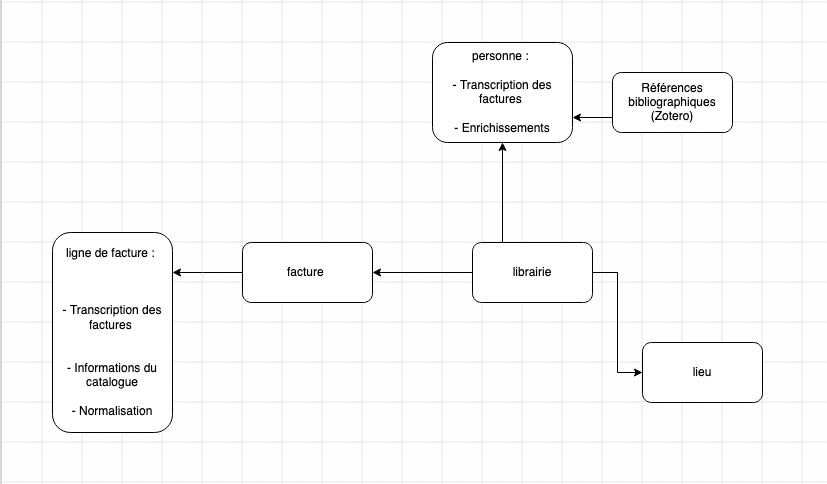
\includegraphics[width=10cm]{Images/modele simplifie.png}
    \caption{Représentation simplifiée du modèle de données.}
    \label{fig:modele-donnees-simplifie}
\end{figure}


Pour ne pas être perdus de vue, les objectifs de la base de données doivent être circonscrits dès le début du projet. Pour ce faire, nous avons utilisé dans ce travail préparatoire un autre outil, moins caractéristique de la modélisation de bases de données, mais plutôt utilisé dans le développement de produits : le \textit{Minimum Viable Product} (MVP). Le principe est de lister les fonctionnalités d'un produit, afin de les hiérarchiser selon un ordre de priorité de développement. Le but principal de cet outil correspondait parfaitement à notre besoin, à savoir d'avoir rapidement un produit fonctionnel pour pouvoir l'expérimenter et recueillir des retours d'utilisateurs\footcite[p. 60]{hervieu_2024}.

Un MVP a donc été réalisé au tout début de ce travail. Les fonctionnalités imaginées ont été partagées en plusieurs catégories. Les \textit{Must have} du projet sont ses éléments essentiels, dont la réalisation a un impact fort et demande un effort acceptable. Les \textit{Can be done} sont réalisables avec un effort minimal et un faible impact sur le projet final. Les fonctionnalités dites \enquote{\textit{Nice to have}} sont supplémentaires et non essentielles. Enfin, les fonctionnalités considérées comme \textit{Out of MVP} sont hors de portée, irréalisables ou constitueraient une grande perte de temps. Ces fonctionnalités ont été représentées par couleur et dans un tableau. Pour des raisons de lisibilité, le document issu de cette réflexion est, lui aussi, disponible dans l' annexe A. Celui-ci a été schématisé sur \emph{draw.io}\index{draw.io}, dans un tableau assorti d'une légende\footnote{Voir \enquote{\nameref{MVP}}}. 


Pour résumer cette réflexion, il a surtout été établi que la priorité absolue, dans la conception de cette base de données, était de reprendre toutes les données venant des factures. Les autres fonctionnalités imaginées n'étaient pas obligatoires, et pouvaient être réalisées dans l'immédiat si le travail n'était pas trop long à faire, ou plus tard. 

\section{Réception et utilisations de cette base de données}

Que ce soit en amont de sa création, tout au long de la modélisation ou de la conception de cette base de données, il convient de prendre en compte les besoins de ses potentiels utilisateurs. Le besoin d'un travail facilitant la recherche et l'exploitation de données sur les factures Rondel est, nous l'avons vu, clairement exprimé au sein du département des Arts du spectacle. 
Cependant, il est parfois nécessaire de centrer notre réflexion sur les usages individuels de la base, à l'échelle de l'utilisateur. 
Nous nous sommes donc inspirés des \textit{Personae}, méthode notamment utilisée dans la conception d'applications informatiques telles que des bibliothèques numériques, consistant à créer des archétypes d'utilisateurs probables d'un produit\footcite{Brangier_2012}. Même si les utilisateurs factices que nous avons imaginés n'ont pas vocation à être exhaustifs, cet outil nous aide à anticiper quelques besoins éventuels auxquels pourrait répondre la base. Le premier utilisateur potentiel est chargé de collection au département des Arts du spectacle, et a une très bonne connaissance de la collection Rondel. Cependant, il n'a pas de formation en informatique, et a besoin d'un outil simple d'utilisation et sans code. Nous avons aussi pensé à un utilisateur qui mènerait un travail de recherche sur la collection Rondel, et qui aurait besoin de cette base pour avoir des informations précises sur le sujet. Cette base pourrait également servir à un potentiel descendant d'une famille de libraires chez qui Rondel se fournissait, et qui souhaite plutôt utiliser cette base comme un outil généalogique. Enfin, cette base pourrait être utile à tout chercheur spécialiste du théâtre, de l'histoire du livre, de l'édition ou de la librairie, qui s'intéresse à la circulation du livre et à des exemplaires en particulier, ou encore à l'histoire économique du livre. 

Afin d'évaluer sa pertinence \emph{a posteriori}, des tests ont aussi été réalisés sur la base de données une fois aboutie. Hélène Keller a saisi dans la base plusieurs factures extérieures à l'échantillon de départ, afin de vérifier si le modèle pouvait s'appliquer à tout le corpus. Malgré tout, ces tests ne permettent pas de certifier que la base de données pourrait couvrir tous les cas possibles, le corpus étant trop volumineux pour cela. 


Ainsi, les différentes étapes de ce travail préparatoire à la modélisation de la base de données ont consisté à analyser les documents, à en extraire les informations les plus importantes et réccurentes, puis à les organiser, ce qui suppose aussi un travail de sélection. S'il est nécessaire d'accorder une place centrale aux sources, il convient également de prendre en compte les besoins des utilisateurs, et d'y rester attentif tout au long du travail. 

\chapter{Transcrire les données des factures Rondel dans la base \emph{Heurist} : modélisation et premiers essais d'implémentation} 

La modélisation de la base de données s'est rapidement suivie de sa conception dans \emph{Heurist}\index{Heurist}, par la création des \emph{Record types} et des principaux champs de cette base, dont l'objectif principal est la transcription des données depuis les factures Rondel, qu'il faut garder à l'esprit comme étant le fil directeur de tout ce travail.
Il convient donc de présenter dans ce chapitre la majeure partie des champs, spécialement prévus pour accueillir les informations issues des factures. Cette présentation s'accompagnera de considérations liées à la saisie de ces informations dans la base, ainsi qu'aux limites d'Heurist constatées au cours de ce travail. 

\section{Conception d'une base \emph{Heurist}\index{Heurist} à partir des informations issues des factures Rondel : \emph{Record types}, \emph{fields} et vocabulaires contrôlés} 
\label{conception base}


Comme nous pouvons le lire sur le modèle de données, la base de données est composée de cinq \emph{Record types}, ou cinq tables, chacun se concentrant sur l'un des aspects, précédemment évoqués, que nous avons relevés en analysant les factures Rondel, à savoir les lieux où Rondel se fournit, les personnes mentionnées, les factures, et les titres achetés. 
La constitution de ces \emph{Record types} entend affiner notre analyse de ces différents aspects, tout en les adaptant à la forme d'une base \emph{Heurist}. 

À ce titre, les données concernant les librairies sont scindées en deux \emph{Record types}. Le premier, nommé \enquote{librairie}, sert à renseigner des informations concernant les établissements, à savoir leur nom et leur spécialité. il est également possible de lier deux enregistrements \enquote{librairie} entre eux grâce à une relation (de type \emph{Relationship marker}) nommée \enquote{succursale}. Cette relation sert à indiquer les liens entre des librairies et leur succursale, que l'on a considéré comme des établissements à part entière. Grâce à un vocabulaire contrôlé appelé \enquote{RelationsLibrairies}, ce champ permet d'indiquer qu'une librairie est la succursale d'une autre. Cette relation est réciproque : la relation \enquote{EstSuccursaleDe} génère automatiquement une relation inverse \enquote{APourSuccursale}. 

\begin{figure}[htbp]
    \centering
   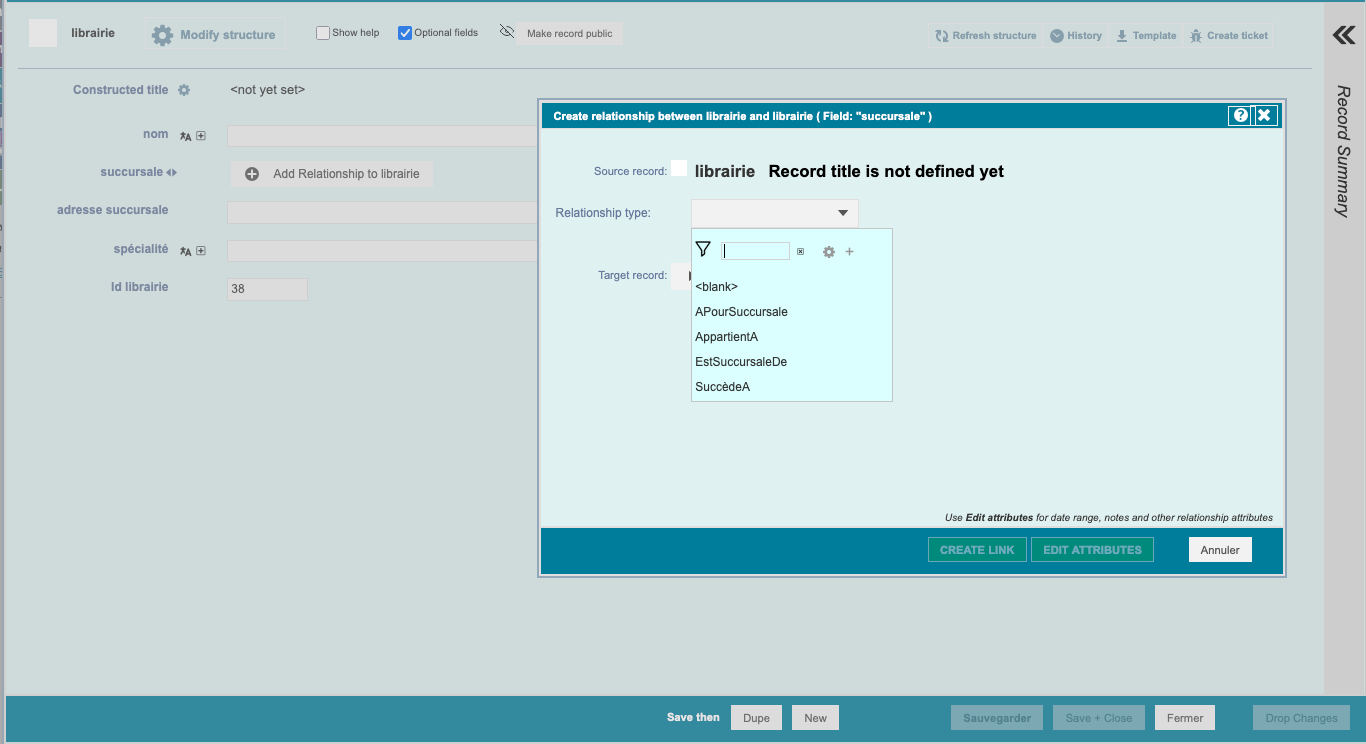
\includegraphics[width = 15cm]{Images/librairiesuccursale.png}
    \caption{Champ \enquote{succursale} dans le \emph{Record type} \enquote{librairie}. }
    \label{fig:champ-succursale}
\end{figure}

Le deuxième, appelé \enquote{lieu}, sert à distinguer les différents lieux occupés par les librairies. Il est surtout utile en cas de déménagement d'une librairie, phénomène fréquemment relevé dans les factures Rondel. 
L'intérêt est de pouvoir dater l'appartenance d'un lieu à un établissement grâce au champ \enquote{librairie}. Toujours grâce au vocabulaire contrôlé \enquote{RelationsLibrairies}, ce champ nous permet de lier notre enregistrement \enquote{lieu} à un enregistrement \enquote{librairie} pour une période donnée, grâce au terme \enquote{AppartientA}, et en soumettant cette relation d'appartenance à des bornes chronologiques, ce qui est l'un des intérêts des \emph{Relationship markers}. 

\begin{figure}[htbp]
    \centering
   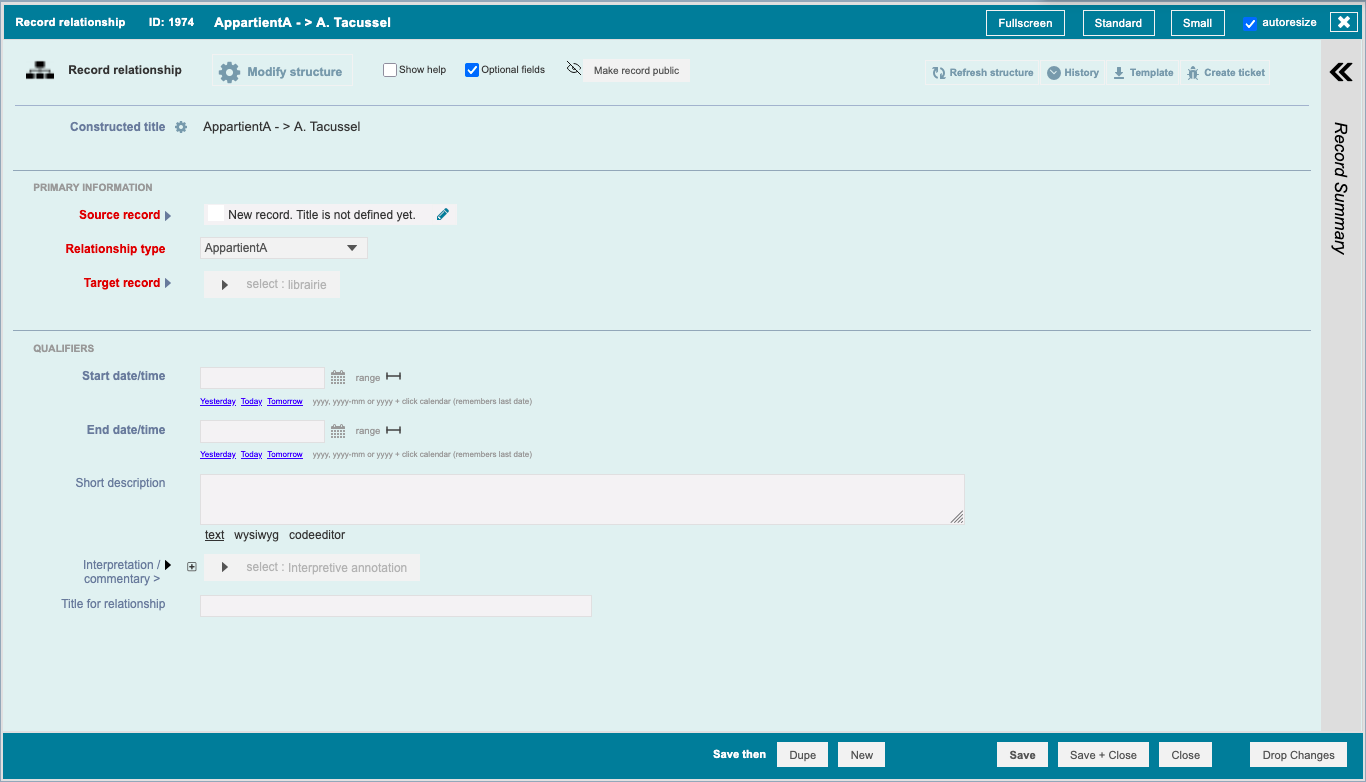
\includegraphics[width=15cm]{Images/Lieu.png}
    \caption{Remplissage du champ \enquote{librairie} de la table \enquote{lieu}.}
    \label{fig:champ-lieu-librairie}
\end{figure}

Les autres champs de ce \emph{Record type} permettent de situer les lieux spatialement. En voici deux exemples : 

Les champs \enquote{ville} et \enquote{pays}, sont tous les deux des choix déroulants parmi des vocabulaires contrôlés, constitués de listes de tous les pays et villes rencontrés dans les factures Rondel. Ces listes de lieux ne sont pas exhaustives, et seront amenées à être enrichies par les nouvelles villes et les nouveaux pays rencontrés dans le reste du corpus. 


Comme prévu, un \emph{Record type} de cette base, appelé \enquote{personne}, est avant tout conçu pour transcrire les informations concernant des personnes et issues des factures.
La plupart des champs servent à accueillir des informations assez sommaires trouvables dans les factures, telles que leurs noms, prénoms et professions (libraires le plus souvent). Grâce à un lien de type \emph{Record pointer}, chaque personne recensée est liée à l'établissement où elle travaille. Un champ de ce \emph{Record type}, appelé \enquote{PersonneAssociée}, permet d'indiquer des liens de différentes natures entre les personnes. Ce champ s'appuie encore sur un vocabulaire contrôlé, nommé \enquote{LiensEntrePersonnes}, et réalisé à partir des liens interpersonnels observés dans les factures. Ce vocabulaire définit d'abord le lien le plus évident que l'on peut percevoir dans les factures : les liens professionnels entre les personnes. 

\begin{figure}[htbp]
    \centering
    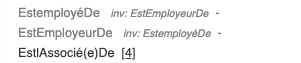
\includegraphics[width=10cm]{Images/LiensPro.png}
    \caption{Exemple de vocabulaire consacré aux liens professionnels entre les personnes}
    \label{fig:liens-professionnels}
\end{figure}

L'image ci-dessus montre les deux types de liens professionnels que nous avons modélisés : un lien \enquote{EstEmployeurDe}, lui aussi réciproque, dont le lien inverse est \enquote{EstEmployéDe}, et un lien plus simple, utilisé lorsque deux personnes travaillent ensemble sans lien de subordination visible, appelé \enquote{EstAssocié(e)De}. 

Les établissements étant souvent tenus par des familles de libraires, nous avons également décrit avec précision les différents types de liens familiaux susceptibles d'apparaître dans les factures. Pour ce faire, nous nous sommes inspirés d'un vocabulaire contrôlé déjà existant dans \emph{Heurist}\index{Heurist}, le vocabulaire \enquote{Family}, issu du groupe \enquote{Relationships}, qui représente tous les types de relations familiales pouvant exister. 

\begin{figure}[htbp]
    \centering
    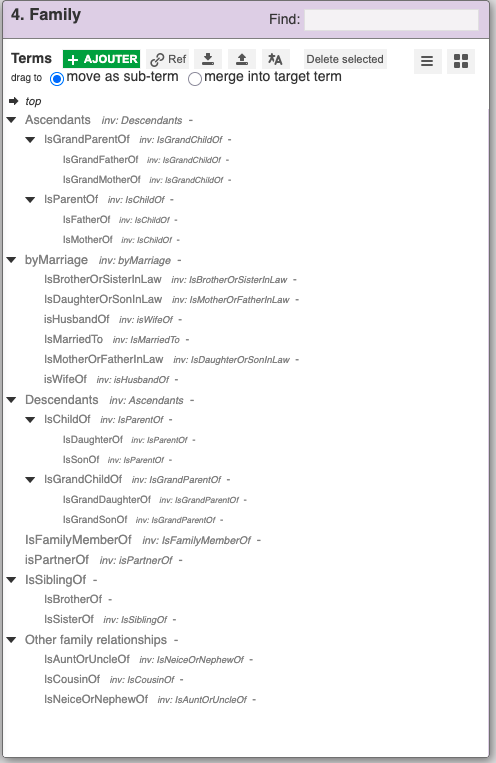
\includegraphics[width=7cm]{Images/family.png}
    \caption{Vocabulaire \enquote{Family}}
    \label{fig:vocabulaire-family}
\end{figure}
  
\begin{figure}[htbp]
    \centering
    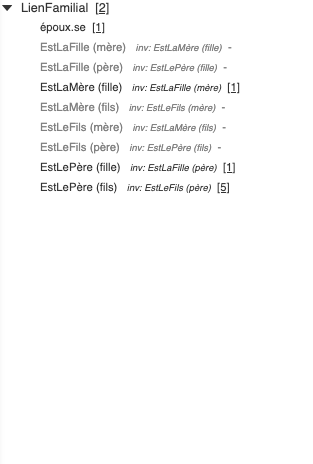
\includegraphics[width=7cm]{Images/LiensFamiliaux.png}
    \caption{Liens familiaux}
    \label{fig:liens-familiaux}
\end{figure}


\vspace{1.5cm}

Dans notre base de données, nous avons également représenté des liens réciproques, et en étant le plus précis possible, comme le montre l'image ci-dessous. 

\newpage
Le \emph{Record type} le plus important de cette base, et qui a vocation a être le plus fourni est sans aucun doute \enquote{ligne de facture}, ayant pour but de recenser chaque titre acheté par Rondel auprès d'une librairie. Cette table vise à répondre à l'un des objectifs principaux de ce travail, à savoir de retracer la provenance des oeuvres de la collection Rondel. Une partie des champs de cette table, spécialement dédiée à la transcription des factures, prévoit donc la possibilité de saisir tous types d'informations que nous avons relevées dans ces lignes, et qui concernent les oeuvres achetées. 

\begin{figure}[htbp]
    \centering
    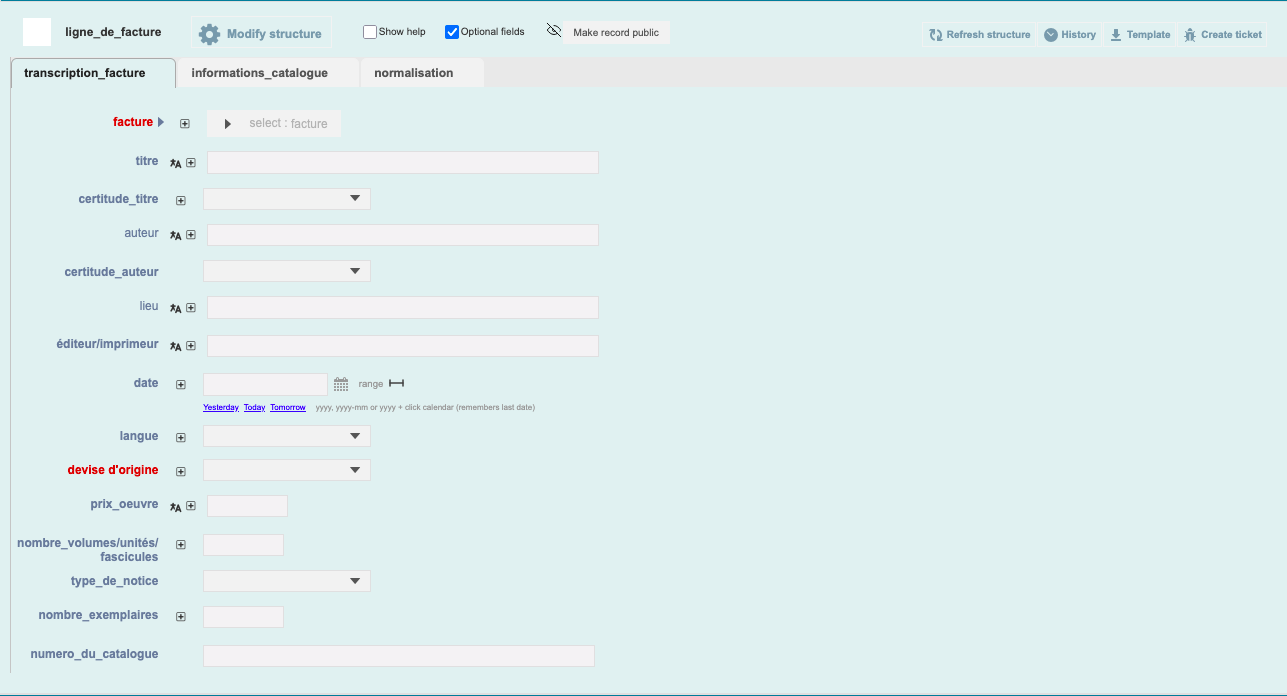
\includegraphics[width=12cm, height=8cm]{Images/transcription ligne facture.png}
    \caption{Champs de la table \enquote{ligne de facture} prévus pour les informations directement transcrites des factures.}
    \label{fig:champs-ligne-facture}
\end{figure}

Comme on peut le constater sur le formulaire de saisie ci-dessous, les champs concernent des informations variées, allant du plus évident et indispensable pour retrouver une oeuvre (titre, auteur, date, ...) à des informations plus précises, que l'on ne peut trouver que dans certaines factures (éditeur/imprimeur, lieu, ou encore le numéro qui identifie l'oeuvre dans les catalogues des libraires, ...). Peuvent aussi être renseignés les prix des oeuvres et leurs devises, qui encore une fois font l'objet d'un vocabulaire contrôlé. 
On peut voir que les champs obligatoires de cette table (en rouge) sont très rares, comparés aux champs dits \enquote{recommandés}, qui sont majoritaires. Nous avons fait ce choix car le niveau d'information dans les factures est, nous l'avons dit, très hétérogène. Le but est que le manque de données sur la facture ne devienne jamais un obstacle pour en saisir les informations dans la base.  

\vspace{1.5cm}
Afin de pouvoir remonter à la source des informations, chaque enregistrement \enquote{ligne de facture} est lié à un  autre enregistrement, saisi au préalable, de type \enquote{facture}. Il s'agit du cinquième et dernier \emph{Record type} qui compose cette base, et son rôle est d'indexer chaque facture, et de renseigner les informations principales la concernant, et utiles pour la retrouver. On trouve donc l'établissement producteur de la facture ainsi que sa date, mais aussi la cote du dossier où elle est rangée, ce qui n'est pas forcément indispensable car, nous l'avons vu, chaque dossier est en général consacré à un libraire, mais peut toujours être utile dans certains cas. Au-delà de ces informations essentielles, cette table recense aussi toutes les données qui concernent directement la facture, à savoir le nombre de titres qui la compose, son montant et les frais souvent inclus  (frais de port, ...), ou encore la devise dans laquelle le paiement est fait (reposant sur le même vocabulaire contrôlé que pour la table précédente).

Ces deux dernières tables correspondent donc à deux échelles d'information venant des factures : l'une à une échelle très large, celle des factures, relevant plutôt de l'analyse du document en lui-même et de sa structure, et l'autre à l'échelle de la ligne de facture qui, beaucoup plus précise, répond directement à l'objectif d'identification des titres achetés. 


\newpage

\section{La saisie de données}

La saisie manuelle de données est une pratique nécessaire à l'enrichissement et à l'évolution de cette base de données. Elle demeure en effet le moyen privilégié pour transcrire les données des factures à la base. Plus qu'un moyen, la saisie est également la meilleure façon de connaître intimiment les sources sur lesquelles on travaille, et suscite inévitablement des nouveaux questionnements\footcite{Lemercier_Zalc_2008}. L'étape de saisie de données est donc essentielle, car elle permet d'éprouver le modèle que nous avons conçu, et de le faire évoluer en fonction de ce qu'on rencontre dans les sources, dans le but, à terme, de le stabiliser. 
La saisie au sein de cette base a été pensée selon des bonnes pratiques à respecter\footcite[Voir les dix commandements  de la saisie]{Lemercier_Zalc_2008}. Nous avons par exemple accordé une attention particulière au fait de conserver avec précision l'orthographe de la source, et de ne l'avoir modernisée qu'\emph{a posteriori}, dans des champs spécifiques de la base. Les informations ajoutées, extérieures à la source, sont donc  séparées nettement de celles issues des factures. 
L'étape de saisie pourra être réalisée par des conservateurs, des chercheurs, et quiconque utilisera la base. Pour cela, une documentation détaillant tous les usages ultérieurs possibles de la base, et destinée aux futurs utilisateurs explique entre autres, champ par champ, comment saisir manuellement les informations dans la base\footnote{Un renvoi vers cette annexe sera fait ici quand celle-ci sera finalisée}. 

Ainsi, la saisie de données est la façon la plus évidente d'envisager le traitement informatique de ce corpus, mais aussi d'enrichir la réflexion sur ce que peuvent nous dire ces factures. Cette pratique doit donc être particulièrement fléchée et encadrée. 


\section{Limites d'\emph{Heurist}}


Les objectifs et la portée de ce projet doivent aussi être définis en gardant en tête qu'Heurist est limité sur de nombreux aspects. 
Les limites d'\emph{Heurist}\index{Heurist} concernent à la fois son fonctionnement général et certains aspects techniques plus précis. 

De manière générale, le principal défaut d'\emph{Heurist}\index{Heurist} est le manque de documentation à son sujet, et le fait que la documentation ne soit pas assez actualisée. Il existe une documentation officielle en anglais sur \emph{Heurist}, mais celle-ci peut être difficile à appréhender\footcite{heurist_help}. La documentation française, quant à elle, est très dispersée, et se présente sous la forme de tutoriels réalisés par différentes institutions, comme par exemple Huma-Num, qui héberge le logiciel\footcite{huma-num_heurist_2026}. Une autre difficulté liée à cette documentation est que le logiciel est régulièrement actualisé, et que la documentation ne l'est pas systématiquement. Par conséquent, elle ne correspond pas toujours à ce que l'on trouve actuellement dans le logiciel, ce qui peut être déroutant. Pour compenser cela, la liste de diffusion officielle gérée par la communauté d'utilisateurs, très active, d'\emph{Heurist}, nous a permis de nous tenir au courant de l'actualité du logiciel et même à poser des questions en cas de difficulté\footcite{noauthor_heurist-utilisateurs_nodate}. 

La forme d'\emph{Heurist}\index{Heurist} fait que nous avons également été limités dans nos possibilités techniques, c'est pourquoi nous avons dû utiliser des moyens détournés pour parvenir à mettre en oeuvres certaines fonctionnalités de notre base de données. Par exemple, Heurist\index{Heurist} n'a pas un type de données spécialement dédié aux booléens, c'est-à-dire aux réponses par \enquote{oui} ou par \enquote{non}. Ce type de données est pourtant assez classique, et très courant dans les jeux et les bases de données. \emph{Heurist}\index{Heurist} prévoit malgré tout l'utilisation de ce type de données de manière détournée. En effet, certains vocabulaires contrôlés qui pré-existaient à notre base jouent le rôle des booléens. C'est le cas, au sein du groupe de vocabulaires \enquote{Categorisation and flags}, de deux vocabulaires nommés \enquote{Flag}, dont l'un contient \enquote{Yes} et \enquote{No}, et l'autre \enquote{Yes}, \enquote{No} et \enquote{Unknown}. Ils peuvent donc être utilisés comme des vocabulaires contrôlés classiques, et exprimer un choix entre oui et non. Il faut noter qu'il est tout à fait possible de créer son propre vocabulaire contrôlé composé des options \enquote{oui} et \enquote{non}, dans n'importe quelle langue. 
Le fait de pouvoir choisir des niveaux de certitude des informations pour les données en format \enquote{date} a été beaucoup apprécié dans l'utilisation du logiciel. Cependant, il aurait été plus adapté aux objectifs de notre projet que cette option n'existe pas que pour les dates, et soit disponible pour d'autres types de données. En effet, nous étions obligés de rentrer des informations hypothétiques dans la base lorsque nous n'étions pas sûr de l'orthographe d'un mot où de l'exactitude d'un intitulé écrit sur une facture. Pour pallier à cela, nous avons créé des champs dédiés pour les informations essentielles de la base : des champs \enquote{certitude titre} et \enquote{certitude auteur}, constitués des options \enquote{oui} et \enquote{non}. 

\vspace{1.5cm}

Ainsi peut-on résumer l'exploitation d'un maximum de données des factures Rondel et leur retranscription dans la base \emph{Heurist}\index{Heurist}. Il convient maintenant de s'intéresser à tous les traitements que ce logiciel nous permet de réaliser à partir de ces données, qu'il s'agisse d'enrichissements ou de visualisations. 
\chapter{La base de données comme réponse à des besoins : datavisualisations, enrichissements et possibilités offertes par ce projet}

Comme nous l'avons évoqué, \emph{Heurist}\index{Heurist} est utilisé pour sa capacité à satisfaire de nombreux besoins, auxquels notre travail a pour but de répondre. 

\section{Enrichissements de la base par des informations extérieures aux factures}

Si le besoin essentiel auquel doit répondre la base est, nous l'avons vu, de transcrire les factures, elle doit aussi prévoir la possibilité d'être complétée par des informations venues de sources extérieures.
L'utilité principale est de nous renseigner davantage sur ce que l'on recherche dans la base si les seules informations présentes dans les factures sont lacunaires. C'est pourquoi une partie des champs du \emph{Record type} \enquote{ligne de facture} sert à accueillir des données issues des catalogues en ligne de la BnF contenant les oeuvres de la collection Rondel, à savoir le catalogue général\index{Catalogue général de la BnF} ou BnF Archives et Manuscrits\index{Bnf Archives et manuscrits}. 

\begin{figure}[htbp]
    \centering
    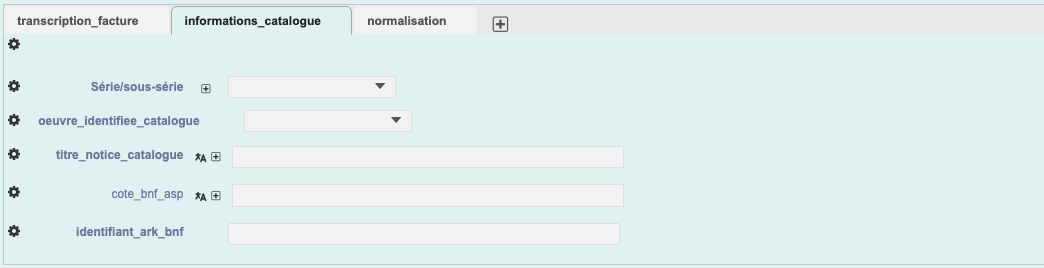
\includegraphics[width=12cm]{Images/informations catalogue_2.png}
    \caption{Section \enquote{Informations catalogue} dans le \emph{Record type} \enquote{ligne de facture}.}
    \label{fig:informations-catalogue}
\end{figure}

\newpage
Comme nous le montre l'image ci-dessus, \emph{Heurist}\index{Heurist} permet de diviser chaque \emph{Record type} en plusieurs sections, appelées \emph{Tabs}. Grâce à cela, nous avons pu distinguer clairement dans une \emph{Tab} appelée \enquote{transcription factures} les données issues des factures, et dans une autre nommée \enquote{informations catalogues} celles trouvées dans les catalogues de la BnF, car comme nous l'avons vu, il est essentiel dans la saisie de données d'indiquer l'origine des informations. Ces champs sont très importants dans notre travail, parce qu'ils permettent de retrouver, dans les catalogues de la BnF, les oeuvres indiquées dans les factures, et de faire un lien entre les deux. En effet, un champ est prévu pour indiquer la cote de l'ouvrage au sein de la collection, lorsque celle-ci est clairement identifiée. Un autre champ permet de sélectionner la série et/ou la sous-série à laquelle l'oeuvre appartient à l'aide d'un vocabulaire renseignant le nom de cet ensemble, et l'intervalle de cote associé, pour pouvoir l'associer à l'oeuvre avec certitude. 

\begin{figure}[htbp]
    \centering
    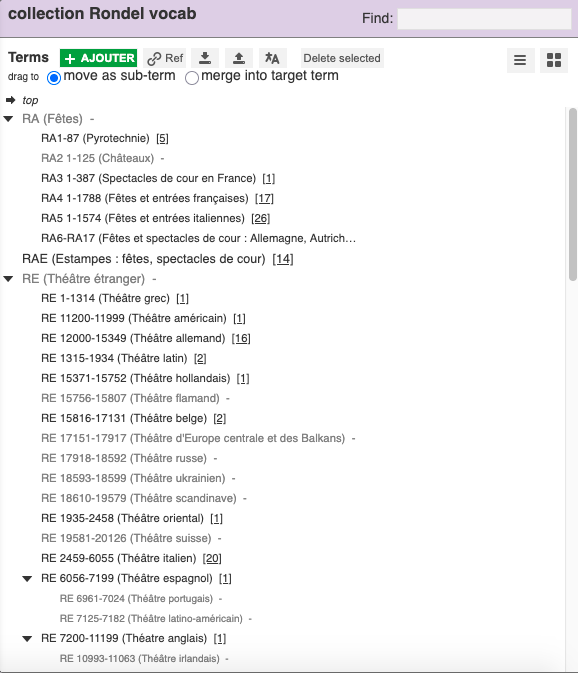
\includegraphics[width=12cm]{Images/collec_Rondel_vocab.png}
    \caption{Vocabulaire contrôlé qui recense les différentes séries et sous-séries de la collection Rondel, et leurs intervalles de cotes respectifs.}
    \label{fig:vocabulaire-collection-rondel}
\end{figure}
\newpage


Il est donc parfois possible, en complétant avec des informations venant des catalogues, de retrouver avec précision la provenance d'un exemplaire de la collection Rondel.

Ce principe de champs spécialement prévus pour les ajouts d'informations extérieures, à bien séparer dans des sections distinctes de ce qui provient des factures, a également été utilisé dans la table \enquote{personne} de notre base, cette fois pour donner la possibilité d'approfondir la recherche sur des personnes. Cela entend répondre au besoin, identifié lors du travail préparatoire à la modélisation, de s'intéresser plutôt aux libraires. Ces champs, non obligatoires, n'ont pas vocation à être remplis systématiquement lorsqu'on saisit une personne dans la base, mais anticipent plutôt des potentiels usages prosopographiques sur des libraires. Ainsi, nous avons ajouté dans la table \enquote{personne} une section \enquote{enrichissements}, notamment constituée des dates de naissance et de mort des personnes, et des champs voués à l'ajout d'informations biographiques et à l'indication des sources utilisées.
Afin d'expérimenter ces champs, mais également d'autres possibilités offertes par la base, nous avons décidé de sortir de l'échantillon que nous utilisions au départ, et de mener nous-mêmes des recherches approfondies sur un ou des libraires en particulier. Cela nous a amené à nous intéresser à la famille Saffroy, une grande famille de libraires ayant exercé son activité à Paris et au Pré-Saint-Gervais entre 1880 et 2020\footcite{magazine_famille_2021}. Nous avons découvert cette famille en examinant les titres des dossiers qui composent notre corpus, et en remarquant qu'Auguste Rondel a été client de plusieurs membres de cette famille\footnote{Les dossiers concernant la famille Saffroy sont dans le catalogue BnF Archives et Manuscrits sous les cotes RCOL-1(382) à (386).}. Notre recherche s'est donc focalisée sur cette famille, et nous avons renseigné dans la base tous ses membres qui apparaissent dans les factures, leurs proches, et les liens qui les unissent. 

En somme, si cette base garde pour fonction principale d'accueillir un maximum d'informations des factures, elle a pour visée secondaire de permettre l'ajout d'informations extérieures, pour la compléter et approfondir les recherches. Cependant, il doit être possible d'identifier clairement la source de toutes les données présentes dans la base. 

\newpage 
\section{Interopérabilité, liens avec d'autres logiciels et réutilisation des données}

Cette base de données entend exploiter les possibilités d'\emph{Heurist} pour répondre, dans la mesure du possible, à des enjeux essentiels dans les projets de recherche : la conformité aux objectifs de la science ouverte et le respect des principes FAIR (\emph{Findable}, \emph{Accessible}, \emph{Interoperable}, \emph{Reusable}). 

Pour ce faire, l'enrichissement de la base avec des informations extérieures peut servir à y intégrer  des formats interopérables, en liant les données à des concepts universels et identifiés de manière unique sur le web. L'enjeu est de se rapprocher de l'ambition portée par le web de données. Théorisé dès 1998 sur la feuille de route pour le web sémantique de Tim Berners-Lee par l'expression \emph{Web of data}, le web de données est une vision du web proposant une interopérabilité fondée sur la création d'un espace global d'information où toutes les données sont liées entre elles, et sont compréhensibles par les machines\footcite{bermes_2_2013}. C'est pourquoi l'un des champs de la section \enquote{informations catalogue}, appelé \enquote{identifiant ark bnf}, est prévu pour accueillir l'identifiant ARK associé à chaque oeuvre identifiée dans le catalogue. De même, la section \enquote{enrichissements} de la table \emph{personne}, présentée dans la partie précédente, contient un champ appelé \enquote{notice autorité} prévue pour indiquer, s'il existe, l'identifiant ARK de l'autorité BnF de la personne que l'on saisit. 
L'\emph{Archival Resource Key} est un système fournissant des URL stables pour les ressources numériques, utilisé dans les institutions patrimoniales, et notamment dans les bibliothèques\footcite[p. 34]{hervieu_2024}. L'ARK est un identifiant pérenne faisant partie des données d'autorité qui contrôlent la description des ressources de la BnF, c'est pourquoi il est nécessaire de pouvoir s'y référer depuis notre base de données\footcite{noauthor_donnees_nodate}. 

Dans ce même but, tous les noms de lieux associés à des librairies sont indexés dans des formats interopérables, afin d'être rattachés à des standards universels, à des référentiels exposés sur le web\footcite[Voir \enquote{Présentation de Heurist}]{paillusson_introduction_2022}. Cette possibilité est offerte par les vocabulaires contrôlés d'\emph{Heurist}\index{Heurist}, dont les termes peuvent être associés à une URI cliquable. Ainsi, les noms de villes et de pays indexés dans notre base sont tous reliés à des identifiants \emph{GeoNames}\index{GeoNames}, une base de données géographique mondiale recouvrant plus d'onze millions de lieux\footcite{noauthor_geonames_nodate}. 

\begin{figure}[htbp]
    \centering
    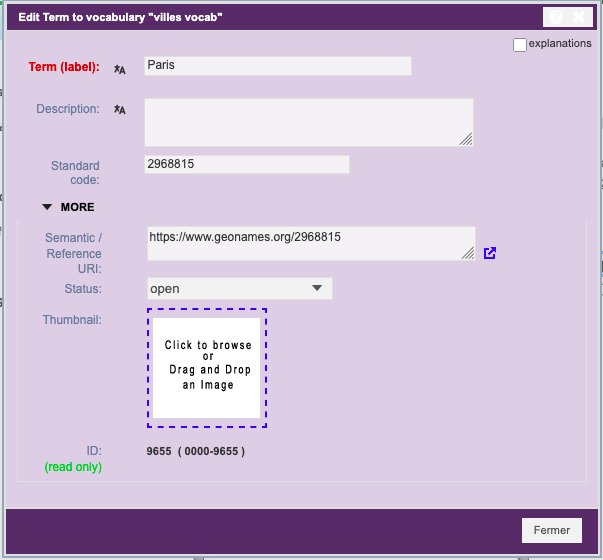
\includegraphics[width=12cm]{Images/lieux_web_semantique.png}
    \caption{ville de Paris identifiée dans la base et liée à \emph{GeoNames} conformément aux principes de mise à disposition des données dans le cadre du web sémantique (ces identifiants sont exprimés par des URI, et formulés grâce au protocole HTTP, pour qu'on puisse y accéder).}
    \label{fig:paris-geonames}
\end{figure}



\newpage


La compatibilité avec d'autres logiciels peut également servir à enrichir rapidement et automatiquement une base par l'import de données du web. Ce besoin est notamment assuré par la fonction de synchronisation entre \emph{Heurist}\index{Heurist} et \emph{Zotero}\index{Zotero}, un logiciel libre, gratuit et simple d'utilisation permettant de collecter, d'organiser, d'annoter, de citer et de partager des ressources bibliographiques\footcite{noauthor_zotero_nodate}. 
La synchronisation possible entre les deux logiciels permet donc d'importer, dans une base \emph{Heurist}\index{Heurist}, des notices bibliographiques complètes et générées avec \emph{Zotero}\index{Zotero}. Cette opération est possible grâce à une clé API, et à un identifiant appelé \emph{User ID}, qu'il nécessaire de récupérer sur le site zotero.org. Ces identifiants sont à renseigner ensuite dans \emph{Heurist}\index{Heurist}, en suivant des étapes énumérées dans le guide sur les usages de la base\footnote{Voir à la page 16 de l'annexe C - I. \enquote{ \nameref{documentation}}}. Dès lors, la synchronisation entre les deux logiciels se fait immédiatement, et peut être mise à jour à tout moment en appuyant simplement à nouveau sur le bouton dédié. Les données issues de \emph{Zotero}\index{Zotero} apparaissent dans des enregistrements spécifiques, chacun étant consacré à une ressource. Cette possibilité sert à enrichir rapidement une base de données avec tous types d'informations issues du web, ou de sourcer plus facilement les informations de la base. Il s'agit aussi d'une preuve supplémentaire de la pertinence d'\emph{Heurist} dans les projets en sciences humaines, car le logiciel est compatible avec d'autres outils courammment utilisés dans la recherche. 
Cependant, cette synchronisation présente des limites. En effet, il n'est pas possible de contrôler l'endroit où vont les données de \emph{Zotero}, en prévoyant des champs adéquats dans la base. Les données ne sont pas visibles directement au sein des \emph{Record types}, mais sont classés par types de ressources (\emph{Book}, \emph{Web Bookmark}, ...). Pour les faire apparaître dans la base, nous avons donc créé un champ au sein de la table \enquote{personne} faisant le lien entre une personne et une ressource Zotero\index{Zotero}. Cet exemple montre une autre façon d'associer, à une base Heurist\index{Heurist}, des données du web.  

En plus de pouvoir être liées à des standards universels et d'être intégrées au web, les données \emph{Heurist}\index{Heurist} sont exportables dans des formats ouverts, et réutilisables dans de nombreux autres logiciels. Elles peuvent par exemple être exportées en CSV, XML ou JSON, mais également être importées dans \emph{Heurist}\index{Heurist} dans les mêmes formats\footcite[Voir \enquote{Présentation de Heurist}]{paillusson_introduction_2022}. Cette réutilisation possible des données a également répondu aux besoins de notre projet, car certains traitements que nous souhaitions réaliser étaient impossibles avec \emph{Heurist}\index{Heurist}. Le logiciel ne permet pas de réaliser des calculs précis. Or, la base de données a aussi parmi ses objectifs de nous renseigner sur les dépenses effectuées par Auguste Rondel dans sa collection. Cela explique pourquoi plusieurs champs du \emph{Record type} \enquote{facture} sont consacrés aux prix totaux, aux frais et aux devises renseignés dans les factures. Nous avons donc exporté cette table en format CSV afin de pouvoir réaliser les calculs dont nous avions besoin grâce à des formules Excel\index{Excel}. Les formules étaient très simples : il s'agissait de multiplications, dans le but de convertir en francs tous les prix totaux et les frais payés par Auguste Rondel. Les conversions ont été effectuées depuis toutes les monnaies que nous avions dans l'échantillon (franc suisse, lire, livre, mark et Reischmark), et grâce à un taux de change déterminé avec l'outil currency converter de Historical statistics\footcite{noauthor_historical_nodate}. Une fois ces calculs faits, nous avons importé le fichier CSV avec tous les prix normalisés en franc dans la base. Tout ce procédé, dont il ne faut pas oublier les biais et le caractère expérimental, est lui aussi détaillé dans la documentation sur les usages ultérieurs de la base\footnote{Voir \enquote{ \nameref{documentation}}}. Il convient surtout de retenir de cet exemple que les données \emph{Heurist}\index{Heurist} peuvent facilement être exportées et importées dans des formats ouverts, ce qui permet de les réutiliser dans d'autres cadres, au-delà du logiciel lui-même. 

\section{Requêtes et visualisations possibles à partir de la base}

Après nous être intéressés à l'intégration de données extérieures dans la base, et aux besoins auxquels nous tentons de répondre en matière de science ouverte, il convient de nous pencher sur les différents moyens d'interroger les données et les visualiser. 

\vspace{1.5cm}

L'un des intérêts d'une base de données relationnelles est de pouvoir interroger ses données. Cela fait partie des raisons de l'utilisation d'une base de données dans notre projet, car la finalité de collecter autant de données issues des factures est de pouvoir les interroger, les manipuler, se focaliser sur certains aspects, dans le but d'en extraire des statistiques, de les visualiser ou encore de les publier. Dans la plupart des SGBDR (Système de gestion de bases de données relationnelles), l'interrogation des tables d'une base se fait, comme nous l'avons vu dans le chapitre 3, grâce au langage SQL. Cependant, comme l'utilisation de notre base se veut être accessible à un public large, il est nécessaire de pouvoir interroger la base sans avoir à coder. Pour cela, \emph{Heurist} prévoit plusieurs manières d'interroger un ou plusieurs \enquote{Record types}. 
Tout d'abord, chaque table peut être interrogée séparément par des filtres. Il suffit d'utiliser le mode \emph{Explore}, et de créer un filtre grâce à l'icône représentant un entonnoir. Le filtre permet de ne sélectionner, au sein d'une table, que les enregistrements répondant à certains critères. Il est également possible d'enregistrer les filtres créés, et de les conserver ensemble grâce à la rubrique \emph{Saved filters}. Une fois les filtres enregistrés, on peut accéder à la requête produite par \emph{Heurist} à partir de ce qu'on a sélectionné. 
Ces filtres sont l'équivalent des requêtes SELECT en SQL, qui permettent d'extraire d'une base de données les données répondant à des questions que l'on peut se poser\footcite[p. 203]{Hainaut_2015}. 
Cette fonctionnalité d'\emph{Heurist} est très adaptée à notre projet de recherche, car celui-ci entend pouvoir se focaliser sur des thématiques particulières, comme par exemple une typologie de documents, ou un libraire en particulier. Les images ci-dessous montre les requêtes issues de plusieurs filtres réalisés dans le cadre de notre travail. 

\begin{figure}[htbp]
    \centering
    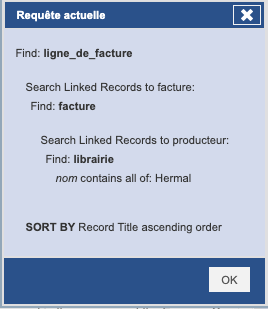
\includegraphics[width=5cm]{Images/requete_Hermal.png}
    \caption{Cette requête sélectionne, dans la table \enquote{ligne de facture}, toutes les lignes liées à un enregistrement \enquote{facture}, eux-mêmes liés à un  enregistrement \enquote{librairie} qui contient le mot \enquote{Hermal}, et trie les titres par ordre alphabétique. En somme, elle ne sélectionne que les documents achetés par Rondel à la librairie Hermal.}
    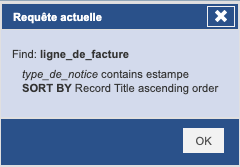
\includegraphics[width=5cm]{Images/requete_estampes.png}
    \caption{Cette requête sélectionne toutes les lignes de facture dont le champ \enquote{type de notice} contient le terme \enquote{estampe}, et trie les titres par ordre alphabétique. Elle ne sélectionne donc que les estampes.}
    \label{fig:requetes-heurist}
\end{figure}

Cependant, les possibilités de requêtes dans \emph{Heurist} sont très limitées par rapport à celles du langage SQL. Par exemple, les filtres du logiciel ne permettent pas d'interroger plusieurs tables en une seule requête, comme le font les jointures (\emph{join}) en SQL\footcite[p. 228]{Hainaut_2015}. 

Pour faciliter l'interrogation de la base, nous avons surtout opté pour la deuxième possibilité offerte par \emph{Heurist}\index{Heurist}, à savoir les \emph{Faceted search}, ou \enquote{filtres à facettes}. Il s'agit d'un mode de navigation structurée permettant de filtrer une recherche dans la base à l'aide de nombreux critères, correspondant aux différents champs de la base et pouvant prendre la forme de recherche plein texte, de listes de sélection ou encore de cases à cocher\footcite[\enquote{Création d’un filtre de recherche à facettes}]{paillusson_introduction_2022}. Sorte de recherche avancée au sein d'une base Heurist\index{Heurist}, les facettes permettent de se concentrer plus précisément sur certaines propriétés d'une ou plusieurs tables\footcite[Filter-Edit-Analyse-Publish]{noauthor_faceted_nodate}. 

\begin{figure}[htbp]
    \centering
    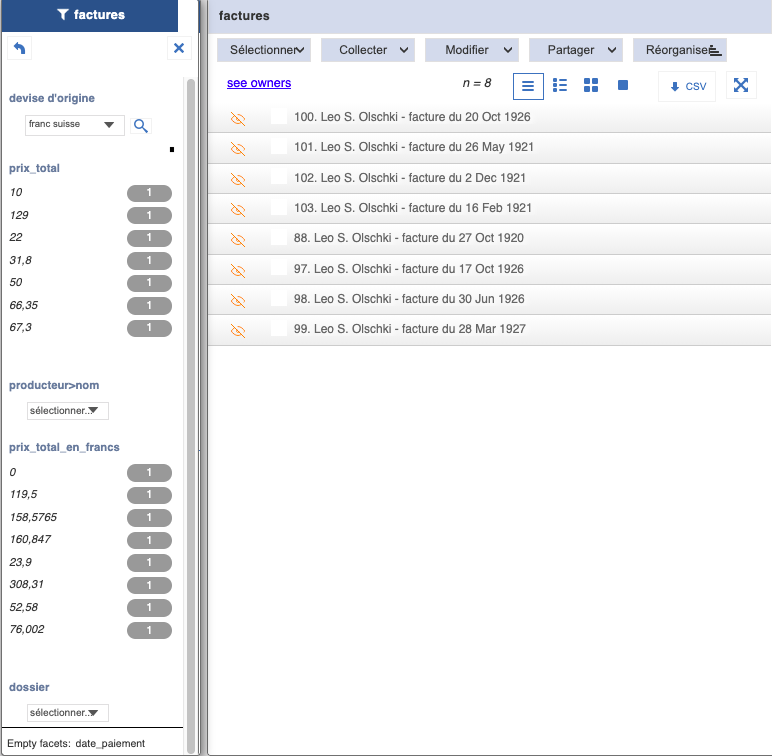
\includegraphics[width=15cm]{Images/facet_factures.png}
    \caption{Recherche à facettes sur la table \enquote{facture}, qui n'interroge ici que les factures payées en francs suisses.}
    \label{fig:facettes-factures}
\end{figure}

Dans ce projet, les facettes sont privilégiées aux filtres, car elles ressemblent davantage aux formes de recherches avancées que l'on peut trouver habituellement dans les catalogues de bibliothèques ou sur d'autres sites internet. Elles paraissent donc plus simples à prendre en main par un public large. 

Comme nous l'avons vu, interroger cette base de données nous permet de répondre à certains enjeux du projet de recherche en cours, en se focalisant sur certains de ses aspects en particulier. L'interrogation des données doit être comprise conjointement à leur visualisation, car les données sont souvent interrogées dans le but d'être visualisées. 

\vspace{1.5cm}

La datavisualisation se définit par sa capacité à présenter rapidement les données et à les rendre lisibles\footcite[p. 11]{lagnel_2021}. Elle est une attente majeure de ce projet, car cela matérialise ce que nous disent les factures Rondel sur tous les sujets qu'elles permettent d'étudier. Il s'agit de l'un des intérêts d'\emph{Heurist}\index{Heurist} qui, nous l'avons évoqué, est pensé pour répondre aux problématiques des SHS, intégrant donc nativement diverses possibilités de visualisation\footcite[\enquote{Présentation de Heurist}]{paillusson_introduction_2022}. Notre projet de recherche a donc produit différents types de visualisations en lien avec les questions qu'il entend traiter. 

Conformément aux objectifs du projet, les factures Rondel peuvent largement être exploitées pour étudier les réseaux de libraires. Le logiciel est très utile par sa capacité à créer des graphes, de manière à représenter les relations de la base sous forme de réseau. La visualisation du réseau standard est constitué de noeuds (points), et d'arêtes (ligne qui les relie)\footcite[p. 189]{Drucker_2020}. C'est le principe de la fonction \emph{Network}, au sein du mode \emph{Explore} du logiciel, qui affiche sous la forme d'un réseau toutes les relations enregistrées dans une table. Dans le chapitre 5, nous avons vu que l'exploitation des factures a permis de saisir et de caractériser de manière précise de nombreuses relations entre des personnes ou des libraires indexées dans la base\footnote{Voir p.\pageref{conception base}}. Toutes ces relations sont donc modélisables sous forme de graphes, et visibles directement dans \emph{Heurist}\index{Heurist}. Les réseaux créés à partir de la base sont visibles et expliqués dans les annexes\footnote{Voir dans l'annexe D, \enquote{ \nameref{reseaux heurist}}.}. 
La visualisation de réseaux est, nous l'avons vu, disponible nativement avec \emph{Heurist}. Cependant, il est également possible, si l'on souhaite approfondir cette question, d'exporter les données concernées en un fichier de graphe au format .gexf, et de visualiser les réseaux grâce au logiciel gephi\index{Gephi}. Ce logiciel permet d'explorer, de manipuler et de comprendre des réseaux complexes\footcite{noauthor_gephi_nodate}, et a été expérimenté dans le cadre de ce travail sur l'ensemble des relations de la table \enquote{personne}\footnote{Voir l'annexe \enquote{\nameref{reseau gephi}}.}.


Les données issues des factures permettent aussi d'étudier spatialement les librairies où Rondel s'est fourni. En effet, il est possible d'utiliser \emph{OpenStreetMap}\index{OpenStreetMap} au sein même de la base \emph{Heurist}\index{Heurist}, afin de produire des visualisations cartographiques. Le principe est simple : il suffit de créer un champ de type \emph{geospatial} afin d'y saisir des noms de lieux ou d'adresses, qui seront ensuite géoréférencés. La visualisation d'une carte montrant tous les lieux géoréférencés est alors permise par une autre fonction du mode \emph{Explore}, appelée \emph{Map}. Dans le cadre du projet de recherche sur les factures Rondel, cela permet, grâce à la création d'un champ \enquote{coordonnées géographiques} au sein de la table \enquote{lieu}, de produire une carte de tous les libraires où Auguste Rondel s'est fourni\footnote{Voir l'annexe \enquote{\nameref{cartes heurist}}.}. Dans ce cas précis, il peut être particulièrement intéressant de produire une carte à partir d'une requête, car l'un des enjeux du projet est, on le rappelle, de pouvoir se concentrer sur une thématique en particulier, comme une aire géographique. Ainsi, il est tout à fait possible, par un filtre, de n'afficher sur une carte que les librairies parisiennes par exemple. 

Comme les réseaux, les données cartographiques indexées peuvent être visualisées à l'intérieur même de la base \emph{Heurist}\index{Heurist}, mais peuvent aussi être exportées dans des formats spécifiques, pour exploiter les possibilités de logiciels plus spécialisés. Il est possible d'exporter ces données au format KML (\emph{Keyhole Markup Language}), format de données XML utilisé pour afficher des informations dans un contexte géographique\footcite{francois_kml_2017}. Nous avons utilisé l'autre possibilité, à savoir l'export en GeoJSON, format d'encodage de données géospatiales basé sur \emph{Javascript Object Notation} (JSON). Ce dernier nous a servi à exporter nos données géospatiales pour les réutiliser dans le logiciel QGIS\index{QGIS}, logiciel libre de système d'information géographique (SIG) permettant notamment de créer et d'annoter des cartes. Ce logiciel a surtout été utilisé pour tester l'export de données GeoJSON depuis \emph{Heurist}. Ce logiciel a donné la possibilité de récupérer toutes les données géospatiales de la table \enquote{lieu}, de les placer sur un fonds de carte \emph{OpenStreetMap}\index{OpenStreetMap}, et d'en créer un fichier PNG avec une légende\footnote{Voir l'annexe \enquote{\nameref{carte qgis}}.}. Ces fonctionnalités minimales de QGIS\index{QGIS} ont été utilisées à titre d'exemple, mais le logiciel offre de nombreuses autres possibilités à partir de données géospatiales. 


Ces pratiques cartographiques ont ouvert la voie à d'autres expérimentations, reposant également sur le principe de géoréférencement. Toujours dans le but de cartographier les librairies, y compris en se concentrant sur une aire géographique précise, nous avons expérimenté l'outil GALLIGEO\index{Galligeo}, qui permet, grâce au géoréférencement par points de contrôle, de produire une visualisation spatiale sur des cartes anciennes disponibles sur Gallica\index{Gallica}, bibliothèque numérique de la BnF\footcite[p. 27]{hervieu_2024}. Tout comme l'outil cartographique d'\emph{Heurist}, GALLIGEO\index{Galligeo} utilise une carte \emph{OpenStreetMap}\index{OpenStreetMap}, sur laquelle on peut renseigner les adresses une fois que la carte est géoréférencée. L'usage de cet outil pour exploiter les factures Rondel est complètement extérieure à toute utilisation d'\emph{Heurist}, mais peut servir à certaines études de cas. Par exemple, nous avons utilisé GALLIGEO\index{Galligeo} pour géoréférencer toutes les librairies marseillaises où Rondel s'est fourni, sur un fonds de carte datant de 1931\footnote{Voir l'annexe \enquote{\nameref{carte galligeo}}.}. Tout comme dans la base \emph{Heurist}\index{Heurist}, cette étude a permis de visualiser spatialement les librairies, mais en se rapprochant davantage des réalités de l'époque. 

\vspace{1.5cm}
Il faut noter que d'autres formes de datavisualisation sont possibles, mais qu'elles ont été experimentées de manière plus secondaire pour exploiter les données des factures Rondel. L'outil \emph{Crosstabs}, ou \emph{cross-tabulation}\footcite{noauthor_crosstabs_nodate}, permet de faire des calculs sur les données d'un \emph{Record type}, et d'en représenter les résultats sous forme de tableau, ou de graphique sectoriel, aussi appelé \emph{Pie chart} ou plus familièrement \enquote{camembert}. 
Cette fonction est accessible dans le mode \emph{Explore}, et pour l'utiliser, il suffit de sélectionner le \emph{Record type} et les champs concernés. 
Il serait très intéressant d'utiliser les \emph{Crosstabs} ultérieurement avec cette base, car cet outil permettrait de faire des statistiques sur la collection Auguste Rondel, ou sur la base de données en elle-même. Cependant, la base ne contient pas assez de données à ce stade pour que des statistiques soient représentatives. Nous avons malgré tout expérimenté cette possibilité à plusieurs reprises. En voici un exemple : 


\begin{figure}[htbp]
    \centering
    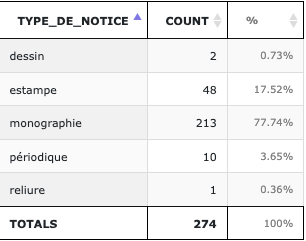
\includegraphics[width=0.5\textwidth]{Images/tableau_typo_documents.png}
    \caption{\emph{Crosstab} faisant une typologie des documents indexés dans la base.}
    \label{fig:crosstab-typologie}
\end{figure}

\begin{figure}[htbp]
    \centering
    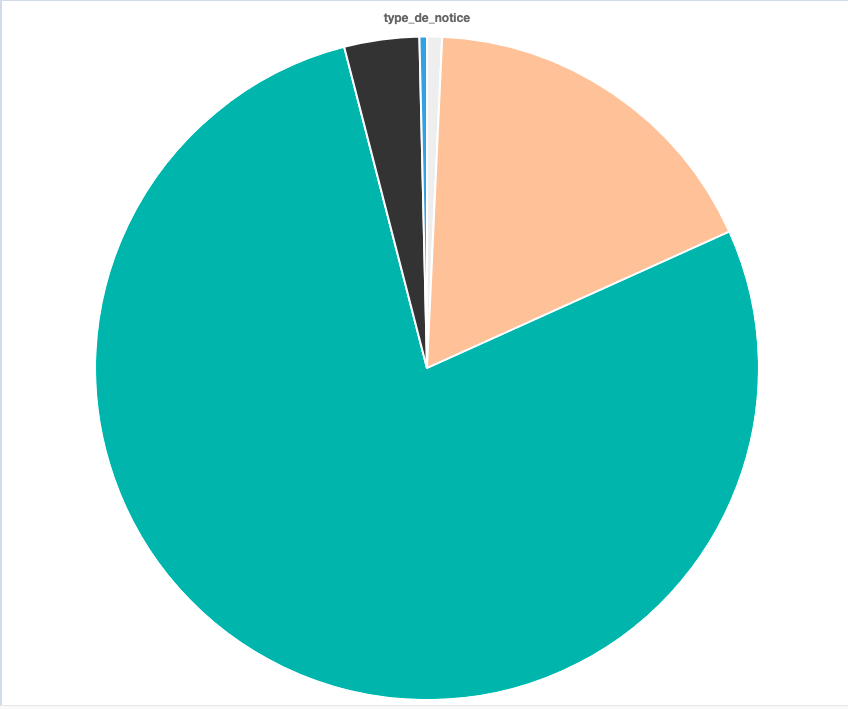
\includegraphics[width=0.5\textwidth]{Images/graphique_typo_documents.png}
    \caption{Mêmes données que sur l'image précédentes, cette fois affichées sous la forme d'un graphique sectoriel.}
    \label{fig:graphique-typologie}
\end{figure}

\clearpage 
Dans le cas présent, ce graphique contient peu de catégories, c'est pourquoi il est lisible. Toutefois, ce type de visualisation est déconseillé au-delà de six catégories car les parts sont trop petites, donc l'oeil n'arrive plus à différencier les proportions\footcite[p. 83]{lagnel_2021}. Ainsi, même si elle est simple d'utilisation et intégrée à \emph{Heurist}\index{Heurist}, cette datavisualisation n'est pas toujours intéressante et est à limiter à certains cas. Cette forme de graphique est la seule visualisation possible dans \emph{Heurist}\index{Heurist} à partir des \emph{Crosstabs}. Si l'on souhaite d'autres représentations graphiques à partir des données Heurist, il reste possible d'exporter les données et de les réutiliser dans un logiciel adapté, comme \emph{Tableau}\index{Tableau}, logiciel de référence en matière de datavisualisation. 

Toutes ces possibilités d'interrogation et de visualisation de la base servent donc à exploiter nos données de recherche. Elles peuvent également avoir pour but de préparer les données afin de les rendre accessibles à un public large\footcite[\enquote{Mettre en ligne les données gérées dans Heurist}]{paillusson_introduction_2022}. 

\section{Favoriser l'accessibilité des données et mettre en valeur le travail : un site internet conçu à partir de la base}

La base doit pouvoir être publiée et documentée. Cet impératif répond au besoin de valoriser ce projet de recherche en cours, mais aussi de garantir l'accessibilité des données, conformément, là encore, au principes de la science ouverte. C'est pourquoi nous avons utilisé la possibilité, intégrée à \emph{Heurist}\index{Heurist}, de créer un site web à partir de la base de données\footnote{Le lien vers le site web est disponible dans les annexes, dans la section \enquote{\ref{website}}.}. En effet, le mode \emph{Publish} du logiciel permet de publier les données sur le web sous la forme d'un CMS. Cet acronyme signifie \emph{Content Management System}, et désigne un programme informatique permettant de gérer l'apparence et le contenu d'un site web de manière centralisée\footcite{noauthor_content_nodate}. 

Contrairement à des sites web HTML plus classiques, les sites générés à partir d'\emph{Heurist} ne sont pas développés avec un code HTML complet\footcite[Le langage HTML (\emph{Hypertext Markup Language}), est un langage de programmation déclarative, de description de l'information]{margaux_faure_2025}, assorti d'une feuille de style CSS\footcite[Le langage CSS (\emph{Cascading Style Sheets}), permet de travailler l'apparence d'un site web en lui appliquant des règles de style]{margaux_faure_2025}. 
Une fois généré par le bouton \emph{Create} du mode \emph{Publish} et ouvert en mode \enquote{édition}, le site peut être agencé à l'aide de la fonction \emph{Website editor}. Les pages du site sont choisies parmi des formes pré-conçues prévues par \emph{Heurist}\index{Heurist}. Son contenu textuel est géré par des bouts de code HTML à placer dans des formulaires de saisie répartis à différents endroits de l'éditeur du site. L'esthétique du site (polices d'écriture, couleurs, ...) est définie par des bouts de code en CSS, également à saisir dans des formulaires. Le site créé dans le cadre de notre projet s'est inspiré de l'agencement des pages et du texte des sites générés à partir des autres bases \emph{Heurist} de la BnF. Nous avons aussi repris les bouts de code CSS de ces autres sites pour les injecter dans le nôtre, ce qui a nécessité quelques modifications pour les ajuster au contenu de notre site. Ce choix a été fait dans un souci de cohérence avec les pratiques de l'institution, afin d'inscrire notre base dans la continuité des projets similaires menés à la BnF. L'intérêt principal du site web, à savoir l'accès aux données de la base, réside dans les filtres et \emph{facets} évoqués dans la partie précédente. Ces modes d'interrogation de la base sont réutilisables dans le site web, ce qui donne un accès direct aux données par des recherches avancées et des visualisations. Chaque table de la base sur les factures Rondel est donc interrogeable dans le site sur une page dédiée. La page \enquote{lieu} donne accès à la carte des lieux indexés dans la base, et la page \enquote{personne} aux réseaux de libraires. Les pages \enquote{facture} et \enquote{ligne de facture} permettent, quant à elles, d'interroger respectivement les deux tables par de nombreux filtres de recherche. Il faut noter que le site web permet de retrouver n'importe quelle donnée de la base grâce à des barres de recherche plein texte réparties sur les différentes pages du site. 

Ce site web répond donc au besoin de publicité et d'accessibilité des données. Cependant, il comporte certaines limites et incertitudes, spécifiques aux sites web \emph{Heurist}\index{Heurist} ou plus générales. Si un site web CMS correspond aux objectifs d'Heurist, à savoir permettre une utilisation minimale de programmation pour en élargir l'accès, cela n'est valable que pour le développement d'un site web minimaliste. Si l'on souhaite personnaliser l'esthétique et la forme ou l'adapter à une forme standard, comme nous l'avons fait dans le cadre de ce projet, l'édition requiert certaines compétences en développement web. De plus, développer un site web par petits bouts de code éparpillés est très déroutant, et la documentation n'est pas suffisante pour en comprendre précisément le fonctionnement. 

\vspace{1.5cm}
Enfin, la création de ce site web a suscité quelques questions, pour l'instant restées en suspens et au stade expérimental. Nous nous sommes interrogés sur un potentiel besoin d'avoir des formes normalisées des principales informations sur les oeuvres. Cette réflexion est partie du constat que des informations importantes peuvent être lacunaires ou mal orthographiées dans les factures, ce qui rendrait le requêtage difficile. Nous avons aussi constaté que les champs issus des catalogues de la BnF ne suffiraient pas à pallier à cette difficulté, car les notices des catalogues sont parfois incomplètes et ne sont pas toujours uniformes. Ainsi a été créée une section supplémentaire dans la table \enquote{ligne de facture}, dont les champs visent à saisir des formes normalisées des titres, des auteurs, des éditeurs et des lieux. Les formes à saisir sont, elles aussi, définies dans la documentation sur les usages de la base. Tous ces champs sont donc  publiés à titre d'exemple sur le site web, mais ont été essayés sur très peu d'enregistrements pour l'instant. 
L'incertitude qui demeure au sujet de la normalisation concerne le dédoublement des informations que cela pourrait entraîner, entre les champs de normalisation et les champs dédiés aux données issues des catalogues. Les données sont censées être normalisées dans les catalogues en ligne. La meilleure solution à long terme serait donc de pouvoir s'en contenter. Que cette idée soit maintenue ou non dans les futurs usages de la base, la question de la normalisation est essentielle, et devra se poser. 



	%etc.
\section{Conclusion de la deuxième partie}

Dans cette deuxième partie, les différentes étapes de la conception de cette base de données \emph{Heurist}\index{Heurist} ont été présentées. Nous avons vu que celle-ci ne peut pas se faire sans un travail conséquent et extérieur au logiciel au préalable, partant d'une analyse minutieuse des sources dans le but de réaliser un premier modèle de données, et d'une identification des besoins et des usages de la future base de données. Ce travail préparatoire pose les jalons de la conception, cette fois avec \emph{Heurist}\index{Heurist}, de la base qui doit être prioritairement envisagée comme une transcription d'un maximum d'informations issues des factures. Enfin, nous avons pu envisager les différents besoins auxquels peut répondre cette base Heurist, de l'enrichissement des données à leur réutilisation en passant par leur publication, sans oublier les nombreuses datavisualisations envisageables, qu'elles soient nativement intégrées au logiciel ou permises par des exports. Cependant, toutes ces utilisations sont plutôt d'ordre expérimental pour l'instant, et ne peuvent pas être pérennisées sans perspectives claires d'alimentation de cette base de données. 

    \part{Perspectives envisagées pour l'implémentation et les usages ultérieurs de la base de données}

Cette troisième partie entend présenter les perspectives envisagées pour alimenter et implémenter la base. Cette réflexion finale part des constats dressés à ce stade sur les différentes façons possibles d'alimenter la base de données à partir des factures, et sur ce qui est envisageable ou non à long terme pour traiter le reste du corpus. Nous présenterons ensuite les différentes expérimentations faites en ce sens, notamment l'utilisation de l'intelligence artificielle dans le traitement de ces documents et ce qui a été mis en place au sein du département suite à ces réflexions. Nous reviendrons pour finir sur les tentatives échouées ou non abouties dans ces essais. 

\chapter{Bilan des différents modes d'implémentation de la base}

Afin d'en améliorer le modèle et d'en explorer les possibilités, la base de données a déjà été alimentée à ce stade du travail par plus de cent cinquante factures. Cela a également permis de tirer des conclusions sur les modes d'alimentation de la base en elle-même et de réfléchir aux méthodes à employer à l'avenir. 

\section{Premières réflexions sur l'utilité potentielle de l'IA pour traiter ce corpus}

À une époque où l'intelligence artificielle (IA) se perfectionne dans la reconnaissance d'écritures, notamment manuscrites, la question de son utilisation doit nécessairement être posée dans le cadre de l'exploitation d'un corpus aussi massif que le nôtre. En effet, la visée finale de cette base serait de recenser les données de l'ensemble des factures issues des archives d'Auguste Rondel. Comme nous l'avons vu, ces factures remplissent une vingtaine de boîtes d'archives. Il en existe donc au moins une dizaine de milliers. Si l'indexation de toutes les factures paraît déjà très longue en imaginant que l'on puisse utiliser une solution d'automatisation, il semble totalement hors de portée de saisir toutes les données à la main. En effet, cela nécessiterait des années de travail et une mobilisation à temps plein de plusieurs personnes, ce qui n'est pas envisageable. Nous avons donc très rapidement réfléchi aux solutions dont nous disposions pour utiliser l'IA dans la transcription des factures. 

La solution la plus efficace et privilégiée à ce stade est l'utilisation de \emph{Gemini}\index{Gemini}, assistant IA de Google. Cette utilisation, dont les modalités seront détaillées ultérieurement, consiste à récupérer un maximum d'informations des factures, puis à les structurer au format CSV afin de pouvoir les importer dans la base. Les travaux les plus concluants sont disponibles en annexe \footnote{Voir dans l'annexe E, \enquote{\nameref{prompt gemini}}.}.


\section{Estimations du temps pris par les différents modes de transcription}

Au-delà d'alimenter la base, nos expérimentations nous ont aussi permis d'estimer le temps moyen que peuvent prendre ces différentes façons d'exploiter les factures. Ces estimations confirment largement le besoin d'automatiser le traitement du corpus. Le temps pris par la saisie manuelle de factures a notamment été mesuré sur le dossier consacré à la librairie  Claudin. Ce dossier est le seul à avoir été entièrement saisi manuellement dans la base et est constitué de 16 factures, chacune composée de moins de 10 titres. Ce dossier, de petite taille et dont les factures contenaient assez peu d'informations par rapport au reste de l'échantillon, a été saisi sur une durée de trois jours environ. La saisie manuelle de certaines factures a été chronométrée. Variable selon les cas, elle va de 15 à 20 minutes pour les factures les moins fournies à environ une heure pour les plus denses. 

Nous avons ensuite estimé le temps que prenait la principale solution d'utilisation de l'IA que nous avions à disposition, à savoir \emph{Gemini}\index{Gemini}. Notre usage a surtout servi à transcrire des factures de la librairie Hermal qui, à l'inverse des factures précédente, figurent parmi les plus denses de notre échantillon. Contenant une dizaine de lignes chacune, celles-ci comportent beaucoup d'informations exploitables sur chaque titre acheté. Nos estimations réalisées sur cinq de ces factures ont montré que leur traitement automatique suivi de l'import des données nécessitait entre 4 et 6 minutes au total. 

La conclusion de ces estimations est très claire : le traitement des factures par IA, en particulier en utilisant \emph{Gemini}\index{Gemini}, est beaucoup plus rapide que la saisie manuelle. 

\section{Limites de ces estimations}

Malgré tout, il est nécessaire de rester prudent sur ces estimations. Celles-ci ont été faites à partir d'un échantillon qui, comme nous l'avons dit, n'est pas représentatif de l'ensemble des factures. Si nos conclusions sont valables à cette échelle  restreinte, une part d'incertitude demeure car le corpus est massif. Il n'est donc pas possible de tout anticiper ni de se projeter sur l'exploitation du corpus dans son ensemble, car nous n'en avons traité qu'une infime partie pour l'instant. 
\chapter{La transcription automatique, une solution privilégiée pour implémenter la base de données ?}

Dans notre utilisation de l'IA pour traiter les factures Rondel, la principale technologie expérimentée est la reconnaissance d'écritures manuscrites, ce qui semple plutôt logique au vu de la nature du corpus. S'il est essentiel de revenir sur l'histoire de cette technologie, ce chapitre vise surtout à présenter les différents tests réalisés sur les factures Rondel et ce qui a été mis en place par le département pour poursuivre le projet. 

\section{La \emph{Handwritten Text Recognition}, ou la reconnaissance automatique d'écritures manuscrites}

La grande majorité des factures traitées jusqu'à présent est de nature manuscrite. Pour les transcrire, il convient donc de s'intéresser à une technologie nommée \emph{Handwritten Text Recognition} (HTR), utilisant l'intelligence artificiele et spécialisée dans la reconnaissance et la transcription d'écritures manuscrites. Cette technologie est à distinguer de l'\emph{optical character recognition} (OCR), qui est plus ancienne\footcite[Voir][La naissance de l'OCR est souvent attribuée au physicien Emmanuel Goldberg qui, durant la Première Guerre mondiale, invente une machine permettant de lire des caractères et de les convertir en code télégraphique]{lefevre_locr_2023} et vise à transcrire des caractères imprimés\footcite[p. 1]{gutteridge_judge_2026}. La HTR est initialement fondée sur une collaboration entre l'IA et l'être humain, qui a pour rôle d'améliorer les performances de la machine par l'utilisation de corpus d'entraînement\footcite{pinche_2022}. Tout comme l'OCR, les outils traditionnels de la HTR fonctionnent en trois étapes. Cela commence par un prétraitement de documents numérisés, suivi d'une analyse et d'une segmentation de leur mise en page pour enfin en transcrire le texte\footcite[p. 1]{kim_early_2025}. 
Cependant, les évolutions actuelles dans ce domaine montrent que tous les outils de HTR connus jusqu'à présent sont aujourd'hui largement surpassés par les modèles de langage\footnote{Deux principaux types de modèle de langage sont à distinguer : les LLM (Large Language Modele), qui ne traitent que des données textuelles et les VLM (Vision Language Modele) qui, associant les technologies des LLM à des outils de vision, sont aussi capables de traiter des images.}, modèles d'IA générative permettant notamment de transcrire, de classer et de comprendre des documents\footcite[p. 1]{crosilla_benchmarking_2025}. Le type de modèle de langage ayant particulièrement fait évoluer la transcription automatique est le VLM, par sa capacité à traiter des images, ce que ne peut pas réaliser le LLM. Ces modèles n'ont pas besoin d'être entraînés et ne se contentent pas de transcrire l'écriture manuscrite. Ils sont également capables d'identifier la mise en page des documents, d'extraire, de structurer et d'analyser le sens des informations et de les exporter\footcite{sebastien_cretin_2025}. De plus, tout le travail n'est réalisé qu'en une seule étape du point de vue utilisateur\footcite[p. 1]{kim_early_2025}. Il faut surtout retenir que les capacités de ces modèles de langage s'améliorent très vite. En effet, la littérature scientifique sur le sujet affirmait encore en octobre 2024 que les performances des modèles de langage, \emph{Gemini}\index{Gemini} en particulier, étaient nettement inférieures à celles des modèles entraînés pré-existants, mais qu'elles étaient prometteuses\footcite[p. 4-6]{li_handwriting_2024}. L'outil semble s'améliorer constamment depuis, au point d'être actuellement comparable, selon certaines sources, à des performances humaines\footcite{humphries_gemini_2025}. 


Ainsi, revenir sur l'histoire et les évolutions de la HTR met en évidence le fait que les grands modèles de langage, en particulier les VLM, sont aujourd'hui une solution simple et rapide à utiliser, pouvant réaliser de nombreuses tâches et de plus en plus performante. 


\section{Les différents outils de reconnaissance automatique expérimentés pour traiter les factures Rondel} 

Quelque soit les solutions expérimentées, envisager un traitement informatique de notre corpus suppose d'identifier précisément nos besoins en matière d'automatisation. L'exploitation informatique des factures est surtout utile pour alimenter la table\enquote{ligne de facture} de la base, qui comporte le plus d'informations issues des factures et qui vise à identifier les oeuvres. Ainsi, nos attendus vis-à-vis de l'IA sont l'analyse de la mise en page des factures, afin de comprendre et de transcrire un maximum d'informations susceptibles de remplir cette table. À partir de ce travail, nous souhaitons que l'IA structure les informations dans un format permettant de les importer directement dans la base. Comme évoqué précédemment, il est préférable que les informations issues de cette transcription soient structurées au format CSV, manière la plus simple d'importer des données en masse dans \emph{Heurist}\index{Heurist}. Pour que les imports soient possibles, nous avions d'autres besoins plus précis, à savoir de corriger et d'adapter certaines données pour qu'elles puissent être insérées dans la base. L'attendu majeur est que l'IA lie chaque ligne de facture à l'identifiant \emph{Heurist}
(\emph{Heurist-ID})\footnote{Voir chapitre I, partie II, \enquote{\nameref{types donnees}}.} de l'enregistrement \enquote{facture} créé au préalable, à laquelle la ligne doit être liée. Cela permet de lier directement les lignes à leur facture lors de l'import du fichier CSV\footnote{Voir page 28 à 31 de \enquote{\nameref{documentation}}.}.


La nécessité d'un outil utilisable rapidement et en mesure de répondre simultanément à plusieurs besoins a fait des modèles de langage la technologie priorisée dans l'exploitation des factures Rondel. En effet, entraîner un modèle de HTR n'est pas le but de notre projet et était trop long pour être réalisé sur le temps de mon stage. Le principal modèle de langage utilisé pour exploiter notre corpus est Gemini\index{Gemini}. Sur la durée de mon stage, plusieurs de ses modèles ont pu être expérimentés, tels que \emph{Gemini}\index{Gemini} 3.5 Flash, sorti en mai 2026, moment où nous avons commencé à utiliser l'IA. Les derniers modèles de \emph{Gemini}\index{Gemini} sont capables de réaliser des tâches parfaitement adaptées à l'exploitation des factures Rondel, à savoir la compréhension d'images, l'extraction et la classification d'informations\footcite{noauthor_liste_nodate}.
Les possibilités de traiter les factures Rondel grâce à \emph{Gemini}\index{Gemini} ont été explorées par différents prompts, incluant progressivement des consignes de plus en plus précises répondant aux exigences de notre base. Le prompt le plus complet vise à remplir le plus de champs possibles de la table \enquote{ligne de facture}. 
Ce prompt est visible en annexe, accompagné d'un exemple de facture transcrite, et du fichier CSV extrait de cette transcription\footnote{Voir \enquote{\nameref{prompt gemini}}.}. La facture, datant du 22 juin 1920, est produite par la librairie Hermal, qui a vendu beaucoup d'oeuvres à Auguste Rondel. La plupart des tests d'IA ont été réalisés sur les factures produites par Hermal, car les descriptions des oeuvres sont très complètes, ce qui donne un bon aperçu des capacités de \emph{Gemini}\index{Gemini}. L'exemple montré en annexe illustre la finesse de l'analyse textuelle faite par \emph{Gemini}\index{Gemini}. L'outil a parfaitement transcrit toutes les informations sur chaque oeuvre et les a systématiquemet rangées dans les bonnes colonnes. \emph{Gemini}\index{Gemini} parvient même à détecter certaines subtilités. C'est le cas de la distinction entre auteur et éditeur, ce qui transparaît en particulier dans la première ligne, où seul un éditeur est mentionné. On voit aussi dans les cinquième et sixième ligne que Gemini sait faire la distinction entre la date d'édition de l'oeuvre et une date faisant partie du titre de l'oeuvre. Comme Gemini ne parvient pas à interroger le catalogue général de la BnF\footnote{Ce point sera détaillé dans le chapitre suivant.}, le prompt tente malgré tout de relier chaque oeuvre à sa sous-série d'appartenance dans la collection par un moyen détourné. Il demande à \emph{Gemini}\index{Gemini} de relier chaque oeuvre à la sous-série de la collection Rondel à laquelle elle est la plus susceptible d'appartenir, ce qu'on peut voir dans la colonne \enquote{Série/sous-série} du fichier CSV. Même s'il ne s'agit que d'hypothèses, cette méthode fonctionne plutôt bien. Après vérification, quatre des six oeuvres apparaissant dans la facture du 22 juin 1920 ont été reliées à la bonne sous-série. Cependant, comme pour tous les autres traitements demandés à \emph{Gemini}\index{Gemini}, une vérification humaine est indispensable avant le moindre import de ces données dans la base, même si l'outil est très performant. Ce prompt, qui a prouvé son efficacité dans la transcription d'une facture afin d'alimenter la table \enquote{ligne de facture}, a donc été retenu et expérimenté plusieurs fois. Des consignes supplémentaires ont également été testées et peuvent être ajoutées pour améliorer le prompt. On peut par exemple demander à \emph{Gemini}\index{Gemini} de ne pas transcrire certaines lignes, si elles ne font pas référence à des oeuvres. \emph{Gemini}\index{Gemini} est également capable de transcrire plusieurs factures à la fois, si on lui indique correctement quels identifiants \emph{Heurist} écrire sur quelles lignes, pour que les lignes soient associées aux bonnes factures une fois dans la base. Il faut donc remplacer l'instruction liée à la colonne \enquote{H-ID facture} comme dans l'exemple suivant : 

\begin{quote}
    Dans la colonne "H-ID facture", ajoute 1718  sur toutes les lignes pour les factures datant du 12 novembre 1919, 1719 sur toutes les lignes pour celles datant du 4 novembre et 1720  sur celles datant du 13 octobre. 
\end{quote}

Ainsi, \emph{Gemini}\index{Gemini} est de loin l'outil le plus performant, rapide et simple d'utilisation essayé pour transcrire les factures Rondel. Malgré cela, nous nous sommes aussi intéressés aux alternatives \emph{Open Source} existantes pour réaliser ces mêmes tâches. Le principal outil expérimenté est \emph{NuExtract3}\index{NuExtract3}, publié le 19 mai 2026 par \emph{NuMind}. Il s'agit d'un modèle VLM spécialisé dans l'extraction de documents. Il réunit l'extraction structurée et la reconnaissance de caractères\footcite{numind_nuextract_nodate}. Cet outil a été testé via \emph{Hugging Face}\index{Hugging Face}, plateforme dédiée au partage de jeux de données, d'applications et modèles d'apprentissage par intelligence artificielle\footcite{noauthor_nuextract_nodate}. Cette plateforme permet une prise en main relativement simple : il suffit d'entrer le document que l'on souhaite transcrire dans la catégorie \emph{input}, de saisir au format JSON la structure des informations que l'on souhaite extraire dans \emph{Schema \& Instructions} et de cliquer sur \emph{Extract JSON}. Nous avons testé cet outil sur des factures produites par différents libraires, mais les tests les plus convaincants sont ceux réalisés sur celles de la librairie florentine \emph{de Marinis}, ou sur celles de la librairie de l'Ancien temps, située à Paris. Cela s'explique par le peu d'informations contenues dans ces factures et le fait qu'elles se présentent souvent sous forme tabulaire, avec une délimitation claire entre les différents types d'informations. Même s'il reste quelques fautes à corriger avant d'importer dans la base, l'outil est plutôt efficace. Un exemple de test réalisé sur une facture, contenant la facture elle-même, le schéma JSON utilisé pour extraire et le résultat est disponible en annexe\footnote{Voir dans l'annexe E, I.2 : \enquote{\nameref{nuextract3}}.}. Le résultat de l'extraction est structuré sous la forme d'un schéma JSON, constitué de clés (les noms des champs de la table) et de valeurs (les valeurs de ces champs pour chaque enregistrement). L'import des données JSON directement dans la base \emph{Heurist} est possible, mais cela était difficile à réaliser correctement. L'alternative choisie pour avoir des données prêtes à être importées dans la base a donc consisté en un script Python permettant de convertir le schéma JSON en un fichier CSV, lui aussi détaillé en annexe. Malgré tout, \emph{NuExtract3}\index{NuExtract3} n'a été efficace que sur certaines factures parfaitement structurées et pas trop denses. Sur d'autres factures, les transcriptions faites par cet outil étaient beaucoup moins précises, contenaient des erreurs et étaient mal structurées. Cet outil n'est mentionné ici que parce qu'il est plus performant que les autres outils \emph{Open Source} testés sur les factures Rondel. Malgré tout, sa pertinence reste nettement inférieure à celle de \emph{Gemini}\index{Gemini}, car il est plus lent, transcrit moins bien et n'est pas conçu pour réaliser automatiquement tous les traitements nécessaires.  

Toute transcription automatique des factures est suivie d'un import, de préférence au format CSV, dans la base. Pour que l'import soit réussi, il est très important de sélectionner le bon séparateur, caractère permettant de diviser le texte entre les différentes colonnes, ainsi que le bon encodage, qui assure que tous les caractères soient correctement lus par le logiciel. Une fonction de prévisualisation du futur import, appelée \emph{Analyse data}, permet de s'assurer que le fichier s'importera correctement dans le logiciel. Comme évoqué au début de cette partie, les étapes de cet import sont détaillées dans la documentation sur les usages ultérieurs de la base\footnote{Voir page 28 à 31 de \enquote{\nameref{documentation}}}. 


Tous ces essais d'utilisation de l'IA dans le traitement des factures Rondel ont permis de dresser un constat principal. Celui-ci est, nous l'avons vu, que \emph{Gemini}\index{Gemini} surpasse de loin tous les autres outils essayés dans le cadre de ce projet, dans toutes les phases du traitement des données. Or, il convient de rester critique envers cet outil, car celui-ci présente certaines limites qui n'ont rien à voir avec ses performances. Premièrement, \emph{Gemini}\index{Gemini} est très consommateur en énergie. Même s'il n'existe pas de données chiffrées publiques concernant cette consommation, les estimations placent \emph{Gemini}\index{Gemini} comme l'un des outils les plus consommateurs au monde. Le site ComparIA, géré par le gouvernement français et permettant de comparer les IA conversationnelles, a classé la taille du modèle en \emph{XL}\footcite{noauthor_classement_nodate}. La taille d'un modèle d'IA influe nécessairement sur sa consommation énergétique : plus un modèle est lourd, plus il consomme. De plus, \emph{Gemini}\index{Gemini} n'est pas une solution \emph{Open Source} et Google en est complètement propriétaire, ce qui explique notamment le manque de transparence au sujet de sa consommation. Il faut donc avoir conscience, lorsqu'on utilise \emph{Gemini}\index{Gemini}, que toutes les données traitées sont transmises à Google. Les modèles \emph{Open Source}, quant à eux, n'engendrent pas de fuites de données et consomment beaucoup moins que \emph{Gemini}\index{Gemini}. Par exemple, la taille de \emph{NuExtract3}\index{NuExtract3} est estimée à quatre milliards de paramètres\footcite{numind_nuextract_nodate}.
En revanche, ils sont nettement moins performants sur le plan technique, comme nous l'avons vu. 

Nos expérimentations elles-mêmes ont aussi des limites à prendre en compte. Même s'il est très important, le traitement par IA de notre corpus n'est pas l'objet principal de ce projet, ce qui explique l'absence de statistiques sur l'efficacité des différents outils essayés. Cela aurait nécessité un travail dit de \enquote{vérité terrain}, passant par la sélection d'un échantillon représentatif du corpus, et la comparaison de sa transcription manuelle et de sa transcription automatique. Nous avons simplement réalisé une preuve de concept, c'est-à-dire une démonstration visant à prouver la faisabilité d'une idée\footcite{definition_PoC}. En somme, nos analyse sont qualitatives, et non quantitatives. 



\section{La numérisation : une étape nécessaire dans le traitement des factures par intelligence artificielle} 

Un potentiel traitement massif de ces factures de libraires par IA nécessite de mettre en place leur numérisation. Au début de ce projet, aucune facture du corpus n'était numérisée. La plupart des tests d'IA ont donc été réalisés sur des photographies de factures, ce qui ne peut pas être une solution à long terme. Nous avons demandé et obtenu la possibilité de numériser les 2000 premières factures du corpus, c'est-à-dire les cinq premières boîtes. Avant d'être numérisées, les factures de chaque dossier ont été classées par ordre chronologique  lorsqu'elles ne l'étaient pas déjà, pour qu'elles apparaissent dans cet ordre sur Gallica\index{Gallica}. 
Quelques consignes supplémentaires ont été données. Par exemple, nous avons choisi de ne pas numériser les mandats de paiement, ni les documents autres que des factures contenus dans les dossiers (accusés de réception, avis de débit, ...). Ont évidemment été exclus de cette numérisation les dossiers consacrés à d'autres commerces que des librairies, qui ne seraient d'aucune utilité au remplissage de la base (ateliers de relieurs, imprimeries, ...). Ces 2000 factures de libraires sont dans Gallica\index{Gallica} et sont facilement accessibles depuis le catalogue BnF Archives et manuscrits\index{Bnf Archives et manuscrits}. Un exemple de dossier numérisé est disponible en annexe\footnote{Voir annexe E, II. \enquote{\nameref{numerisation}}.}. Ce travail de numérisation a pour objectif d'être poursuivi sur le reste du corpus dans le cadre d'une continuation de ce projet. Malgré le caractère expérimental de l'usage de l'IA dans l'exploitation des factures Rondel, cette première numérisation ouvre la voie, par les solutions actuelles ou futures, à la pérennisation de ces procédés. 



\vspace{1,5cm}
En somme, les tentatives d'utilisation de l'IA pour exploiter les factures Rondel se sont d'abord appuyées sur un état de l'art, afin d'être en phase avec les pratiques dans ce domaine. Celles-ci ont permis d'évaluer quels sont les outils adaptés aux traitements dont on a besoin, et les contraintes liées aux différents modèles. Cependant, nos essais sont limités pour l'instant et demandent à être déployés à une échelle plus large. 
\chapter{Tentatives échouées, perfectibles ou inachevées dans l'alimentation de la base}

Les réflexions sur les différents moyens d'alimenter la base de données ont surtout fonctionné par tâtonnements. Il était donc inévitable que ce travail mène aussi à des échecs ou à des idées qui, faute de temps, n'ont pas abouti. 

\section{Les limites de l'IA dans le traitement des factures}

Si les tests réalisés avec l'IA ont donné des résultats très satisfaisants, ils ont aussi mis en évidence les limites techniques des différents outils, même les plus performants. 

\vspace{1,5cm}
\emph{Gemini}\index{Gemini} reste limité sur certains aspects, c'est pourquoi il n'est pas en mesure d'effectuer à lui seul tous les traitements nécessaires à l'import des données dans la base. Comme nous l'avons évoqué dans le chapitre précédent, \emph{Gemini}\index{Gemini} n'est pas capable d'interroger les catalogues de la BnF. Dans l'espoir de lui faire remplir l'intégralité des champs de la table \enquote{ligne de facture}, nous lui avons demandé de relier les oeuvres présentes dans les factures aux notices correspondantes dans les catalogues de la BnF. L'objectif était que \emph{Gemini}\index{Gemini} remplisse la section \enquote{informations catalogue}, en renseignant les ARK des auteurs et des exemplaires, ainsi que leurs cotes dans des colonnes prévues à cet effet. À cette demande, l'outil tente de réaliser cette tâche et nous indique qu'il l'a faite, mais les résultats sont toujours très fantaisistes. Les cotes ne sont jamais les bonnes et les ARK ne renvoient à aucune page existante. On voit bien que \emph{Gemini}\index{Gemini} est capable de manipuler les informations qui lui sont données, mais ne sait pas en utiliser d'autres. 

Les limites de \emph{Gemini}\index{Gemini} ont aussi été constatées sur des traitements de données en masse. La possibilité d'accéder aux numérisations a permis d'envisager des traitements de données plus massifs, toujours pour alimenter la base. Dans les traitements précédents, il était toujours nécessaire, comme nous l'avons évoqué, de saisir manuellement un enregistrement \enquote{facture} pour pouvoir produire un identifiant \emph{Heurist} permettant de lier la facture à toutes les lignes qui la composent. Nous nous sommes donc demandés s'il était possible d'automatiser aussi la transcription des données pour remplir la table facture, puis de lier par l'intermédiaire de \emph{Gemini} les identifiants \emph{Heurist} des factures aux lignes de factures correspondantes. Cela servirait à automatiser le traitement successif de deux tables essentielles de notre base. Pour ce faire, nous avons tenté de procéder en deux prompts.
Le premier a consisté à demander à \emph{Gemini}\index{Gemini} de transcrire et structurer toutes les informations utiles au remplissage de la table \enquote{facture}. Pour cela, un fichier PDF de factures numérisées a été joint au prompt suivant :

\begin{quote}
    Voici un ensemble de factures numérisées et produites par le même libraire  

En ne prenant en compte que les factures (donc pas les relevés ni les correspondances), peux-tu en extraire certaines informations sous forme de tableur ? 

Structure l'informations dans les colonnes suivantes : date de la facture, prix total, frais, commentaire facture, dossier, librairie H-ID (laisser la colonne vide)

Dans la colonne "dossier", mettre la valeur suivante : RCOL-1(<À COMPLÉTER EN FONCTION DU DOSSIER>)
\end{quote}

Ce prompt a fonctionné. Malgré quelques corrections à effectuer, le fichier CSV produit contenait les informations demandées sur les trente-trois factures numérisées du libraire Georges Chrétien et a pu être importé dans la base. Nous avons donc fourni à \emph{Gemini}\index{Gemini} l'instruction servant à remplir \enquote{ligne de facture}. En plus du dossier numérisé, nous avons joint à ce prompt un export CSV, issu de la base, des dates et des identifiants \emph{Heurist} des trente-trois enregistrements \enquote{facture} correspondants. Le prompt contenait une instruction supplémentaire demandant à \emph{Gemini}\index{Gemini} d'analyser les dates des factures et de les lier aux identifiants \emph{Heurist}\index{Gemini} issus de l'export CSV correspondant à ces dates. \emph{Gemini}Gemini\index{Gemini} n'a pas du tout pu réaliser cette tâche, répondant simplement qu'il n'était qu'un modèle de langage et que cette demande dépassait ses compétences. Le test a ensuite été simplifié : le fichier CSV contenant les identifiants \emph{Heurist} a été retiré des pièces jointes, et les instructions qui allaient avec ont été supprimées. Cela visait à voir si Gemini parvenait à remplir la table \enquote{ligne de facture} à partir d'un dossier entier numérisé. Cette fois, \emph{Gemini}\index{Gemini} a tenté de réaliser la tâche, mais le résultat n'était pas satisfaisant, car toutes les lignes n'ont pas été transcrites et dans les rares cas où elles l'ont été, il y avait beaucoup trop d'erreurs. 

Plusieurs outils expérimentés n'ont pas donné de résultats convaincants. Tous nos tests sont détaillés dans une documentation spécifique, dont le lien est accessible dans les annexes\footnote{Voir \enquote{\nameref{doc IA}}}. Nous avons par exemple essayé l'outil \emph{Corpusense}\index{Corpusense}, fonctionnant sur l'utilisation de \emph{Mistral AI}\index{Mistral AI}, autre modèle de langage\footnote{\emph{Corpusense} a été expérimenté avec l'aide de Joseph Chazalon, enseignant-chercheur au laboratoire de recherche de l'EPITA et de Jonathan Perrinet, ingénieur dans ce même laboratoire.}. Nous ne nous sommes pas attardés sur cet outil, qui n'est pas idéal pour traiter les factures Rondel, mais il a produit certains résultats intéressants, comme indiqué dans la documentation. 

\section{Idées non retenues}

Dans l'espoir de faciliter l'exploitation du corpus par une solution \emph{Open Source}, une solution pour améliorer l'utilisation de l'outil \emph{NuExtract3} présenté précédemment a aussi été envisagée. Cette suggestion a été faite par Fantin Le Ber, chargé de projet de recherche au département des Arts du spectacle dans le cadre du projet TORNE-H, visant à intégrer l'intelligence artificielle dans les processus de traitement documentaire et scientifique des collections muséales\footcite{noauthor_torne-h_nodate}. Cette solution consistait à créer une application intégrant les traitements réalisés par \emph{NuExtract3}\index{NuExtract3}, grâce à Streamlit\index{Streamlit}, un outil \emph{Open Source} permettant de développer des applications grâce à \emph{Python}\footcite{noauthor_streamlit_nodate}. L'application envisagée prévoyait d'entrer une facture, de la traiter par \emph{NuExtract3} et d'en extraire directement un fichier CSV prêt à être importé dans la base. Cependant, du fait du manque de temps et des résultats peu prometteurs de cette solution d'IA par rapport à ceux de \index{Gemini}\index{Gemini} sur les factures Rondel, cette idée a rapidement été écartée. 

Il faut surtout retenir de ce dernier chapitre qu'il s'intéresse à la réflexion autour de ce qui a échoué ou n'a pas abouti dans ce travail. Ces tentatives sont essentielles à prendre en compte pour comprendre tout le reste de notre raisonnement, mais aussi pour avoir des pistes d'améliorations en vue d'une suite de ce projet. En effet, vu la vitesse à laquelle progresse l'IA dans la transcription et la structuration de données, ce qui n'est pas possible techniquement à ce stade le sera peut-être ultérieurement. 

\section{Conclusion de la troisième partie}

En somme, cette troisième partie a fait le point sur les différents modes d'alimentation de la base de données que nous avons testés à ce stade et nous a permis d'envisager différentes pistes pour ses futurs usages. 


	\chapter*{Conclusion générale}

Ce mémoire détaille le projet, porté par le département des Arts du spectacle de la Bibliothèque nationale de France, d'exploiter les archives relatives à la bibliothèque d'Auguste Rondel. Notre propos se focalise sur le traitement des factures émises par les libraires où Auguste Rondel se fournissait pour constituer sa collection, dans l'objectif de concevoir une base de données grâce au logiciel \emph{Heurist}\index{Heurist}. 


La première partie entend contextualiser le besoin de modéliser une base de données sur les factures de la collection Auguste Rondel, ce qui suppose d'abord de saisir la place occupée par la collection dans la constitution du département des Arts du spectacle. Celle-ci est à la base de la création du département, qui s'est construit autour d'elle et vise à en assurer la continuité. Avant de présenter la modélisation de la base de données, il convient de revenir sur la composition du corpus exploité, à savoir les factures Rondel, afin de comprendre à quels besoins celui-ci est susceptible de répondre. Cette présentation du corpus nous amène à confirmer qu'une base de données relationnelles est une solution adéquate pour l'exploiter, pour sa capacité à lier de nombreuses données entre elles et à les traiter. Le logiciel \emph{Heurist}\index{Heurist}, servant à la création de bases de données relationnelles, est l'outil privilégié dans notre projet. Ce choix s'explique par son accessibilité sans compétences avancées en programmation, soit à un public relativement large et par sa capacité à répondre aux enjeux propres aux projets de recherche en sciences humaines et sociales. Tous les choix évoqués s'inscrivent nécessairement dans la continuité de pratiques professionnelles et scientifiques, s'appuyant sur un état de l'art pré-existant. Ainsi sont évoquées les différentes bases de données qui existent à la BnF, conçues ou non avec \emph{Heurist}\index{Heurist}. 


La deuxième partie s'attache à détailler les différentes étapes de la conception de la base de données, de sa modélisation à son implémentation avec Heurist. Elle commence par revenir sur le travail effectué en amont, à savoir une analyse très précise des sources en vue d'en dégager des thématiques principales servant de socle à la future base. La conception d'une base de données est d'abord intellectuelle et extérieure à tout logiciel, ce qui explique la réalisation d'un modèle de données avant d'utiliser \emph{Heurist}\index{Heurist}. Ce travail s'est accompagné d'hypothèses sur les usages de cette base et les besoins auxquels elle pourrait répondre, même s'il est nécessaire de ne pas trop les anticiper, afin de ne pas restreindre la portée de la base. Tout cela amène à présenter la conception de la base de données avec \emph{Heurist}\index{Heurist}, envisagée en premier lieu comme une extraction stricte des informations issues des factures, puis comme une possibilité d'enrichir ces données, de les réutiliser ou de les visualiser. 


La troisième partie sert surtout à dresser un bilan des différentes tentatives d'implémentation de la base de données faites pour l'instant, dans le but d'envisager des perspectives pour ses futurs usages. À partir des estimations effectuées, notre réflexion constate une obligation d'utiliser l'intelligence artificielle pour transcrire les factures, car la taille du corpus rend la saisie manuelle inenvisageable. En partant de l'histoire de la transcription automatique, nous avons pu expérimenter différents outils représentatifs de ce qui existe actuellement dans ce domaine. Ainsi, le chapitre 8 relate en particulier nos essais réalisés avec \emph{Gemini}\index{Gemini}, modèle de langage le plus efficace actuellement dans la transcription, la compréhension et la structuration de données manuscrites. Nous résumons également les tests faits avec \emph{NuExtract3}\index{NuExtract3}, solution \emph{Open Source} d'une efficacité moindre, mais capable malgré tout de réaliser certaines tâches. La conclusion ressortant de tous ces tests est que les futures utilisations de cette base sont soumises à un choix principal. Celui-ci oppose des modèles de langage surpassant largement toutes les autres solutions, mais en consommant énormément d'énergie et en ne protégeant pas du tout les données utilisées, à des solutions Open Source nettement inférieures dans leur capacité, mais moins énergivores et sans fuites de données. Cette partie finit par mentionner les tentatives ratées ou non abouties dans ce travail, dont la prise en compte est essentielle pour comprendre le projet dans son ensemble, mais aussi pour retenir ces idées et les perfectionner en vue d'une continuation de ce projet. 

\vspace{1,5cm}
Les utilisations futures de cette base de données posent plusieurs questions sur une éventuelle suite de ce projet au sein du département. Tout d'abord, il est légitime de réfléchir aux moyens concrets de poursuivre ce travail, au-delà de tous les aspects très expérimentaux que nous avons évoqués jusqu'à présent. Comme il n'est pas possible de faire travailler les équipes du département des Arts du spectacle à plein temps sur ce projet, l'alimentation de la base pourrait faire l'objet de prestations ou de stages qui y seraient entièrement consacrés. Tous les usages de la base sont entièrement documentés, ce qui invite à poursuivre le travail. Cependant, rien n'empêche de faire des modifications ou des améliorations. Au contraire, celles-ci sont bienvenues si elles permettent de gagner en efficacité. Comme il serait très long d'exploiter le corpus dans son intégralité, on peut aussi se demander si ce projet parviendra à s'installer à long terme au sein du département et malgré des éventuels changements d'équipe. En somme, les pistes explorées pour l'instant offrent surtout un aperçu de ce qui est réalisable et invitent à un déploiement à plus large échelle du traitement des factures Rondel.
	\addcontentsline{toc}{chapter}{Conclusion}
\newpage{\pagestyle{empty}\cleardoublepage}
	






%%%%%%%%%%%%%%%%%%

\appendix %Des appendices: tables figures, etc

\chapter{Modélisation de la base de données \enquote{Factures de la collection Auguste Rondel}}
\clearpage
\section{Modèle de données}

\begin{figure}[htbp] \fbox{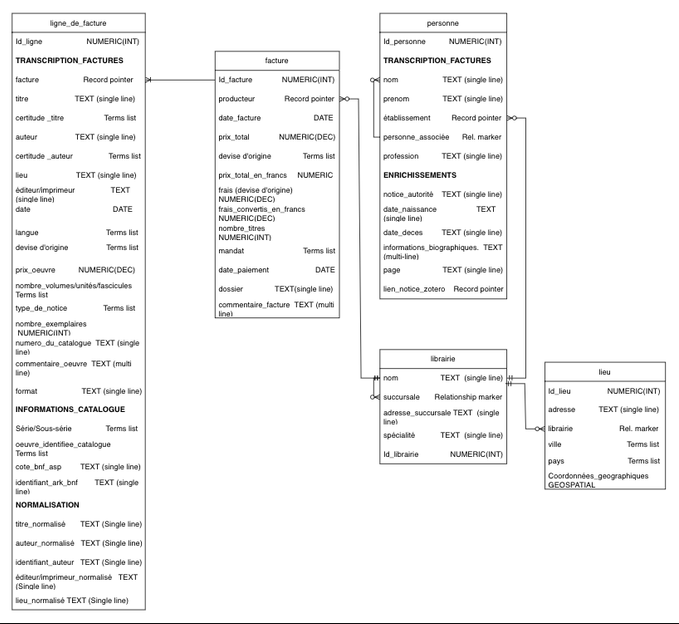
\includegraphics[width=1.0\textwidth]{Images/MLD_derniere_version.png}}
    \caption{Modèle de données réalisé avec \emph{draw.io}\index{draw.io}.}
    \label{fig:mld-drawio}
\end{figure}
\label{modele donnees}

\newpage
Il est possible de visualiser ce modèle de données de manière plus précise sur le logiciel \emph{draw.io}\index{draw.io} en cliquant sur le lien suivant : \url{https://app.diagrams.net/#G1rub2hNmAUDRaU_mgHjMSNRP601i0o7sH#%7B%22pageId%22%3A%22nmYLSE-Rn7Mf-2gKj097%22%7D}

\section{\emph{Minimum Viable Product} (MVP)}

Un tableau a été réalisé pour hiérarchiser les priorités en amont de la création de la base de données. Celui-ci est également visible sur \emph{draw.io}\index{draw.io} en cliquant sur le lien suivant : \url{https://app.diagrams.net/#G19YEhMSevG4visk5QzzYGG7j6c19q3Q0G#%7B%22pageId%22%3A%22vw2RHDlUk2C9YS3ShuU5%22%7D}
\label{MVP}

\chapter{Base de données \emph{Heurist}\index{Heurist} : \enquote{Factures de la collection Auguste Rondel}}

La base de données \enquote{Factures de la collection Auguste Rondel} a été créée avec l'instance du logiciel \emph{Heurist} hebergée par \emph{Huma-num} et est accessible en cliquant sur le lien suivant :

\vspace{1,5cm}
\url{https://heurist.huma-num.fr/heurist/?db=BnF_ASP_Rondel&w=a&q=sortby%3A-m}

Il est possible de se connecter grâce aux identifiants suivants : 

Username : raphael\_hache

Password : Gabriel22:) 

\chapter{Documentation produite pour les usages ultérieurs de la base}
\section{Livrable de recommandations - usages ultérieurs de la base Heurist\index{Heurist} sur les factures Rondel}
\label{documentation}

Cette annexe est un document d'une trentaine de pages, répondant à une demande de mes encadrantes et destiné aux futurs utilisateurs de cette base. Elle dresse d'abord une typologie des factures rencontrées dans l'échantillon utilisé, puis détaille les différentes façons d'exploiter les factures et d'alimenter la base (transcription automatique, saisie manuelle, ...). L'objectif est de documenter le projet, mais aussi d'envisager sa continuation en donnant des recommandations. 

Le document est accessible par le lien suivant : 
\url{https://github.com/Raphhache/HACHE_annexes_memoire_M2/blob/main/HACHE_Raphael_Recommandations_usages_base-2.pdf}

\pagebreak
\section{Documentation et recommandations sur l'usage de l'IA dans l'exploitation des factures}
\label{doc IA}
Cette documentation rend compte des tous les tests de transcription automatique réalisés dans le cadre de mon stage. Il s'agit d'un bilan, mais aussi de recommandations pour qui souhaite expérimenter tous ces outils sur ce corpus ou sur d'autres. Le lien suivant permet de la consulter : 

\url{https://github.com/Raphhache/HACHE_annexes_memoire_M2/blob/main/transcription%20automatique%20des%20factures%20-%20tests%2C%20prompts%20et%20recommandations.pdf}

\chapter{Datavisualisations}

\clearpage
\section{Réseaux}
\subsection{Réseaux réalisés avec \emph{Heurist}\index{Heurist}}
\label{reseaux heurist}

\begin{figure}[htbp]
    \centering
 \fbox{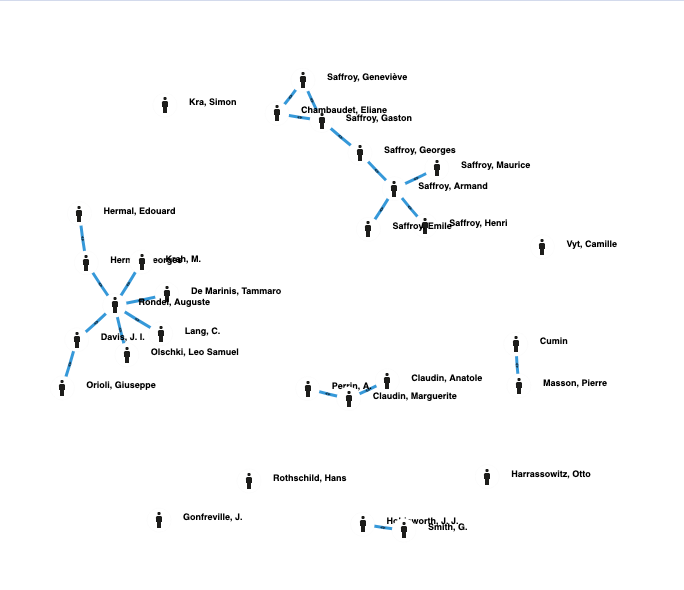
\includegraphics[width=1.0\textwidth]{Images/reseau_table_personnes_net.png}} % Nouvelle commande utilisée : la commande "fbox", qui permet de mettre des contours autour d'une image. Je l'ai beaucoup utilisée dans mes annexes car de nombreuses images étaient faites sur fond blanc. 
    \caption{Réseau visible dans la base \emph{Heurist}\index{Heurist} représentant l'ensemble des relations modélisées dans la table \enquote{personne}.}
    \label{fig:reseau-personnes-heurist}
\end{figure}

\begin{figure}[htbp]
    \centering
   \fbox{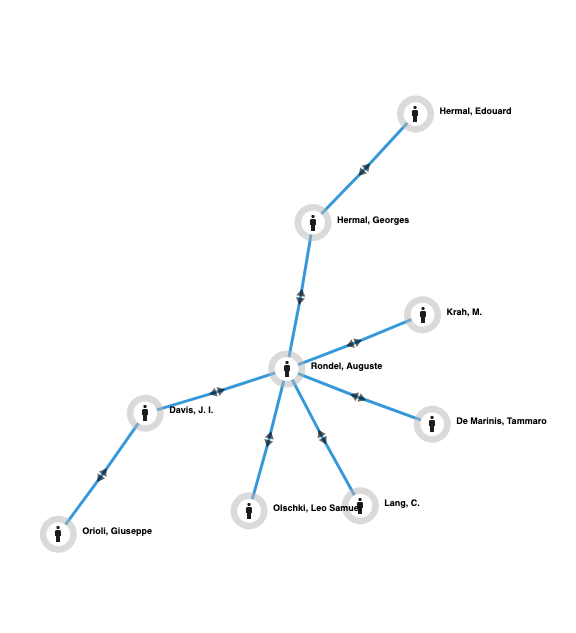
\includegraphics[width=0.8\textwidth]{Images/reseau_corresp_Rondel.png}}
    \caption{Zoom sur le réseau constitué autour d'Auguste Rondel, relié à tous les libraires avec lesquels il a entretenu une correpondance.}
    \label{fig:reseau-rondel}
\end{figure}

\begin{figure}[htbp]
    \centering
   \fbox{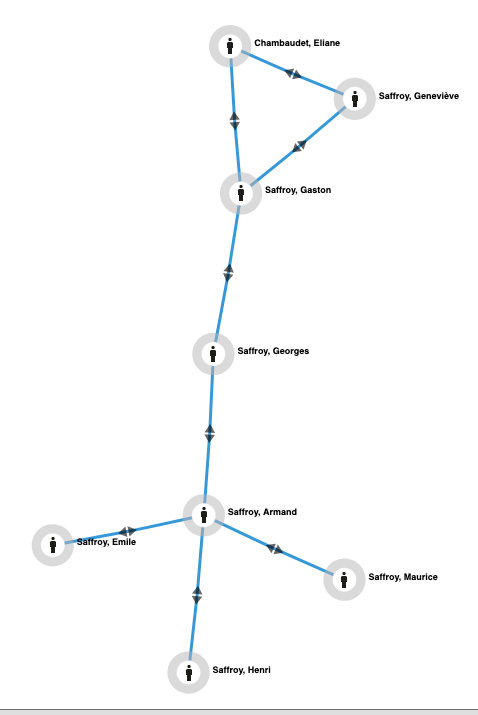
\includegraphics[width=0.8\textwidth]{Images/reseau_saffroy.png}}
    \caption{Zoom sur le réseau modélisant la famille Saffroy, qui a fait l'objet d'une recherche approfondie dans le cadre de notre travail (Voir p. 57).}
    \label{fig:reseau-saffroy}
\end{figure}


\newpage
\subsection{Exemple d'export d'un réseau de la base avec \emph{gephi}\index{Gephi} : la table \enquote{personne}}
\label{reseau gephi}
\begin{figure}[htbp]
    \centering
 \fbox{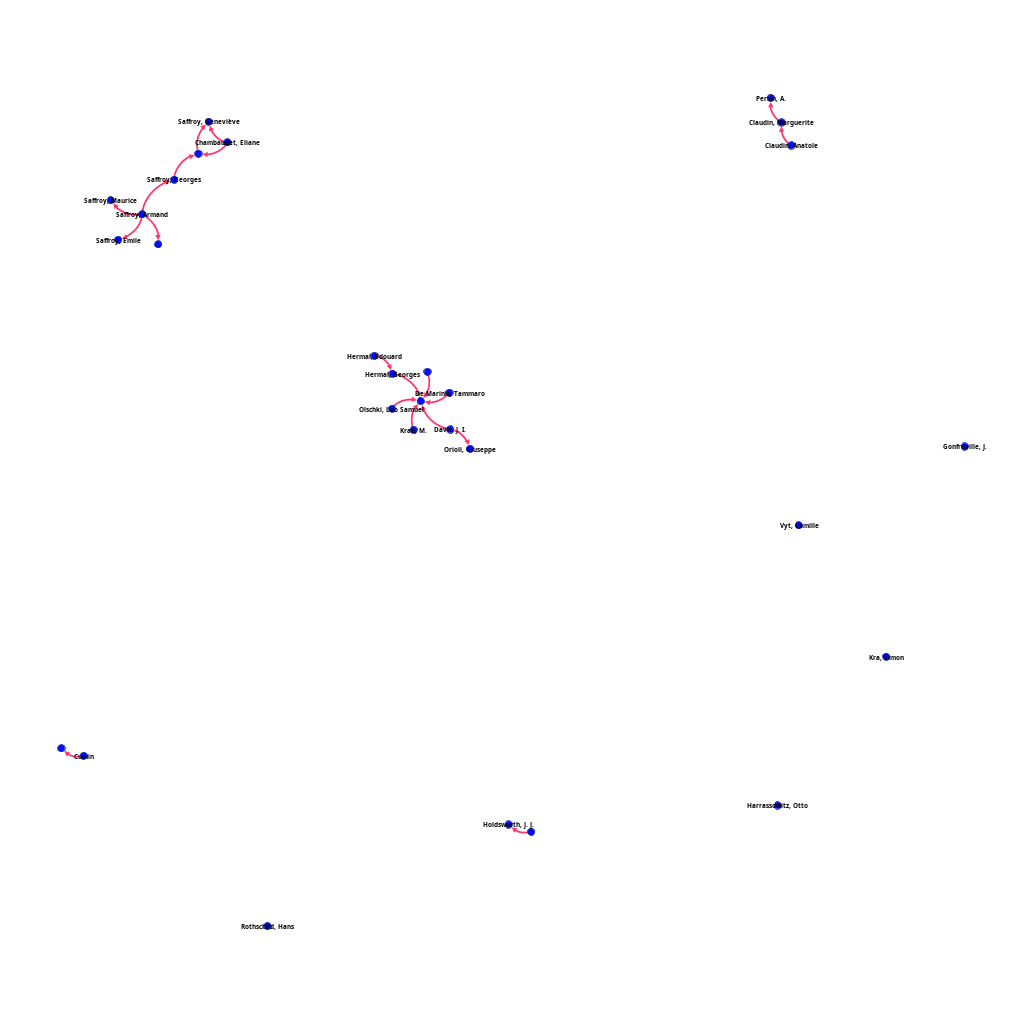
\includegraphics[width=0.8\textwidth]{Images/personnes.png}}
    \caption{Export de toutes les relations de la table personne en format .gexf dans le but de visualiser le réseau et de le mettre en forme sur le logiciel \emph{gephi}\index{Gephi}. Les noeuds (= personnes) sont représentés en bleu, et les liens (= relation) en rouge.}
    \label{fig:reseau-gephi}
\end{figure}

\newpage

\section{Cartes}
\subsection{Cartes réalisées avec \emph{Heurist}\index{Heurist}}
\label{cartes heurist}


\begin{figure}[htbp]
    \centering
 \fbox{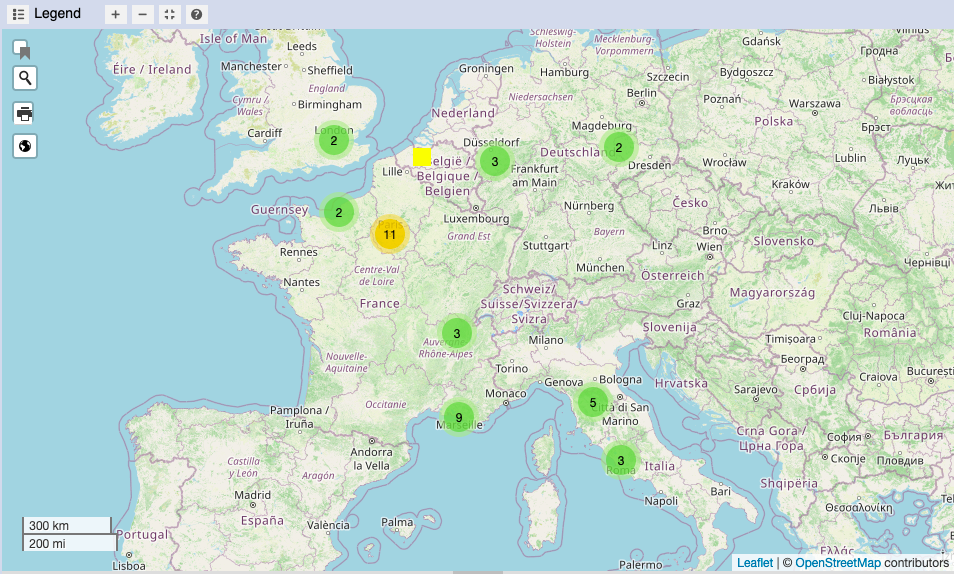
\includegraphics[width=0.9\textwidth]{Images/Carte_adresses_base.png}}
    \caption{Carte de toutes les librairies géoréférencées dans la base, grâce au champ \enquote{coordonnées geographiques} de la table \enquote{lieu}.}
    \label{fig:carte-adresses}
\end{figure}

\begin{figure}[htbp]
    \centering
 \fbox{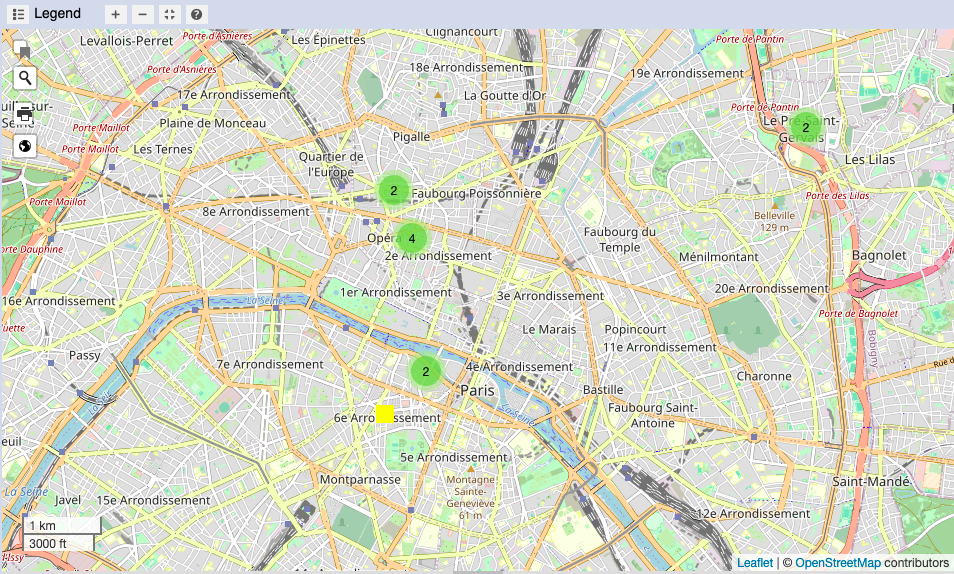
\includegraphics[width=0.9\textwidth]{Images/zoom_Paris.png}}
    \caption{Zoom sur les librairies parisiennes.}
    \label{fig:librairies-paris}
\end{figure}


\clearpage
\subsection{\emph{QGIS}}
\label{carte qgis}
\vspace{1,5cm}
\begin{figure}[htbp]
    \centering
 \fbox{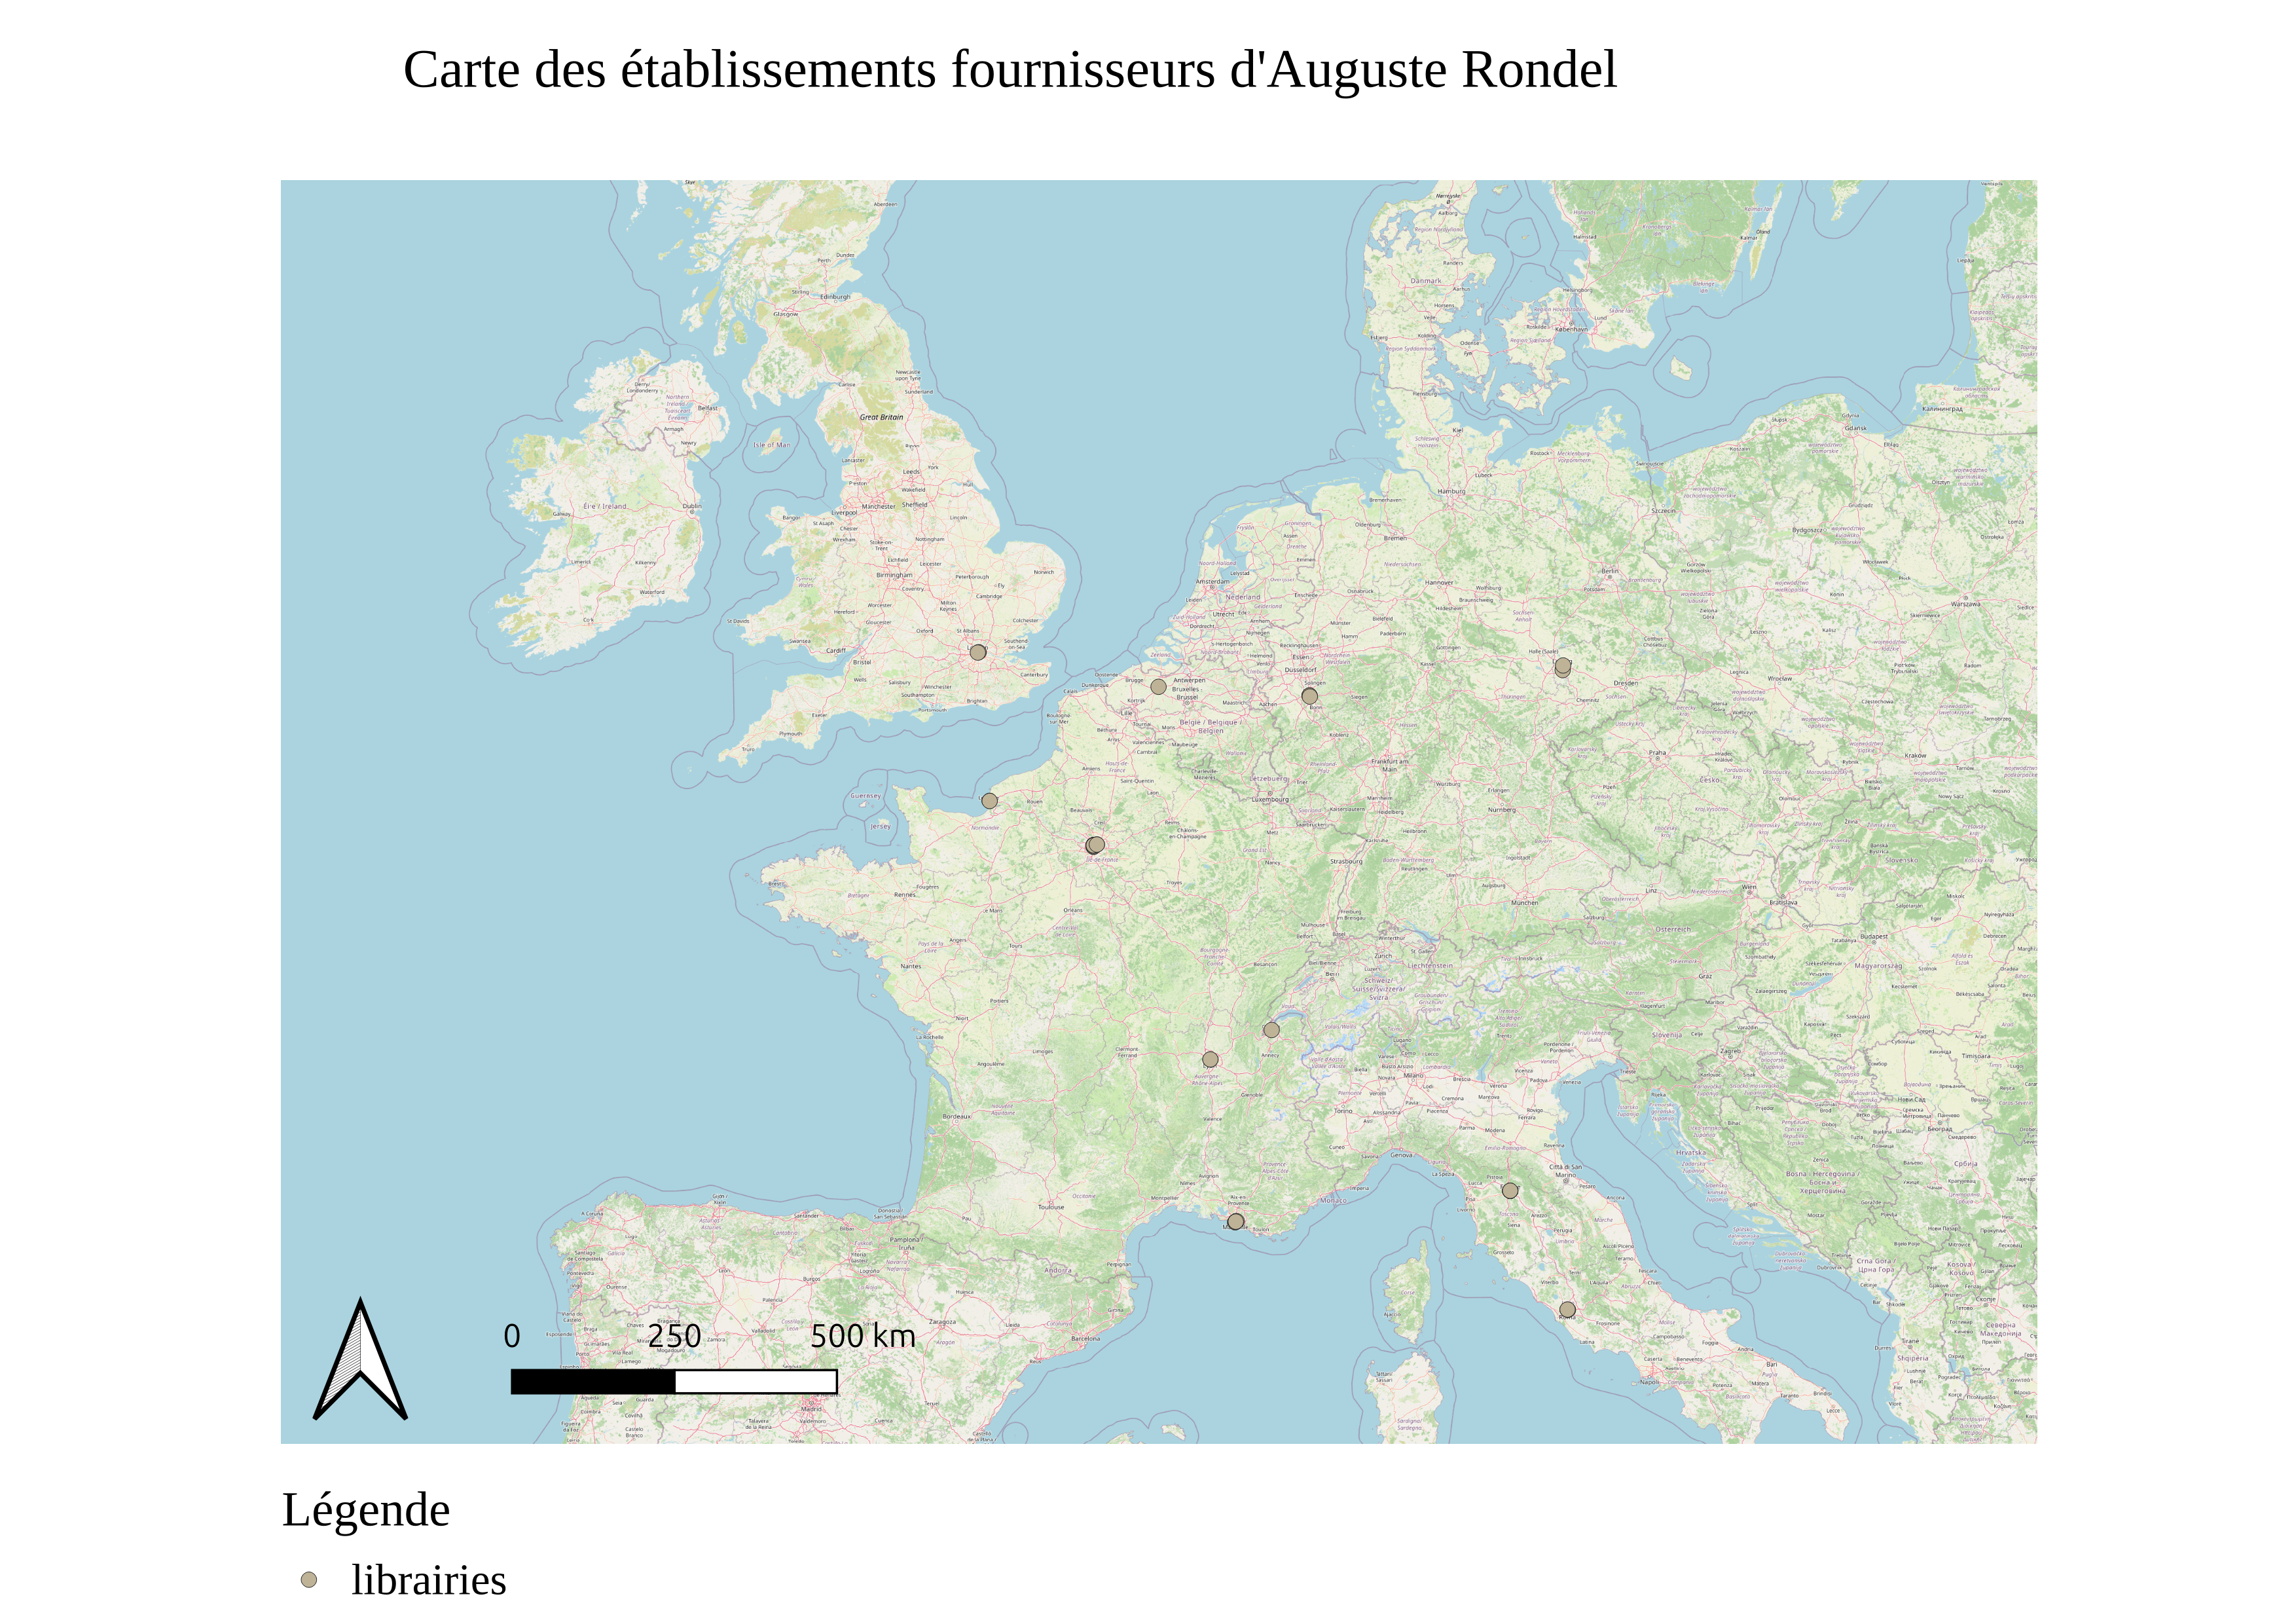
\includegraphics[width=16cm]{Images/carte_libraires_europe_v2.png}}
    \caption{Carte réalisée avec le logiciel \emph{QGIS}\index{QGIS} grâce à l'export des données cartographiques de la table \enquote{lieu} en format .geojson.}
    \label{fig:carte-qgis-europe}
\end{figure}
\newpage
\subsection{Plateforme Galligeo\index{Galligeo}}
\label{carte galligeo}


\begin{figure}[htbp]
    \centering
 \fbox{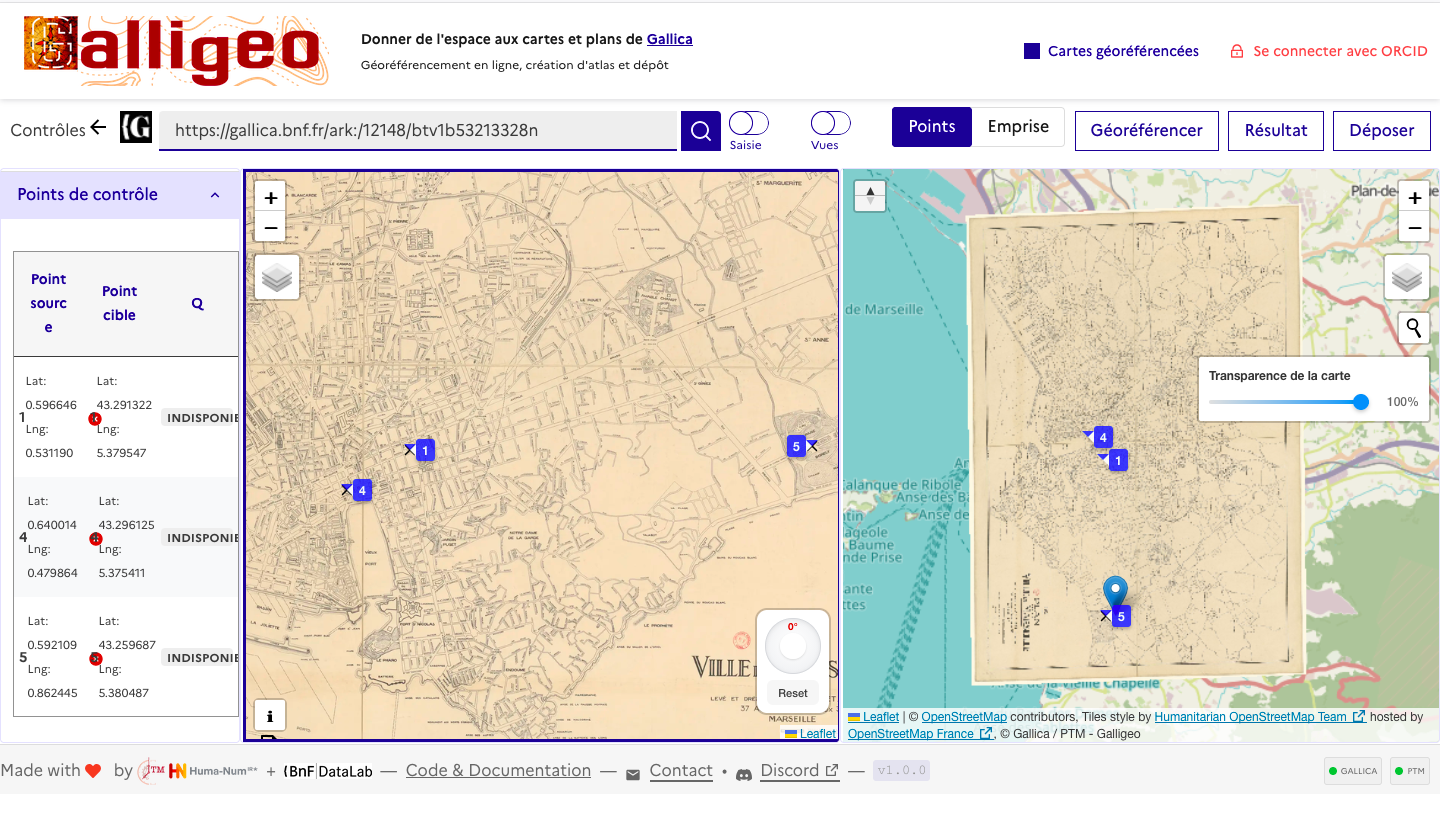
\includegraphics[width=15cm]{Images/georef_pt_ctrle.png}}
    \caption{Géoréférencement par points de contrôle sur Galligeo\index{Galligeo}.}
    \label{fig:georeferencement-galligeo}
\end{figure}

\begin{figure}[htbp]
    \centering
 \fbox{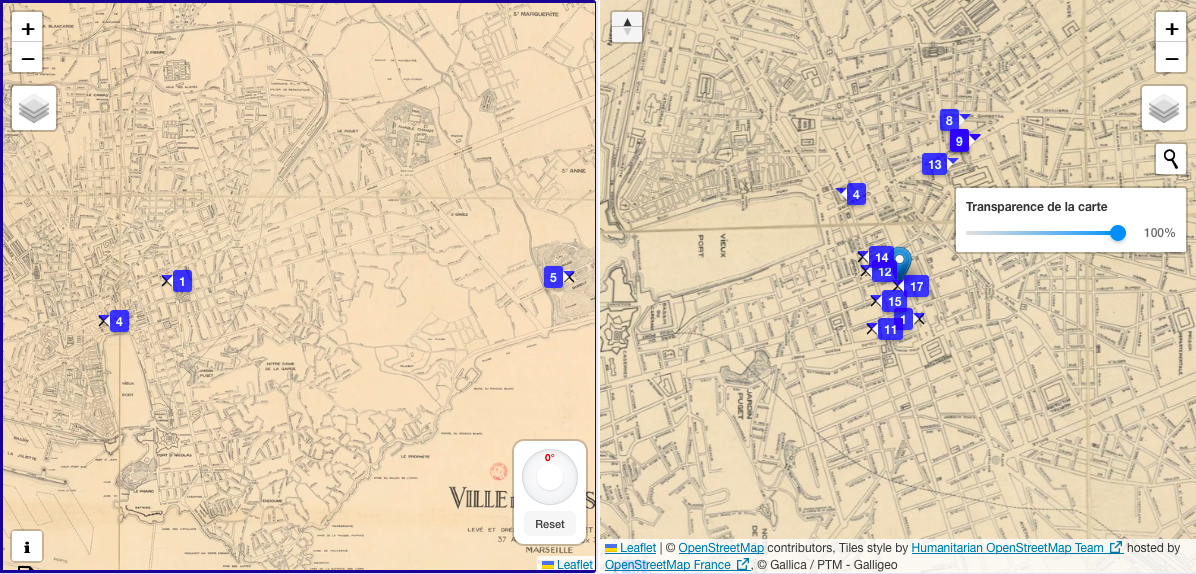
\includegraphics[width=15cm]{Images/indexation_librairies_marseille.png}}
    \caption{Indexation de toutes les librairies marseillaises où Auguste Rondel s'est fourni, sur un fonds de carte datant de 1931.}
    \label{fig:librairies-marseille}
\end{figure}

La carte ayant servi à tester cet outil est accessible en cliquant sur le lien suivant : 
\url{https://gallica.bnf.fr/ark:/12148/btv1b53213328n}

\clearpage
\section{Site web développé à partir de la base de donées}
\label{website}

\vspace{1,5cm}
Le site internet CMS développé à partir de la base de données est accessible en cliquant sur le lien suivant : 

\url{https://heurist.huma-num.fr/heurist?db=BnF_ASP_Rondel&website=1823&pageid=1841}
\vspace{1,5cm}
\begin{figure}[htbp]
    \centering
 \fbox{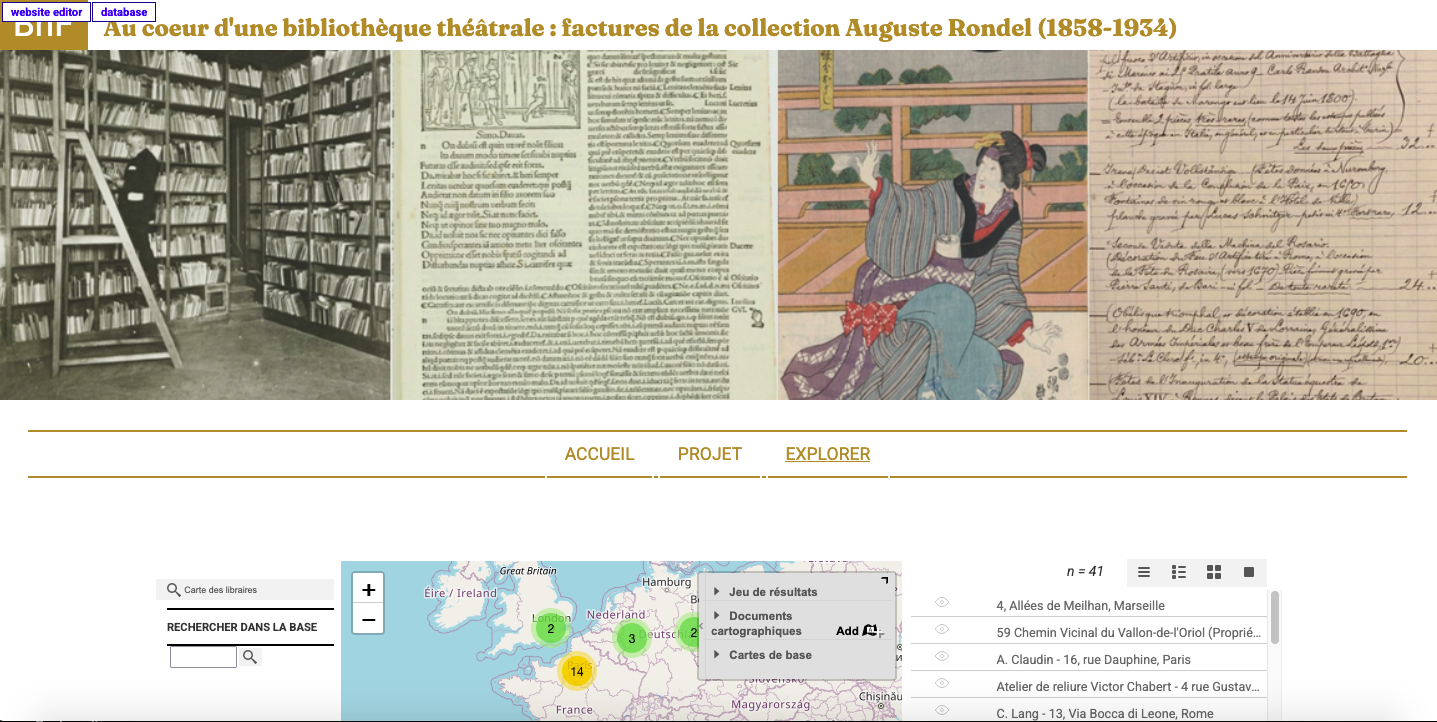
\includegraphics[width=0.8\textwidth]{Images/page site web.png}}
    \caption{Page \enquote{lieu} du site web.}
    \label{fig:site-web-lieu}
\end{figure}



\newpage

\chapter{Utilisations de l'intelligence artificielle dans le traitement des factures Rondel}
\section{Tests : exploitation du corpus à l'aide de l'intelligence artificelle}

\subsection{Tests réalisés avec \emph{Gemini}\index{Gemini}}
\label{prompt gemini}

\vspace{1,5cm}
\underline{Prompt :}
\vspace{1,5cm}

Voici une page de facture, peux-tu en extraire les informations sous forme de fichier csv ? 

structure l'information dans les colonnes suivantes : titre, auteur, lieu, éditeur, date, devise d'origine, prix oeuvre, nombre volumes/unités/fascicules, nombre exemplaires, numéro du catalogue, langue, format, commentaire oeuvre, H-ID facture, Série/sous-série

mets uniquement des nombres entiers pour le nombre de volumes et le nombre d'exemplaire 

écris simplement le nom de la devise, sans abréviation 

mets la devise au singulier et sans majuscule 

Dans la colonne "H-ID facture", ajoute  <l'identifiant Heurist correspondant à la facture> sur toutes les lignes 

fais en sorte que les dates respectent le format date, ou mets "circa" quand c'est une date approximative  

Écris dans "type de notice" à quelle catégorie l'oeuvre appartient parmi les suivantes : 


archives
dessin
estampe
monographie
périodique
photographie
reliure




Identifie les thématiques de chaque oeuvre et classe les parmi les intervalles de cotes suivants : 


RA (Fêtes)
RA1-87 (Pyrotechnie)
RA2 1-125 (Châteaux)
RA3 1-387 (Spectacles de cour en France)
RA4 1-1788 (Fêtes et entrées françaises)
RA5 1-1574 (Fêtes et entrées italiennes)
RA6-RA17 (Fêtes et spectacles de cour : Allemagne, Autriche, Angleterre, Espagne, Belgique, ...)


RAE (Estampes : fêtes, spectacles de cour)
RE (Théâtre étranger)
RE 1-1314 (Théâtre grec)
RE 11200-11999 (Théâtre américain)
RE 12000-15349 (Théâtre allemand)
RE 1315-1934 (Théâtre latin)
RE 15371-15752 (Théâtre hollandais)
RE 15756-15807 (Théâtre flamand)
RE 15816-17131 (Théâtre belge)
RE 17151-17917 (Théâtre d'Europe centrale et des Balkans)
RE 17918-18592 (Théâtre russe)
RE 18593-18599 (Théâtre ukrainien)
RE 18610-19579 (Théâtre scandinave)
RE 1935-2458 (Théâtre oriental)
RE 19581-20126 (Théâtre suisse)
RE 2459-6055 (Théâtre italien)
RE 6056-7199 (Théâtre espagnol)
RE 6961-7024 (Théâtre portugais)
RE 7125-7182 (Théâtre latino-américain)
RE 7200-11199 (Théatre anglais)
RE 10993-11063 (Théâtre irlandais)
RE 7578-8838 (Théâtre élizabethain)
RE 7893-8788 (Shakespeare)
RF (Théâtre français)
RF 1-962 (Théâtre français - Moyen Age)
RF 15200-19899 (Théâtre français - XVIIIè siècle - Révolution)
RF 1578-7390 (Théâtre français - XVIIè siècle)
RF 19900-36993 (Théâtre français - XIXè siècle : 1800-1850)
RF 36994-49478 (Théâtre français - XIXè siècle : 1850-1890)
RF 49501-75078 (Théâtre français - XXè siècle : 1890-1936)
RF 7391-11135 (Théâtre français - XVIIIè siècle)
RF 75101-75688 (Théâtre des Jésuites)
RF 75701-76368 (Fêtes de province)
RF 76369-81107 (Théâtre des provinces et des colonies)
RF 81108-81978 (Théâtre de plein air)
RF 82311-82608 (Théâtre aux armées)
RF 82610-84553 (Théâtre de société)
RF 84554-86924 (Théâtre pour la jeunesse)
RF 87010-87242 (Noëls)
RF 87250-87516 (Théâtre de la passion)
RF 87520-87935 (Jeanne d'Arc)
RF 87940-88093 (Napoléon)
RF 963-1577 (Théâtre français - XVIè siècle)
RJ (périodiques, mémoires, histoires littéraires)
RJ 1-540 (Périodiques français)
RJ 1300-3039 (Histoire littéraire : genres)
RJ 3040-3491 (Cercles, sociétés littéraires, presse)
RJ 3600-4401 (Critique dramatique
RJ 4402-4839 (Genres dramatiques)
RJ 550-625 (Périodiques étrangers)
RJ 760-1277 (Mémoires et biographies)
RK (Cinéma)
RK 1358-15395 (Liste alphabétique de films et suppléments)
RK 15396-16531 (Sources littéraires et adaptations de films)
RK 16600-19614 (Acteurs de cinéma)
RK 19620-19973 (Périodiques français et étrangers)
RK1-1357 (Généralités sur le cinéma, matériel publicitaire de films, production)
RO (Musique)
RO 1-586 (Généralités sur la musique)
RO 13101-13372 (Carnaval)
RO 13383-13853 (Marionnettes, Guignol, Ombres)
RO 13860-16444 (Chanson, Music-hall, Cabaret)
RO 1559-2182 (Commedia dell'arte, Théâtre de la foire, Opéra-comique)
RO 16445-16461 (Revues de music-hall)
RO 16480-17586 (Cirque)
RO 17590-17857 (Sports, Tauromachie, divers)
RO 17900-19151 (Revues)
RO 2267-4488 (Compositeurs français)
RO 4490-5975 (Art lyrique français)
RO 587-1558 (Opéra)
RO 6000-7662 (Musique allemande)
RO 6713-7400 (Wagner)
RO 7670-9673 (Musique des autres pays)
RO 9700-13100 (Danse)
RT (Histoire du théâtre)
RT 1-1405 (Histoire du théâtre)
RT 11451-13266 (Architecture)
RT 1406-1704 (Histoire des théâtres)
RT 4781-11418 (Acteurs)

Écris l'intervalle auquel l'œuvre appartient dans la colonne "Série-sous-série". 

\begin{figure}[htbp]
    \centering
 \fbox{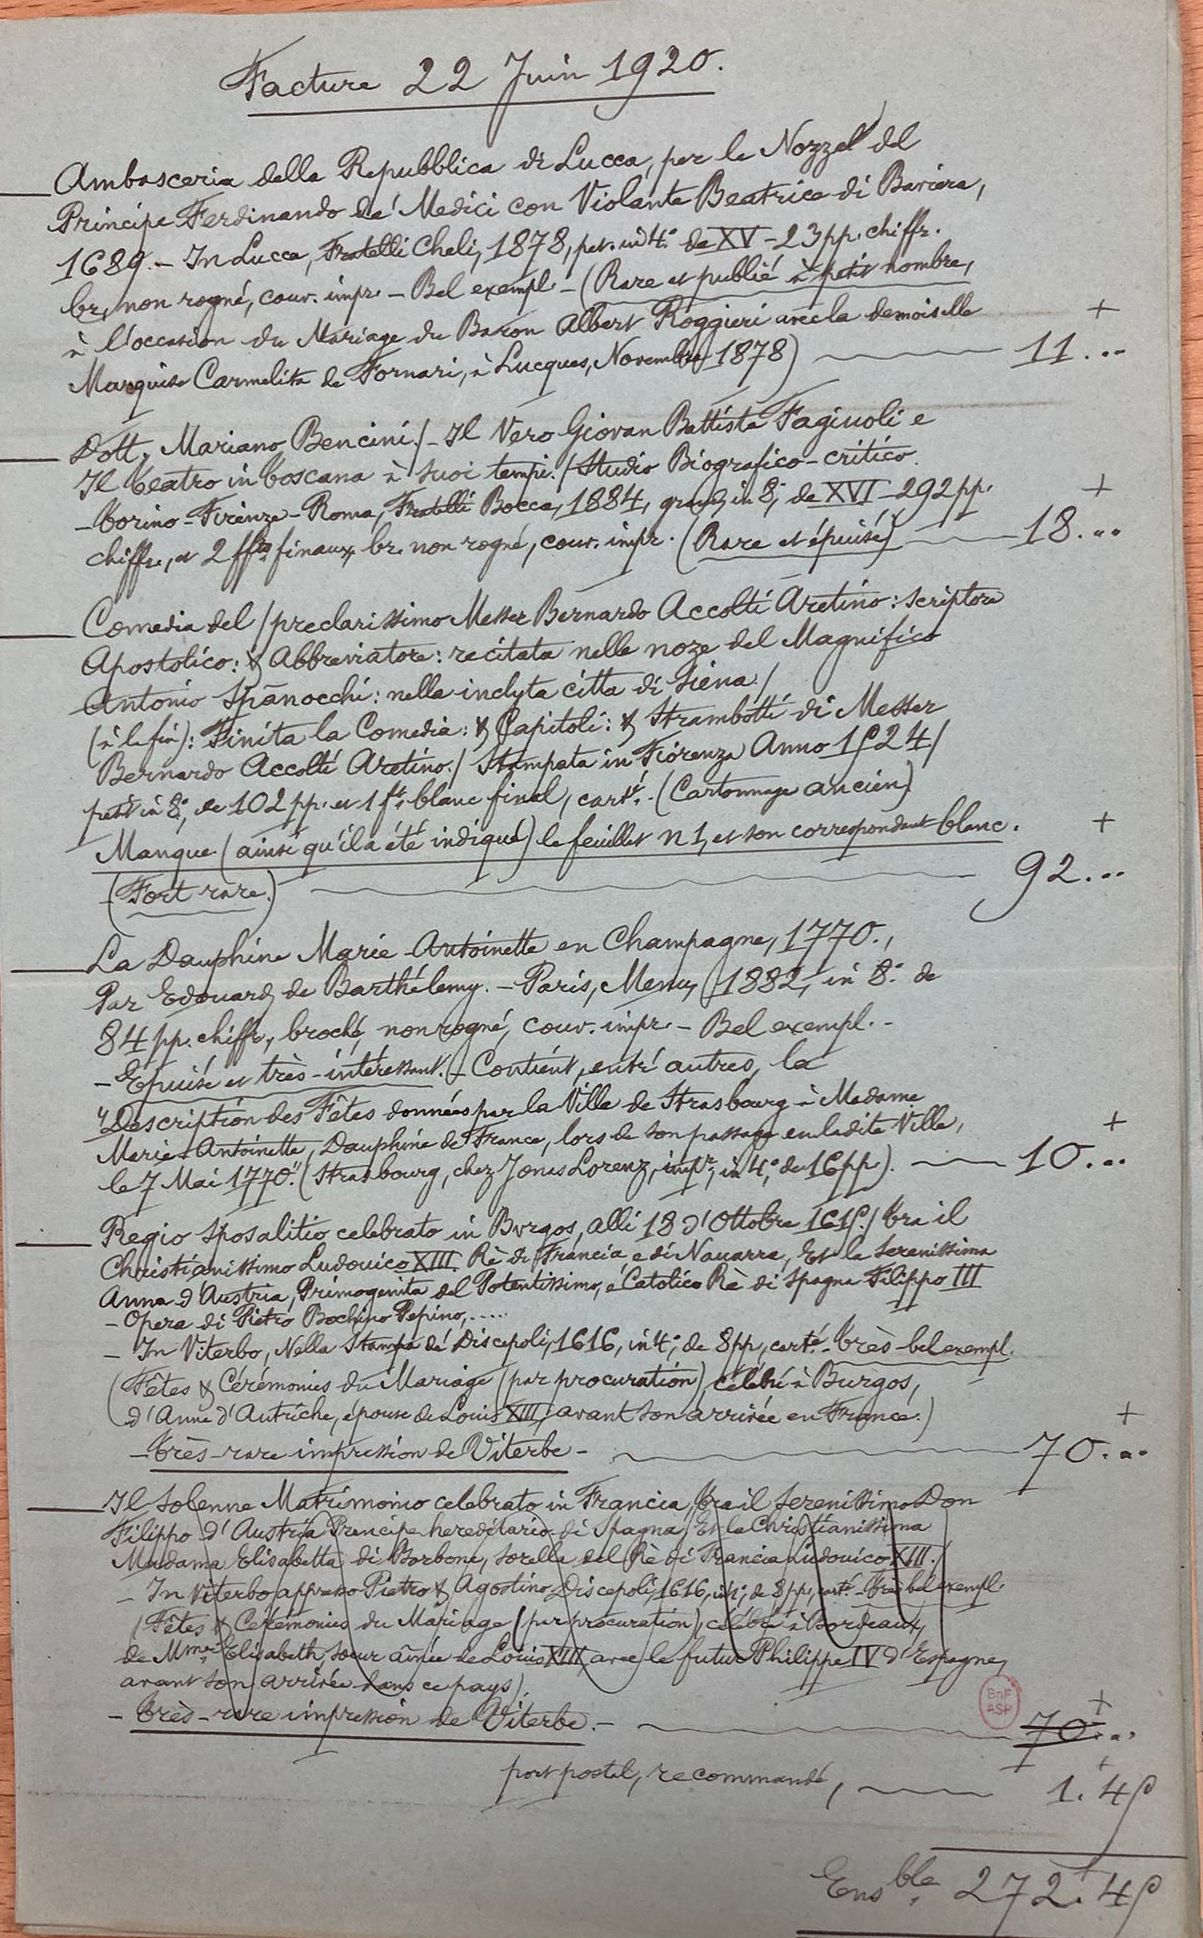
\includegraphics[width=0.7\textwidth]{Images/Hermal_8.jpeg}}
    \caption{Facture produite par le libraire Hermal, testée avec ce prompt ((BnF ASP, RCOL-1(220)). La facture est à mettre en pièce jointe du prompt.}
    \label{fig:facture-hermal-prompt}
\end{figure}

\newpage 
\underline{Fichier CSV réalisé par \emph{Gemini}\index{Gemini} à partir de cette facture :}
\vspace{1,5cm}

\url{https://github.com/Raphhache/HACHE_annexes_memoire_M2/blob/main/facture_10_juin_1920_test.csv}

\begin{figure}[htbp]
    \centering
 \fbox{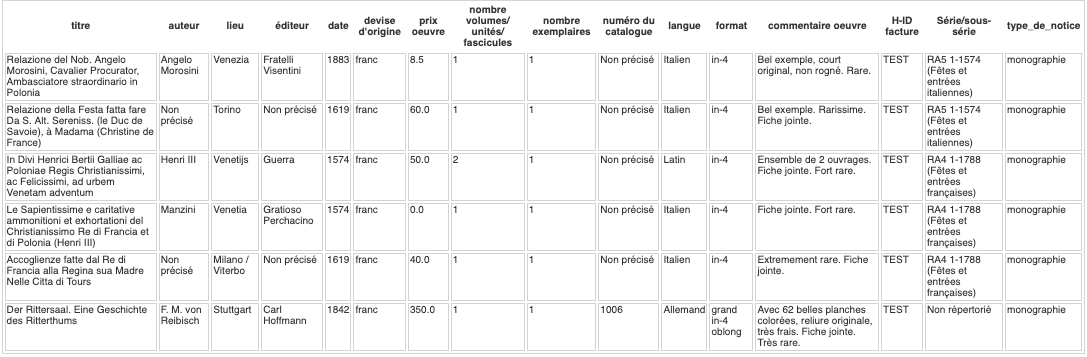
\includegraphics[width=0.9\textwidth]{Images/csv transcription gemini.png}}
    \caption{Visualisation du fichier CSV depuis \emph{Heurist}\index{Heurist}.}
    \label{fig:csv-gemini}
\end{figure}

\clearpage 
\subsection{Test réalisé avec une solution d'IA \emph{Open Source} : \emph{NuExtract3}\index{NuExtract3}}
\label{nuextract3}

\begin{figure}[htbp]
    \centering
 \fbox{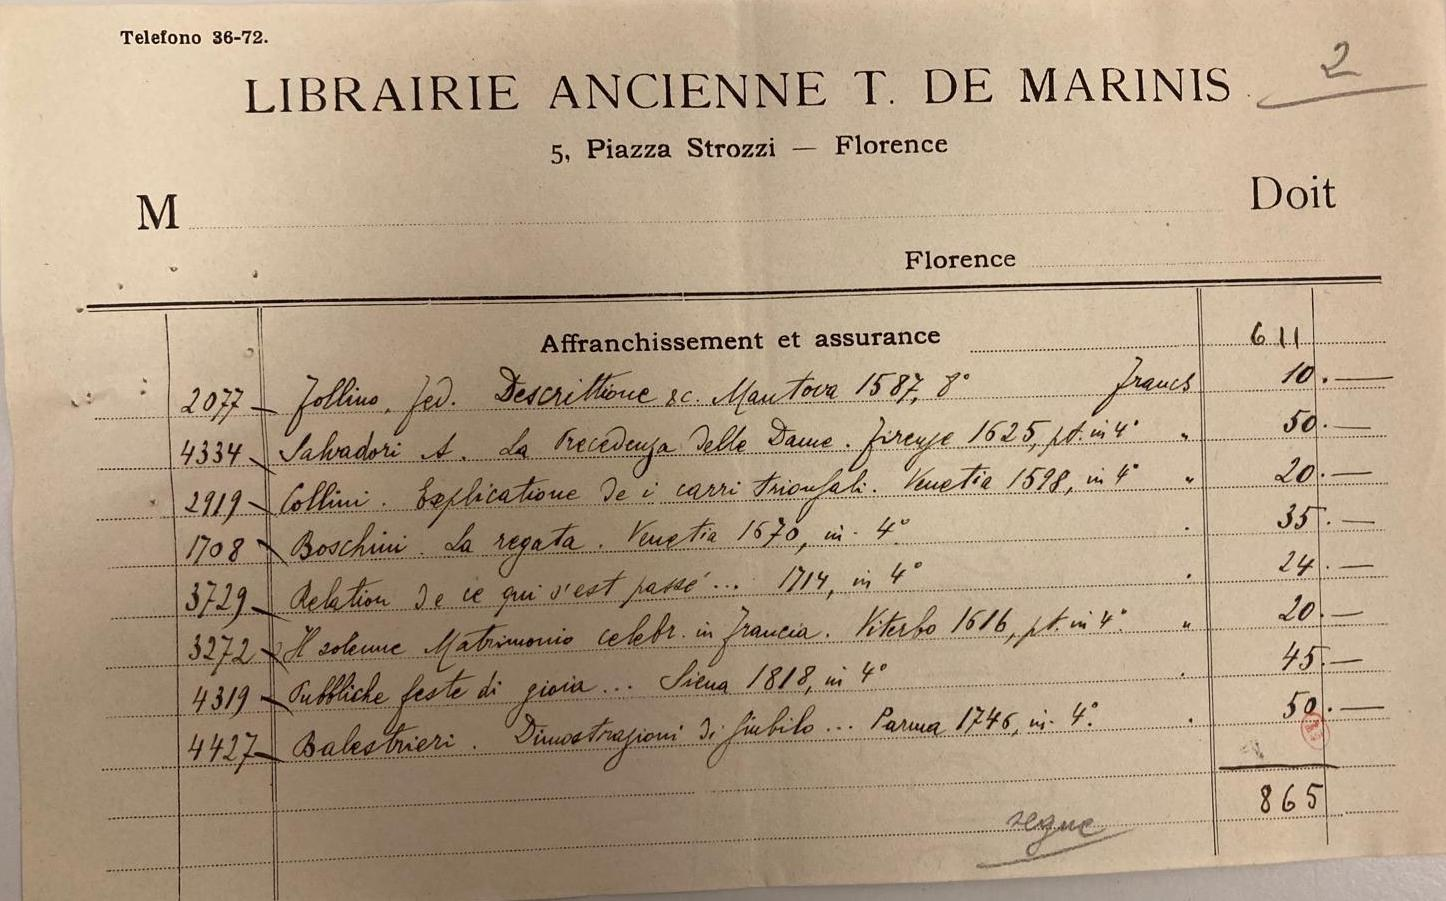
\includegraphics[width=0.9\textwidth]{Images/Marinis_2.jpeg}}
    \caption{Facture issue d'un ensemble de factures produites le 2 mai 1919 par la librairie de Marinis située à Florence. Ce document a été utilisé pour tester \emph{NuExtract3}\index{NuExtract3}.}
    \label{fig:facture-marinis}
\end{figure}

\begin{figure}[htbp]
    \centering
    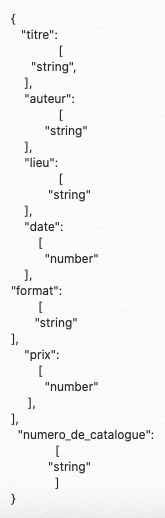
\includegraphics[width=4cm]{Images/json_entree.png}
    \caption{Schéma JSON fourni en entrée pour indiquer la structuration des données que l'on souhaite.}
    \label{fig:schema-json-entree}
\end{figure}

\begin{figure}[htbp]
    \centering
    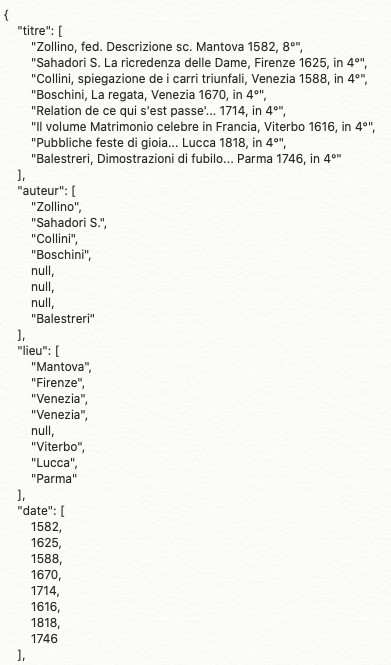
\includegraphics[width=8cm]{Images/json_sortie_1.png}
    \caption{Transcription automatique de la facture ci-dessus réalisée par \emph{NuExtract3}\index{NuExtract3}.}
\end{figure}

\begin{figure}[htbp]
    \centering
    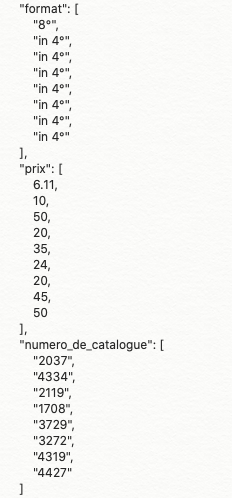
\includegraphics[width=6cm]{Images/json_sortie_2.png}
    \caption{Suite de la transcription.}
    \label{fig:json-sortie-suite}
\end{figure}

\clearpage 
\underline{Script Python :}

Le script Python sert à convertir la transcription en un fichier 
prêt à être importé dans la base. Il a été réalisé via \emph{Google Colab}\index{Google Colab}, dans le \emph{notebook} suivant :
\newline
\url{https://colab.research.google.com/drive/1f23yOmnSwnRIcXEBJb21ryErINrL_POY}


\vspace{1,5cm}
Lien vers le fichier CSV généré par ce script : 
\url{https://github.com/Raphhache/HACHE_annexes_memoire_M2/blob/main/Marinis_facture_NuExtract3.csv}

\begin{figure}[htbp]
    \centering
    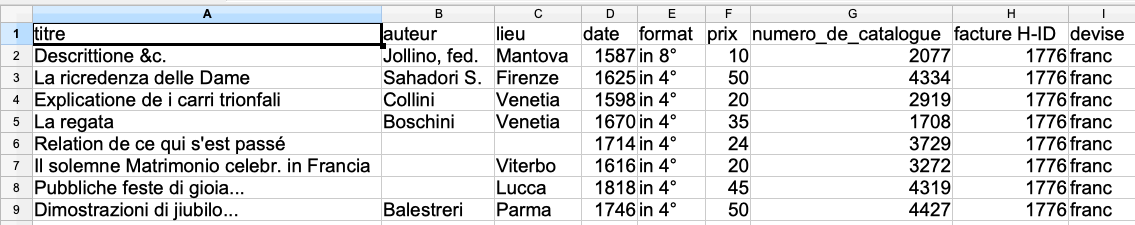
\includegraphics[width=15cm]{Images/CSV script python NuExtract3.png}
    \caption{Image du fichier CSV généré par le script.}
    \label{fig:csv-nuextract}
\end{figure}

\clearpage
\section{Exemple d'un dossier de factures numérisées}
\label{numerisation}
Le lien suivant permet de visualiser un dossier de factures Rondel numérisé et accessible sur Gallica : 
\url{https://gallica.bnf.fr/ark:/12148/btv1b108542870}

%\input{fichier.tex}

\newpage{\pagestyle{empty}\cleardoublepage}

%%%%%%%%%%%%%%%%%%

\backmatter % glossaire, index, table des figures, table des matières.. (la bibliographie a déjà été appelée)

\printindex % Appelle l'index des logiciels mentionnés dans le mémoire 
%\printglossaries[title=Glossaire]
%\listoftables


\listoffigures % Affiche la liste des figures 
\tableofcontents
\end{document}